%% 
%% ACS project dissertation template. 
%% 
%% Currently designed for printing two-sided, but if you prefer to 
%% print single-sided just remove ",twoside,openright" from the 
%% \documentclass[] line below. 
%%
%%
%%   SMH, May 2010. 


\documentclass[a4paper,12pt,oneside,openright]{report}


%%
%% EDIT THE BELOW TO CUSTOMIZE
%%

\def\authorname{Understanding and exploiting subspace organization in contextual word embeddings \xspace}
\def\authorcollege{David Yenicelik \\ ETH Zürich\xspace}
\def\authoremail{yedavid@ethz.ch}
\def\dissertationtitle{}
\def\wordcount{34'984}


%\usepackage[dvips]{epsfig,graphics} 
\usepackage{epsfig,graphicx,verbatim,parskip,tabularx,setspace,xspace}
\usepackage{amsmath, amsfonts}
\usepackage{bbm}
\usepackage{amsfonts}
\usepackage{amsmath}
\usepackage{siunitx}
\usepackage{caption}
\usepackage{subcaption}
\usepackage{empheq}
\usepackage{float}
\usepackage{url}
\usepackage{fancyvrb} % for "\Verb" macro
\usepackage{verbatim}
\usepackage{fancyhdr}
\usepackage[export]{adjustbox}
\usepackage{xcolor}
\usepackage{tcolorbox}

\usepackage[ruled,vlined]{algorithm2e}
\usepackage{tabularx,booktabs}

\newcounter{myverb}

\BeforeBeginEnvironment{verbatim}{%
\refstepcounter{myverb}%
\noindent\textbf{Example \themyverb}%
}

%TODO caption below table?

%TODO Implement glossary
% BERT
% nominalised verbs

%% START OF DOCUMENT
\begin{document}


%% FRONTMATTER (TITLE PAGE, DECLARATION, ABSTRACT, ETC) 
% \pagestyle{empty}
\pagestyle{fancy}

\fancyhf{}
\fancyhead[L]{\rightmark}
\fancyhead[R]{\thepage}
\renewcommand{\headrulewidth}{0pt}

\singlespacing
% title page information
\begin{titlepage} 

\begin{center}
\noindent
\huge
\dissertationtitle \\
\vspace*{\stretch{1}}
\end{center}

\begin{center}
\noindent
\huge
\authorname \\
\Large
\authorcollege      \\[24pt]

\includegraphics{CUni3.eps}
\end{center}

\vspace{24pt} 

\begin{center}
\noindent
\large
{\it A dissertation submitted to the University of Cambridge \\ 
in partial fulfilment of the requirements for the degree of \\ 
Master of Philosophy in Advanced Computer Science} 
\vspace*{\stretch{1}}
\end{center}

\begin{center}
\noindent
University of Cambridge \\
Computer Laboratory     \\
William Gates Building  \\
15 JJ Thomson Avenue    \\
Cambridge CB3 0FD       \\
{\sc United Kingdom}    \\
\end{center}

\begin{center}
\noindent
Email: \authoremail \\
\end{center}

\begin{center}
\noindent
\today
\end{center}

\end{titlepage} 

\newpage
\vspace*{\fill}

\onehalfspacing
\newpage
{\Huge \bf Declaration}

\vspace{24pt} 

I David Yenicelik of ETH Zürich, being a candidate for the M.Sc. ETH in
Computer Science, hereby declare that this report and the
work described in it are my own work, unaided except as may be
specified below, and that the report does not contain material that
has already been used to any substantial extent for a comparable
purpose.

\vspace{24pt}
Total word count: \wordcount

\vspace{60pt}
\textbf{Signed}: 

\vfill

This dissertation is copyright \copyright 2020 David Yenicelik. 
\\
All trademarks used in this dissertation are hereby acknowledged.



\newpage
\vspace*{\fill}

\singlespacing
\newpage
{\Huge \bf Abstract}
\vspace{24pt} 

One of the goals of Natural Language Understanding \textit{NLU} is to formalize written text in a way, such that linguistic features can be captured through computational models, which can then again be used for downstream machine learning tasks.
The most popular methodology in NLU is the use of vectors that represent written text, including word-vectors, sentence-vectors, etc. 
These vectors are often referred to as \textit{embedding} vectors, as they embed more complex concepts into a vector representation.

Because embeddings - due to their strong usage in downstream tasks - can be considered as the fundamental unit of machine learning in the domain of natural language, any shortcomings will influence the performance of the target task.
Given that language models such as BERT only capture a black-box function $f$ between input and output, our aim is to understand how the subspace organization relates to linguistic features.
We focus our analysis on \textit{semantics}, which captures a meaning within language, as this is one of the most important features of language. 
We analyse the BERT language model, as it provides a good balance between popularity, close to state-of-the-art performance, and generalizability to other modern language models.
\\

Our main contributions are the following: (1) We test for linear separability and ability to partition the space into semantic clusters within the sampled BERT vectors.
We show that while linear separability is possible, it is nearly impossible to find modes in the data which correspond to semantic classes that are as cleanly as defined by WordNet.
We conclude that BERT organized the embedding vectors imminently by context, and very little by semantics alone.
This can easily introduce undesirable properties such as strong sentiment, leading to considerable bias in downstream tasks.
(2) We analyze the relationship between part-of-speech and semantics. 
We show that these show a strong correlation in languages and that modern language models capture this strong correlation.
This affects the conclusion of some related work which had analysed language models which capture semantics, but which did not account for the correlation between part-of-speech and semantics.
(3) Finally, we introduce additional parameters for words whose sampled embedding vectors have high variance over the embedding space.
We investigate what downstream tasks are most affected  and use this as a proxy to understand what information is captured the most by the directions with high variance. \\

\newpage
\vspace*{\fill}


\pagenumbering{roman}
\setcounter{page}{0}
\pagestyle{plain}
\tableofcontents
\listoffigures
\listoftables

\onehalfspacing

% Definition of macros
\newcommand{\norm}[1]{\left\lVert#1\right\rVert}
%\newcommand{\bracket}[1]{\left[#1\right]}
\newcommand{\bracket}[1]{\left|#1\right|}
\newcommand{\absdet}[1]{\left|#1\right|}
\newcommand{\bftab}{\fontseries{b}\selectfont}
%% START OF MAIN TEXT 

\newcolumntype{b}{X}
\newcolumntype{s}{>{\hsize=.5\hsize}X}

\pagenumbering{arabic} 

\chapter{Introduction}
\setcounter{page}{1} 

One of the goals of Natural Language Understanding (\textit{NLU}) is to develop algorithms that are able to operate with human language.
However, it is not yet apparent that machines can think, or even operate with semantic concepts.
In most of these cases, the underlying language model uses heuristics, or black-box functions which simply maps an input text to output text merely satisfying the constraints set up by the target task.

 
These shortcomings can be addrressed by modelling written text in such a way that linguistic features can be captured.
Models can then be used for other machine learning tasks, referred to as \textit{downstream tasks}.
The most popular methodology in NLU is the use of vectors that represent written text, including word-vectors, sentence-vectors, and more. 
These vectors are often referred to as \textit{embedding} vectors, as they embed more complex concepts into a vector representation.
Optimally, the algebra of the space that we operate in, including the various operations such as multiplication and addition should have a meaningful correspondence to the concepts captured by these embeddings.
\\

Language representation models, also called Language Models (\textit{LM}) are a category of NLU models that can be used to generate word embeddings, sentence embeddings, and also intermediate representations that can be used for downstream tasks.
Most commonly, language models create vector representations by taking into consideration the context in which a word token occurs. 
Because embeddings - due to their strong usage in downstream tasks - can be considered as a fundamental unit in NLU, any shortcomings will influence the performance of the target task.
Improving the way these embeddings capture linguistic features has strong implications for a wide category of tasks including Named Entity Recognition (\textit{NER}), sentiment understanding, and automatic language-translation. 
However, most of the modern LMs are so complex that they are considered black-box models.
\\

We believe that providing a better understanding of the underlying principles will pave the way for future research to better track these issues.
The semantic attribute of a word is amongst the most important linguistic features.
It tells us what we mean when we say \texttt{dog} or \texttt{car}.
It can also be ambigious, when we use words such as \texttt{bank}, requiring us to look at the context to understand what meaning of \texttt{bank} one refers to.
Due to the significance of meaning in language, we will focus our analysis on how modern LMs capture semantics. 
Notice that the relation between language and thought is a much more fundamental and philosophical one.
Here, we assume that language is just an expression of thought, but that the two concepts are not equivalent.

\paragraph{Our main contributions are the following:}

\begin{enumerate}
\item We test to what extent the semantic subspace has multiple modes which correspond to meaning in language.
We test this by analysing linear separability between semantic classes, and test for clusterability in these structures.
We show that although linear separability is possible, it is nearly impossible to find modes in the data which correspond to semantic classes.
\item We analyze the relationship between the two linguistic features of part-of-speech and semantics. 
We show that these show a strong correlation in languages and that this correlation is reflected in modern language models.
This observation affects the conclusion made in some related work that analysed language models for semantics, but that did not account for the correlation between part-of-speech and semantics.
\item Finally, we introduce additional parameters for words whose sampled embedding vectors have high variance over the embedding space.
We investigate what downstream tasks are most affected  and use this as a proxy to understand what information is captured the most by the directions with high variance.
\end{enumerate} 

In this work we focus on BERT, as it provides a good balance between popularity, close to state-of-the-art performance, and generalizability to other modern language models.

Our findings show that although BERT does not capture a simple semantic subspace, but organizes the embedding vectory more broadly by context.
This can often introduce undesirable features such as strong sentiment, position in sentence, and thus lead to considerable bias in downstream applications.
We also show that sentiment is particularly more strongly captured in modern language models, allowing for language stereotypes to easily manifest itself, leading to stronger cases of bias in language models.

We will first start with summarizing the required background work (Section \ref{section:Background}), show existing analysis on the inner workings of BERT (Section \ref{section:RelatedWork}), conduct tests that do not modify the BERT model (Section \ref{section:UnderstandingBERT}) and make modifications to the embeddings in BERT to understand what effect this has on downstream tasks (Section \ref{section:ExploitingBERT}).
We will finally draw conclusion and show potential for future work (Section \ref{section:Conclusion}).


%\chapter{Background} 
\chapter{Background}\label{section:Background} 

\cite{harris54} was one of the early works that argue that there is an inherent structure in language and that this structure can be formalized.
They also mention that the relation between the linguistic representation in terms of sounds and tokens is related to the meaning that the representation entails. 
This representation is often captured in the form of a word token $w$, such as \Verb#bank# or \Verb#cat#.
The \textit{distribution hypothesis} of language was introduced in \cite{harris54}, and describes the idea that semantics and other linguistic features for a word $w$ can be purely extracted through the context that word $w$ occurs in.
However, despite the obvious relationship, the distinction between the distributional structure of the language and semantics is not a formal one. 
For the above case, the token \Verb#bank# may have different meanings $m_\text{bank-financial instution}$, $m_\text{bank-sea bank}$, whereas the token \Verb#cat# will have a more straight-forward semantic interpretation of $m_\text{cat-animal}$.
\cite{harris54} argues that there is a parallel semantic structure, and argues that this is not a one-to-one relation between vocabulary and different semantic classes.
Generally, one of the main views of this paper is that the meaning of a word is defined by the context it carries.
The formalization of language is not a trivial problem to consider, as this also touches base on a philosophical level \cite{hegel17}, \cite{wittgenstein53}, posing the question on the nature of the relation between thought and (language)-representation.

\section{Linguistic Features}

There is a vast number of linguistic features, going from phonological features, morphological and syntactic features to semantic features.
We will first introduce some linguistic features relevant to this work.
These make a formal analysis of our topic easier.

\paragraph{Polysemy} describes the phenomenon that a word token $w$ may have multiple meanings.
As a simple example, the number of meanings that \Verb#cat# can entail is $ | M_\text{cat} | = | \{ m_\text{cat-animal} \} |  = 1$, whereas the number of meanings that \Verb#bank# can entail is $ | M_\text{bank} | = | \{ m_\text{bank-financial instution},  m_\text{bank-sea bank}\} |  = 2$ (In fact, there are many more meanings of \texttt{bank}, but we will keep the examples concise).
The true numbers vary on the granularity chosen and the language at hand. 
The chosen granularity is a non-trivial question as this decides at what point one concept stops and another concept starts.
These definitions are often left to linguists to decide. \\

\paragraph{Part of Speech \textit{PoS}} implies the category of the syntactic function of a word.
Classes including adjectives \textit{ADJ}, adposition \textit{ADP}, adverbs \textit{ADV}, auxiliary \textit{AUX}, conjunction \textit{CONJ}, coordinating conjunction \textit{CCONJ}, determiner \textit{DET}, interjection noun \textit{INTJ}, noun \textit{NOU}, numeral \textit{NUM}, particle \textit{PART}, pronoun \textit{PRON}, proper noun \textit{PROPN}, punctuation \textit{PUNCT}, subordinating conjunction \textit{SCONJ}, symbol \textit{SYM}, verb \textit{VERB}, as is defined by \cite{spacyb}.
In this work, we will be using the spaCy python package  \cite{spacy} whenever we need to predict the part-of-speech class of a word-tokens and limit ourselves to high-level part-of-speech which consist of nouns, verbs, and adjectives.
For a more extensive list of linguistic features, please refer to section \ref{appendix:linguistic_features} in the Appendix.


\subsection{Tokens and n-grams}

A token is often considered the most basic unit of language.
In the above sections, we have implicitly assumed that this token is always a word $w$ . 
However, there is a variety of ways that sentences can be encoded into a sequence of tokens.
We will go over some forms that tokens can take on, starting with the most trivial ones.
In a sentence such as

\begin{tcolorbox}
\begin{verbatim}
The man travelled down the road.
\end{verbatim}
\label{sentence:man_travelled}
\end{tcolorbox}

the set of word-tokens would constitute of $\{ \text{down}, \text{man}, \text{road}, \text{the}, \text{traveled} \}$.
The way a sentence is split up into an ordered array of individual tokens is referred to as \textit{tokenization}.
Tokenizing the above sentence (assuming we only allow lower-case tokens) would result in 

$$
[the, man, traveled, down, the, road]
$$

It is important to note that there are also other ways to interpret language tokens. \\

\textbf{Characters} can be considered as another set of tokens language.
Looking at example \ref{sentence:man_travelled}, the set of basic units would correspond to the Latin alphabet plus whitespace and numbers $a - z" "0-9$ (" " denotes whitespace), and the above sentence would be tokenized into the sequence 

$$
[t, h, e, " ", m, a, n, " ", t, r, a, v, e, l, e, d, " ", d, o, w, n, " ", t, h, e, " ", r, o, a, d]
$$

Choosing characters as the basic token levels has shown considerable success and popularity in language modeling \cite{sutskever11} and translation \cite{lee17}.

\paragraph{Byte pair encodings} \cite{gage94} presents another popular mechanism to tokenize sentences, and also shows success in the case of language modeling and translation \cite{sennrich16}. 
Here, the most frequent pair of bytes in a sequence is replaced with the most frequent pair of bytes in a sequence with a single, unused byte, similar to Huffman encoding.
This can also be used as a compression scheme.

Depending on what corpus this tokenizer is trained on, the above sentence could be tokenized into the following sequence

$$
[the., " ", ma., n., " ", t., rav., e., led., " ", do., w., n., " ", the., " ", r., oa., d.]
$$

The tokenization of the sentence above implies that the corpus that the tokenizer was trained on includes as a majority of word-occurrences the sequence of characters \texttt{the}, as well as \texttt{lled} and \texttt{do}. 
The dot at the end of each character denotes the end of a byte-pair token.
The main idea behind this tokenization is to construct a vocabulary of frequent subwords, allowing to generalize to unseen words.

\paragraph{WordPiece tokenizer} \label{tokenizer:WordPiece} \cite{wu16} follows a similar idea as the byte-pair encoding and constructs a vocabulary given a corpus by maximizing entropy.
The main difference to the byte-pair encoding is that the vocabulary naturally includes a set of the most commonly appearing words in the respective language, and is then aggregated by introducing additional subword units to cover unseen character sequences.

%TODO man travelled never works ...
The tokenization of Example \ref{sentence:man_travelled} would then look as follows (depending on which implementation and version of the WordPiece tokenizer is used)

$$
[the, man, travel, \#\#led, down., the, ro,  \#\#ad.]
$$

where we can see that words such as \Verb#the# and \Verb#down# are not further divided into tokens and that suffixes such as \Verb!##led! are introduced, because these are unregular patterns which allow for better generalization.






\section{Word Embeddings}

We will now present ways to capture relations between tokens by representing these through vectors. \\

\textbf{Word-Embeddings:} In general, we want to find a mapping 

\begin{equation}
\label{map:embedding_mapping}
w \mapsto (x_w, b_w) \in \mathcal{X}^{d + 1}
\end{equation}

where $w$ is a token representation from a vocabulary $w \in V$ and where this token representation is transformed into a $d+1$-dimensional vector representation $x_w$, and a bias-term $b_w$ that is specific to the token $w$.
Whenever we talk about \textit{word-vectors}, \textit{(word)-embeddings}, or \textit{feature-vectors}, we will refer to the image of the above map (Equation \ref{map:embedding_mapping}). 
For convenience and unless stated otherwise, we will assume that $x_w$ absorbs the bias term $b_w$ as an additional vector-element.
Also, for simplicity and unless otherwise stated, we will use the euclidean real-valued vector-space $\mathbb{R}^{d+1}$ to described the resulting embedding vectors.
Please note, however, that the choice of the embedding space $\mathcal{X}$ is not fixed in general, and as such, work in other spaces such as hyperbolic spaces  \cite{ganea18} have also been conducted. \\

\textbf{Distance:} Our goal is to build an embedding space where the distance between word-embeddings correspond to the relation between words (i.e. the semantics entailed by their tokens).
We introduce the concept of \textit{distance} $d : \mathcal{X}  \times \mathcal{X} \mapsto [ 0, \inf )$, which captures a relation between two elements. 
For a set of elements $x, y, z \in \mathcal{X}$, following properties must hold for a mapping to be a valid distance metric:

\begin{enumerate}
\item $d(x, y) \geq 0$ (non-negativity)
\item $d(x, y) = 0 \iff x = y$ (identity)
\item $d(x, y) \leq d(x, z) + d(z, y)$ (triangle inequality)
\end{enumerate}{\label{def:distance}}

One consequence of the above properties is that for words $a, b, c$, each having a word embedding $x, y, z$ respectively, $d(x, y) < d(x, z) \iff $ word instance $b$ is conceptually closer to word $a$ than word $c$.
For convenience, whenever we input $a, b, c$ into the distance function $d(\cdot, \cdot)$, the word-embeddings for the corresponding word-tokens shall be used to numerically calculate the distance.
Also, please notice that we did not include the notion of symmetry for distance measures. \\

\textbf{Learning a distance:}
A popular paradigm in machine learning is to maximize a posterior probability distribution given some data $\mathbf{X}$.
One can now follow the idea of the \textit{distributional structure} of language \cite{harris54}, which states that all linguistic features for a word $w$ can be captured by lookin at its context words.
In terms of word vectors, we want to maximize the probability that $w$ occurs in the context window of $w \prime$ through some parameters $\theta$.
Implicitly, this corresponds to minimizing the distance between $x_w$ and $x_w^{\prime}$, while keeping the distance between $x_w$ and all other word-vectors constant. 
We call $w \prime$ a \textit{context word} for $w$, and consequently we want to maximize the probability for any two co-occurring words $w, w^{\prime}$:

\begin{equation}
p \left(w | w^{\prime}\right) \nonumber
\end{equation}

In many cases, maximizing the likelihood probability corresponds to minimizing the global distance between co-occurring words.

\begin{equation}
\forall w, w^{\prime} : \hspace{20pt} \text{max } p \left(w | w^{\prime}\right) \iff \text{min } d(w | w^{\prime})
\end{equation}

Please note that we do not state that the minimization problem is the dual of the maximization problem. \\

\textbf{Exploiting the distributional structure of language:} Our goal is to learn distances between words by exploiting the distributional structure of a set of sentences.
A set of sentences which we use for this task is called a \textit{corpus}. 
One of the early formalizations of representing the distributional structure of words is explained in \cite{bengio03}, which argues that a sequential statistical model can be constructed to estimate the true posterior of a sequence of tokens.  
In it's most naive form, this would imply that we can estimate the probability of a sequence of words $\mathbf{w}$ as

\begin{equation}
p(\mathbf{w}) = \prod_{t=1}^T p\left( w^{(t)} | w^{(t -1)}, \ldots, w^{(1)} \right)
\label{eq:naive_sequential_probability}
\end{equation}

where $\mathbf{w} = w^{(1)}, \dots, w^{(T)} $ is the sequence of words and $p(\mathbf{w})$ the probability of this sentence occurring.
This corresponds to an autoregressive model.
One could for example use (hidden) markov models to model this relation, as we could fix the \textit{context size} $n$ (in this case, only looking at previously occurring words) and exploit the $n$-step markovian assumption of

\begin{equation}
p\left( w^{(t)} | w^{(t -1)}, \ldots, w^{(1)} \right) = p\left( w^{(t)} | w^{(t -1)}, \ldots, w^{(t - n + 1)} \right)
\end{equation}\label{eq:naive_sequential_probability_markovian}

Fixing the context window to $n$ words for each computation (i.e. convolution), introduces the concept of \textit{n-grams}. 
An n-gram is a sequence that consists of $n$ tokens.
n-grams can also occur with characters, where $n$ characters are fed in to some model at a certain timestep $t$.

Next to a context which only consists of the \textit{previous} $n$ words, one can also regard a context which includes both the previous \textit{and subsequent} $R$ words. 
Combining this with a probability model which assumes conditional independence between all but one context word, this leads us to

\begin{equation}
p(\mathbf{w})=\prod_{t=1}^{T} \prod_{\triangle \in \mathcal{I} } p\left( w^{(t)} | w^{(t +\Delta)}\right)
\label{eq:naive_coocurrence_probability}
\end{equation}

whose probability we wish to estimate (and maximize if this is in the given training dataset) with $\mathcal{I}=\{-R, \ldots,-1,1, \ldots, R\}$ as the extent of the context window. \\

\textbf{Loss Objective:} Given that computational power is limited, we are usually interested in learning a parametrized model which captures this underlying distribution behind equation \eqref{eq:naive_coocurrence_probability}.
One way to learn this parametrized model is to \textbf{maximize} a loss by backpropagating the gradients of the parameters.
In that case, the loss function would look as follows.


\begin{equation}
\mathcal{L}(\theta ; \mathbf{w})= \prod_{t=1}^{T} \prod_{\triangle \in \mathcal{I}} p_{\theta}\left(w^{(t)} | w^{(t +\Delta)}\right)
\end{equation}{\label{eq:basic_equation_log_maximization}}

By maximizing the mean loss over all sentences in a big-enough corpus $\mathcal{C}$, we can find a reliable estimator model with parameters $\hat{\theta} = \text{argmax}_\theta \mathcal{L}(\theta ; \mathbf{w})$ using a maximum likelihood estimation approach.
One would usually rephrase this as a log-loss problem as this allows for the gradients to be more easily computed and avoids numerical issues.

Intuitively the above distributions implement the idea  behind \cite{harris54} very well, specifically the property that the meaning of a word is captured by the context that it occurs in.
The above equations follow a \textit{continuous bag of words CBOW} approach, which aims at predicting a target word $w^t$ given some context words $w^{\prime}$.
In contrast, it is also possible to follow a \textit{skip-gram SG} approach, where the aim is to predict context words $w^{\prime}$ given a target word $w^t$.
Training a model using the skip-gram approach does not change the search space of models $\theta \in \Theta$.
The final chosen model $\hat{\theta}$ will likely be different, however.
The skip-gram model is found to work better with rare words, whereas the CBOW model seems to have slightly better accuracy on words that are occurring more frequently.

\begin{figure}[h]
	\center
  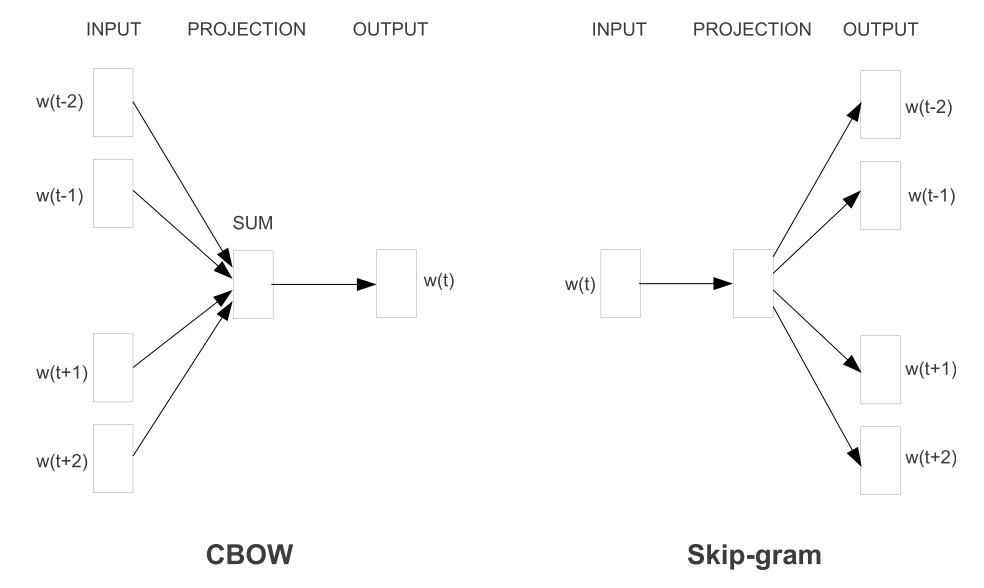
\includegraphics[width=0.6\linewidth]{./assets/background/cbow_and_skipgram.png}
  \caption{Figure taken from \cite{mikolov13}. The CBOW model (left) predicts the current word based on the context. The skip-gram model (right) predicts surrounding words given the current word.}
  \label{fig:cbow_skipgram}
\end{figure}

Using a skip-gram approach, the loss captured through equation \eqref{eq:basic_equation_log_maximization} would be reformulated into 
\begin{equation}
\mathcal{L}(\theta ; \mathbf{w})=\prod_{t=1}^{T} \prod_{\triangle \in \mathcal{I}} p_{\theta}\left(w^{(t +\Delta)} | w^{(t)}\right)
\end{equation}{\label{eq:basic_equation_log_maximization_skipgram}}

Although we have mentioned that the probability density distribution $p$ is often modelled through a parametrized function (due to the sheer amount of data within corpora), we have not presented methods on how this parametrization can be achieved.
In the following section, we will show how vectors for $x_w$ and $b_w$ can be found, and other ways to parametrize the probability density function $p$.
We will not go into too much detail as to how these models are trained, as all of them can be trained by applying a gradient-based optimization routine on the loss term and updating the weights accordingly.

\subsection{Static Word Embeddings}

Here we will talk about word-embeddings where each word-token only has a single embedding $x_w$, i.e. there is a bijection between word-tokens and word-embeddings. 
Specifically, the mapping in equation \eqref{map:embedding_mapping} is not a probabilistic function with a latent random factor.
We will start with simple static word embeddings and proceed to more complex models in subsequent sections.

\subsubsection{Basic Model}

The first model we are going to look at is a most basic model which fulfills the properties of the distance metrics shown in equation \eqref{def:distance} and minimizes words within the same context.

Here, we introduce a \textit{log-bilinear} \cite{cil_slides} model where the log-probability is defined as

\begin{equation}
\text{log} p_{\theta}(w | w^{\prime}) = \left\langle\mathbf{x}_{w}, \mathbf{x}_{w^{\prime}}\right\rangle+b_{w} + \text { const. }
\end{equation}

The actual probability density function can be calculated by exponentiating the log-probability

$$
p_{\theta}\left(w | w^{\prime}\right)=\frac{\exp \left[\left\langle\mathbf{x}_{w}, \mathbf{x}_{w^{\prime}}\right\rangle+b_{w}\right]}{Z_{\theta}\left(w^{\prime}\right)}
$$

where $Z_{\theta}\left(w^{\prime}\right):=\sum_{v \in \mathcal{V}} \exp \left[\left\langle\mathbf{x}_{v}, \mathbf{x}_{w^{\prime}}\right\rangle+b_{v}\right]$ is a normalization constant such that the probability mass sums to $1$.
The model parameters consist of the word-embeddings $  \theta = \{ (x_w, b_w ) \in \mathbb{R}^{d+1} | \forall w \in V \}$.
We can use a gradient-based loss-minimizing (notice the log-term) method which minimizes the cost function for $\theta$, for a word $w$ and all their possible context words $w^{\prime} = w^{(t+\Delta)}$ within a context window $R$.

$$
\mathcal{L}(\theta ; \mathbf{w})=\sum_{t=1}^{T} \sum_{\Delta \in \mathcal{I}} \log p_{\theta}\left(w^{(t+\Delta)} | w^{(t)}\right)
$$

This basic model comes with drawbacks. 
The distance would be minimized if all word-embeddings would collapse onto a single point. 
No term forces unrelated words to move away from each other, although this is a property that we are interested.
Such a term would result in more isotropic vector models, that has also shown practical performance \cite{ethayarajh19}.


\subsubsection{Word2Vec}

One of the most prominent word vector models is proposed in \cite{mikolov13, mikolov13b}.
Here, a neural network with a single embedding layer can be trained to transform one-hot-vectors $\in \{ 0, 1 \}^{| \mathcal{V} |}$ (representing words $w$ in avocabulary $\mathcal{V}$)
into an embedded representation $x_w \in \mathbf{R}^{d + 1}$.
As the neural network consists of a single layeer, this boils down to a linear embedding matrix $W$ acting as a lookup table.
Both a continuous bag of word and also a continuous skip-gram approach can be used.
The skip-gram approach is preferred in practice.
Specifically, the loss-function that is optimized looks as follows

\begin{align} 
\mathcal{L}(\theta ; \mathbf{w}) & =\sum_{t=1}^{T} \sum_{\Delta \in \mathcal{I}} [ \nonumber \\ 
& b_{w^{t+\Delta}} +\left\langle \mathbf{x}_{w^{(t+\Delta)}}, \mathbf{x}_{w^{(t)}} \right\rangle \nonumber  \\
& -\log \sum_{v \in \mathcal{V}} \exp \left[\left\langle\mathbf{x}_{v}, \mathbf{x}_{w^{(t)}}\right\rangle+b_{v} \right] 
\end{align}

As one can see, the loss function takes as input the bilinear loss from the basic model.
This is complemented by a regularizing term (last line), such that random samples are not all next to each other in the embedding space produced.
This idea is referred to as \textit{negative sampling}.

\begin{figure}[h]
	\center
  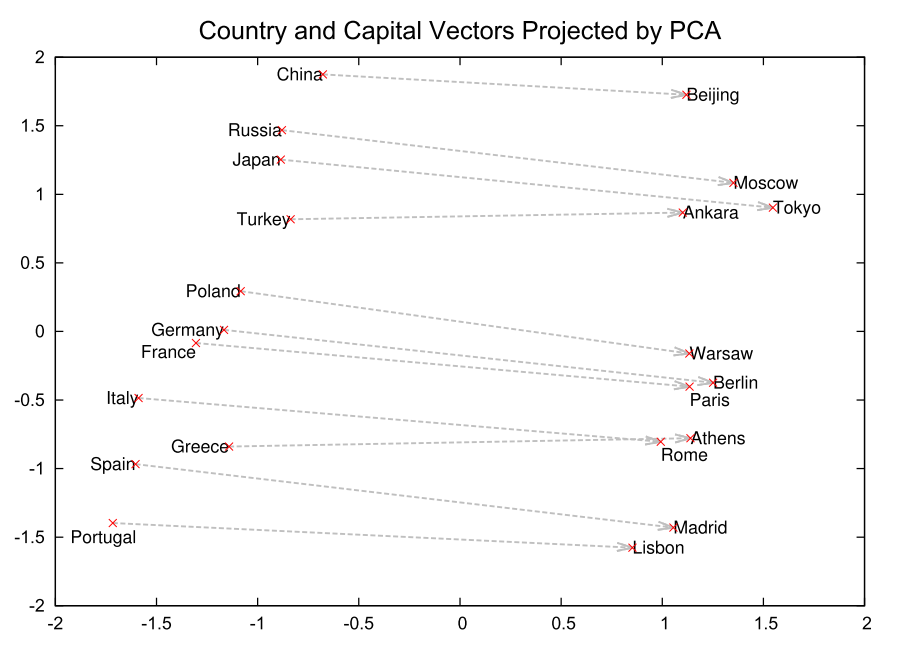
\includegraphics[width=0.6\linewidth]{./assets/background/word2vec_cities.png}
  \caption{Figure taken from \cite{mikolov13b}. A 2-dimensional PCA projection of the 1000-dimensional skip-gram vectors of countries and their capital cities. The proposed model is able to automatically organize concepts and learn implicit relationships between them. No supervised information was provided about what a capital city is.}
  \label{fig:cbow_skipgram}
\end{figure}

Backpropagation is used to optimize the networks weights. 
Also, highly frequent words are optionally subsampled and their frequency is re-weighted using the formula $$
P\left(w_{i}\right)=1-\sqrt{\frac{t}{n\left(w_{i}\right)}}
$$

where $n( \cdot )$ is the function that returns the frequency of a word $w_i$ in a given corpus.

\subsubsection{GloVe}

For the global vectors for word representation \textit{GloVe} \cite{pennington14}, the authors follow a matrix factorization approach.
First, a global co-occurrence matrix is created $\mathbf{N} = (n_{ij}) \in \mathbb{N}^{|\mathcal{V}| \dot |\mathcal{C}|}$ where each entry $n_{ij}$ is determined by the number of occurrences of word $w_i \in \mathcal{V}$ in context $w_j \in \mathcal{C}$.
Given that the vocabulary size can exceed multiple thousand items, this practically results in a sparse matrix.

\begin{align}
\mathcal{H}(\theta ; \mathbf{N}) &=
\sum_{i, j} f\left(n_{i j}\right)(\underbrace{\log n_{i j}}_{\text {target }}-\underbrace{\log \tilde{p}_{\theta}\left(w_{i} | w_{j}\right)}_{\text {model }})^{2} \\
&= \sum_{i, j} f\left(n_{i j}\right)(\log n_{i j} - \left\langle x_i, y_j \right\rangle )^{2} \\
\end{align}

where $f(n_{ij})$ is the weighting function which assigns a weight for each entry in the co-occurence matrix based on the co-occurence of words $w_i$ and $w_j$. 
In the second line, we also again use a bilinear model $\tilde{p}_{\theta}\left(w_{i} | w_{j}\right) \propto \exp \left[\left\langle\mathbf{x}_{i}, \mathbf{y}_{j}\right\rangle+b_{i}+c_{j}\right]$.
The constants $b_i, c_j$ are left out and are assumed to be absorbed in the embedding vectors.
A popular choice for the weighting function is 
$
f(n) = \min \left\lbrace 1, \left(\frac{n}{n_{\max}}\right)^{\alpha} \right\rbrace
$
with $\alpha \in (0, 1]$.
The motivation behind this is that frequent words should not be have too much weight for the loss-terem (there is a cutoff at some point, as the number of word-occurrences increase exponentially).
Word that have a too small count are considered noise and slowly cancelled out. \\


Similar work to word2vec and GloVe exists (i.e. fastText \cite{bojanowski17}).
Further extensions include word embeddings as probability densities using a Bayesian skip-gram approach \cite{brazinskas19}, where the resulting model architecture is similar to the word2vec neural network, but includes a probabilistic latent module.
Another line of work \cite{yan19} aims to exploit the formal properties of Wasserstein distances to learn static word embedding.
Please refer to section \ref{appendix:GaussianEmbeddings} in the appendix where we present Gaussian Embeddings \cite{vilnis14} for an explanation of what such a probabilistic extension could look like.

\subsection{Contextual Word Embeddings}

In contrast to static word embeddings, contextual word embeddings rely not only on the target word $w$ as input, but also require a subset of the context $[c_1, \ldots, c_{i-1}, c_{i+1}, \ldots, c_T]$ around $w$ as input.
Specifically, the mapping \eqref{map:embedding_mapping} is modified in such a way to take as input the previous context words $c_\text{previous} = w^{(t)}, \ldots, w^{(t-d + 1)}$, and optionally also the subsequent context words $c_\text{subsequent} = w^{(t-d - 1)}, \ldots, w^{(1)}$.

\begin{equation}
(c_\text{previous}, w, c_\text{subsequent}) \mapsto (x_w) \in \mathcal{X}^{d + 1}
\end{equation}{\label{map:context_embedding_mapping}}

As an example, while static word embeddings would produce the same vector $x_0$ for all occurrences of the word $bank$, the contextual word embedding would produce different embeddings $x_1$, $x_2$ and $x_3$ respectively for the three sentences:

\begin{tcolorbox}
\begin{verbatim}
I withdrew some cash at the bank's ATM.
The bank was closed.
I walked down the sea bank.
\end{verbatim}
\end{tcolorbox}

Any change in the context words will generally result in a different embedding $x$.
Capturing this logic through a probability density function, we now calculate the probability

\begin{align}
p(w^{(t-d)} | c_\text{previous}, w^{t-d}, c_\text{subsequent}) &= p(w^{(t-d)} | w^{(t)}, \ldots, w^{(t-d + 1)}, w^{(t-d)}, w^{(t-d - 1)}, \ldots, w^{(1)})
\end{align}{\label{eq:transformer_probability}}

There are different ways to capture this probability, from simple markov models, to LSTMs, to transformers.
We will go over the most prominent models of recent years. \\

\begin{figure}[h]
	\center
  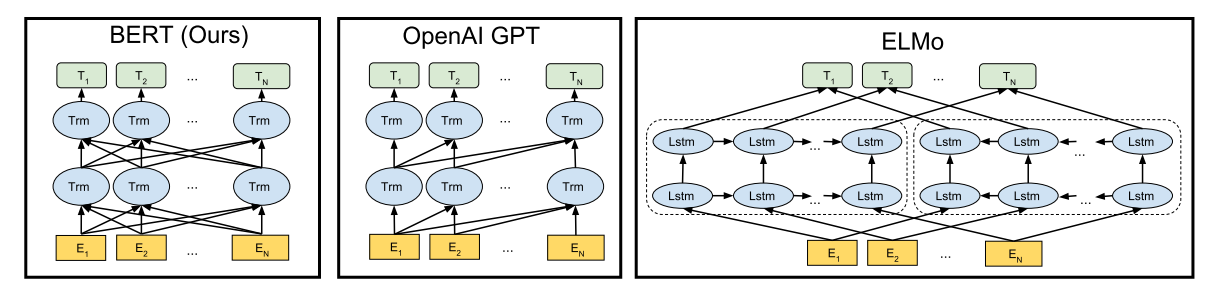
\includegraphics[width=\linewidth]{./assets/background/BERT_GPT_ELMo.png}
  \caption{Figure taken from \cite{devlin18}. BERT uses a bidirectional transformer, which reads in all the input for both the previous and subsequent context. OpenAI GPT (next section) uses a left-to-right Transformer, reading in only the previous context. ELMo uses a bidirectional LSTM which naturally captures a single direction per LSTM, thus both previous and subsequent context is read. }
  \label{fig:attention_is_all_you_need}
\end{figure}

\subsection{ELMo}

On of the simplest models to produce contextual word embeddings, is the \textit{Embeddings from Language Models} (ELMo) model proposed by \cite{peters17b}.

%which take into account more than just a single word, but all tokens from the context $\mathbf{c} = (c_\text{previous}, c_\text{subsequent}) $
ELMo contains the Long Short-Term Memory \textit{LSTM} memory cell as it's basic unit.
To get a short overview of the architecture of the LSTM cell, and the resulting recurrent neural network, we refer the reader to Section \ref{appendix:LSTM} in the Appendix.
When we make use of two LSTM networks, one that reads the sequence in the positive direction (i.e. $[\ldots, x_{t-1}, x_t, x_{t+1}, \ldots]$ in this particular direction) and another one that reads the sequence in a negative direction (i.e. $[\ldots, x_{t+1}, x_t, x_{t-1}, \ldots]$), the resulting architecture is called a \textit{bidirectional LSTM}, also called \textit{biLSTM}.
ELMo consists of two layers of such bidirectional LSTMs, where the output of the first layer is fed in as the input to the second layer.
Specifically, the loss function that the language model optimizes during unsupervised training results in 

\begin{align} 
\sum_{k=1}^{T} &\left(\log p\left(w_{k} | w_{k-1}, \ldots, w_{1} ; \Theta_{x}, \vec{\Theta}_{L S T M}, \Theta_{s}\right)\right.\\
+&\left.\log p\left(w_{k} | w_{k+1}, \ldots, w_{T}; \Theta_{x}, \overleftarrow{\Theta}_{L S T M}, \Theta_{s}\right)\right) 
\end{align}

where $p$ is the output of an LSTM model parametrized by it's weights $\theta$, including a softmax head to arrive at a valid probability distribution amongst candidate words in the vocabulary $\mathcal{V}$.

Given that the LSTM is a sequential model, it outputs as many hidden representations as there are timesteps $T$ that are given as input to the model. 
The forward LSTM reads in the previous context $c_\text{previous}$ whereas the backward LSTM reads in the subsequent context $c_\text{subsequent})$.
Each LSTM layer produces one set of such hidden representations.
ELMo concatenates the hidden representations for both of the bidirectional LSTM layers to arrive at a single contextual word embedding $x_{w_i} = [h^\text{backward}_{w_i}, h^\text{forward}_{w_i}]$.

Formally, one would pre-train this model on a huge corpus in a supervised way through masked pre-training where the input sequence $[w_1, \ldots , w_i, \ldots, w_T]$ is also expected as the output sequence offset by one timestep $[w_2, \ldots, w_{i+1}, \ldots , [PAD] ]$.
For further details on pre-training ELMo we refer the reader to \cite{jozefowicz16}.
This pre-trained language model would then be extended by another linear layer or RNN, which would be adapted for a downstream task.
This downstream task could be named entity recognition, part of speech tagging etc.
The gradients of the ELMo biLSTM model are frozen and updated during fine-tuning.
Thus, only the weights of the task-specific parameters are optimized. 

\subsection{The Transformer Architecture}

Although ELMo creates contextual word embeddings, the performance is limited to LSTMs.
Specifically, the LSTM used within ELMo is a sequential timestep model which covers a storage mechanism within the weights it uses, theoretically resulting in a 1-step markov model

\begin{align}
p(w_1, \ldots, w_T) &= p(w_T | w_{T-1}; h_{T-1}, \theta) \nonumber  \\
& \ldots p(w_t | w_{t-1}; h_{t-1}, \theta) p(w_{t-1} | w_{t-2}; h_{t-2}, \theta) \nonumber \\
& \ldots p(w_1 ; \mathbf{0}, \theta) 
\end{align}

where $h_{i}$ is the forward-propagation vector outputted by the LSTM cell at timestep $i$, which are supposed to "store" inforrmation.
Although intuitively $h_{T-1}$ is supposed to capture information from many timesteps back, there is no explicit information flow between the LSTM cell at timestep $t+1$ and $t-1$ (i.e. any two cells which are more than 2 steps away).

The transformer architecture \cite{vaswani17} (depicted in Figure \ref{fig:attention_is_all_you_need}) addresses this shortcoming.
It introduces the concept of attention for use by modern language models, which can model relations between any two input tokens $w_i, w_j$ with $i \neq j$ and $| i - j |  > 1$.
For a more detail treatment of the attention mechanism, we refer the reader to \cite{bahdanau16}.
% A single transformer takes as input a sequence $\mathbf{w} = [w_1, \ldots, w_T]$ and outputs a set of hidden.
The attention mechanism takes all the intermediate token representations for the full sample sentence (not exclusively for the previous or subsequent context) and calculates a correlation score between the hidden representations of each timestep.
The transformer outputs an intermediate representation which can be converted to softmax probabilities through a linear head.

\begin{figure}[H]
	\center
  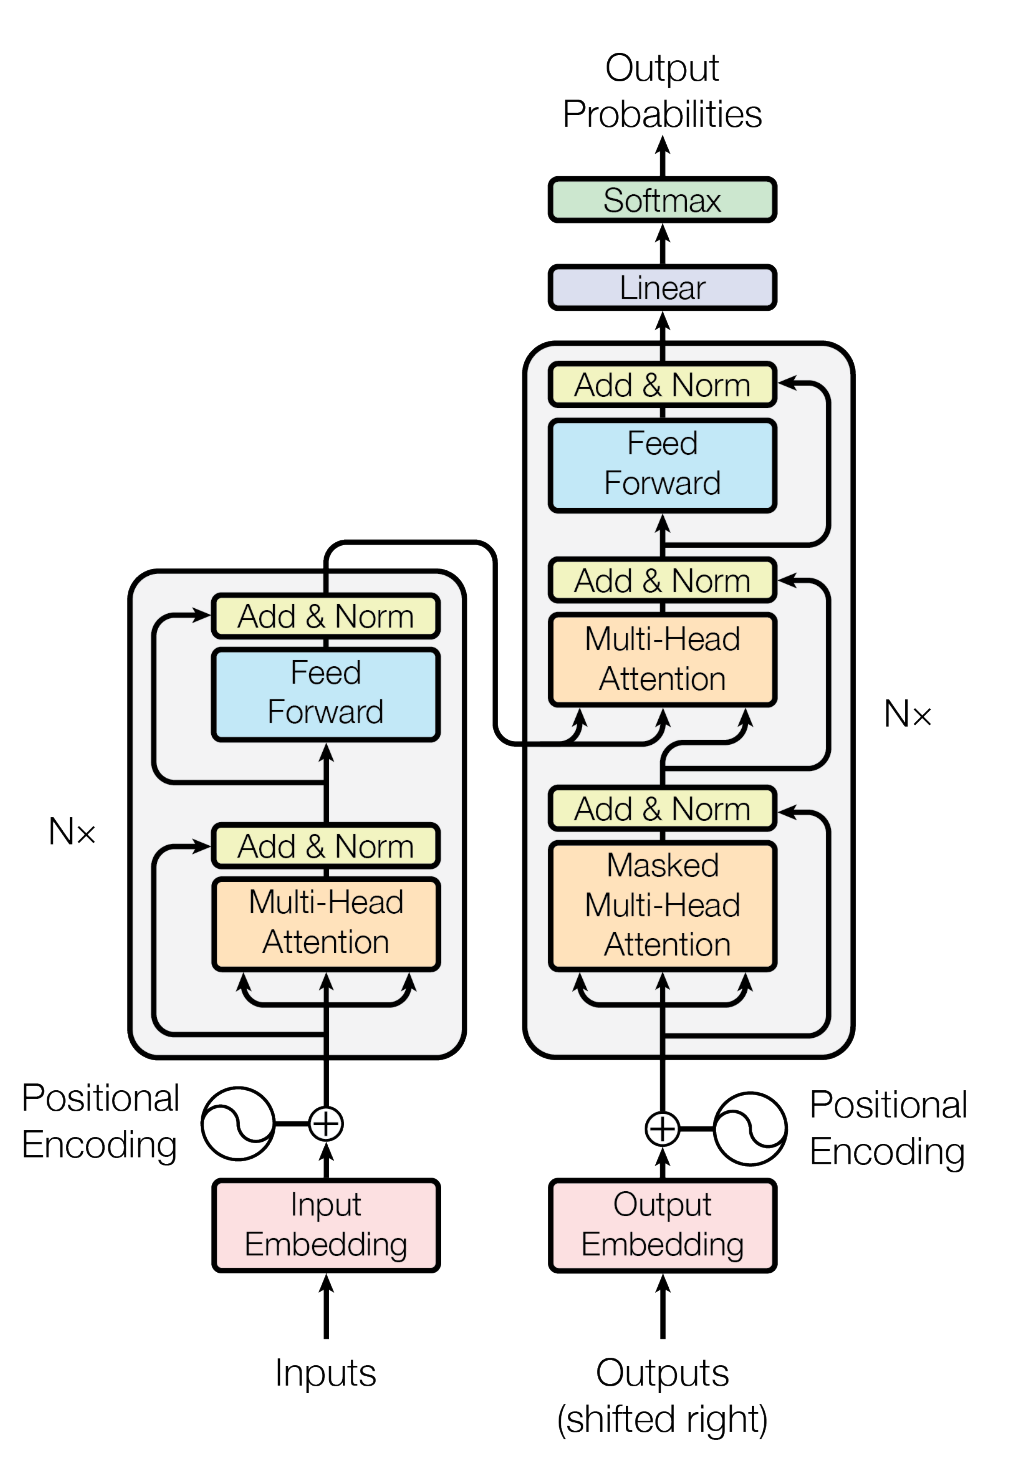
\includegraphics[width=0.5\linewidth]{./assets/background/transformer_module.png}
  \caption{Figure taken from \cite{vaswani17}. The architecture of the transformer module which encapsulates multiple attention modules.}
  \label{fig:attention_is_all_you_need}
\end{figure}

This allows for the model to explicitly capture and exploit a similarity metrics between any two input elements of the sequence.
This has implications for the complexity of the model.
Instead of calculating the raw probability of \eqref{eq:naive_sequential_probability}, and even using a markovian assumption because computation power is expensive, the transformer architecture implicitly calculates the joint probability of an entire sequence of words.
This decreases the number of computation-steps through which information flows. \\

\subsection{BERT: Bidirectional Encoder Representations from Transformers}\label{section:BERT}
 
The Bidirectional Encoder Representations from Transformers \textbf{BERT} \cite{devlin18} is a language representation model that makes use of the transformer architecture in contrast to ELMo, which uses recurrent neural networks as its underlying modules.
Although there are different version of BERT published, the base model of BERT consists of 12 attention layers, which output a 768-dimensional hidden representation of the input sequence.
This hidden representation - which is produced for each item in the input sequence - can be used for downstream tasks as is interpreted as the contextual word embedding for each token $w_i$ of the input-sequence $s$.

The main advantage of BERT is the more direct information flow through the attention mechanism. 
Formally, the attention mechanism allows for a direct comparison of hidden states $h_t$ and $h_k$ with ($|t - k| > 1$).
These hidden states $h_t$ and $h_k$ can be interpreted as context  embeddings for the word $w_t$ and $w_k$ which are passed as the sequence $[w_1, \ldots, w_t, \ldots, w_k, \ldots, w_T]$ into BERT.
In contrast  an LSTM would contain a single hidden state $h_{t-1}$ passed forward at every timestep, which would have to contain the information for all previous words $h_k$ where $k < t - 1$.
Stacking the transformer for multiple layers allows BERT to capture a complex structure of language.

BERT is \textbf{pre-trained in two phases}. 
In the first phase BERT is trained using a \textbf{masked language model} approach. 
Sentences with a maximum length are sampled from a corpus.
About 15\% of words in the sentence are replaced with the \texttt{[MASK]} token, and the weights are optimized in such a way to predict the word which was replaced by the \Verb#[MASK]# token.

\begin{tcolorbox}
\begin{figure}[H]
\begin{verbatim}
[CLS] The man went to [MASK] store. [SEP]
\end{verbatim}
Example from \cite{devlin18}. 
An sentence where 15\% of the tokens are replaced with the [MASK] token. 
During the first phase of pre-training, the weights of the BERT model are optimized in such a way to predict the true underlying words.
The word to be predicted is \texttt{the}.
\end{figure}
\end{tcolorbox}

The second pre-training phase is a \textbf{Next Sentence Prediction} task, where BERT is supposed to predict a sentence $s_i$ given its predecessor sentence $s_{i-1}$ in a fulltext corpus.
This is a binarized task, which means that given inputs $s_{i-1}$, $s_r$, BERT is supposed to predict whether or not sentence $r = i$ (i.e. whether $s_r$ is the subsequent sentence to $s_{i-1}$, or whether $s_r$ is some randomly sampled sentence).
50 \% of the training set here consists of randomly sampled sentences, and the other 50 \% of the training set consists of the actual next sentence for a given corpus.

\begin{tcolorbox}
\begin{figure}[H]
\begin{verbatim}
[CLS] the man went to [MASK] store [SEP]
he bought a gallon [MASK] milk [SEP]
\end{verbatim}
Example from \cite{devlin18}. 
Two input sequences which where 15\% of the tokens are replaced with the [MASK] token. 
During pre-training, the weights of the BERT model are optimized in such a way to predict the true underlying words.
In this case, the second sentence is a continuation of the first one, and thus the label would be \texttt{isNext}.
\end{figure}
\end{tcolorbox}

Pre-training which is applied on a 3.3 billion word corpus.
For fine-tuning to specific downstream tasks, the learning rate is put lower than during pre-training.
The gradient updates all model weights.
One can apply an additional linear layer on top of the $T$ hidden representations produced, use RNNs or more complex models, or use specialized outputs in BERT for downstream prediction tasks.

\begin{figure}[h]
	\center
  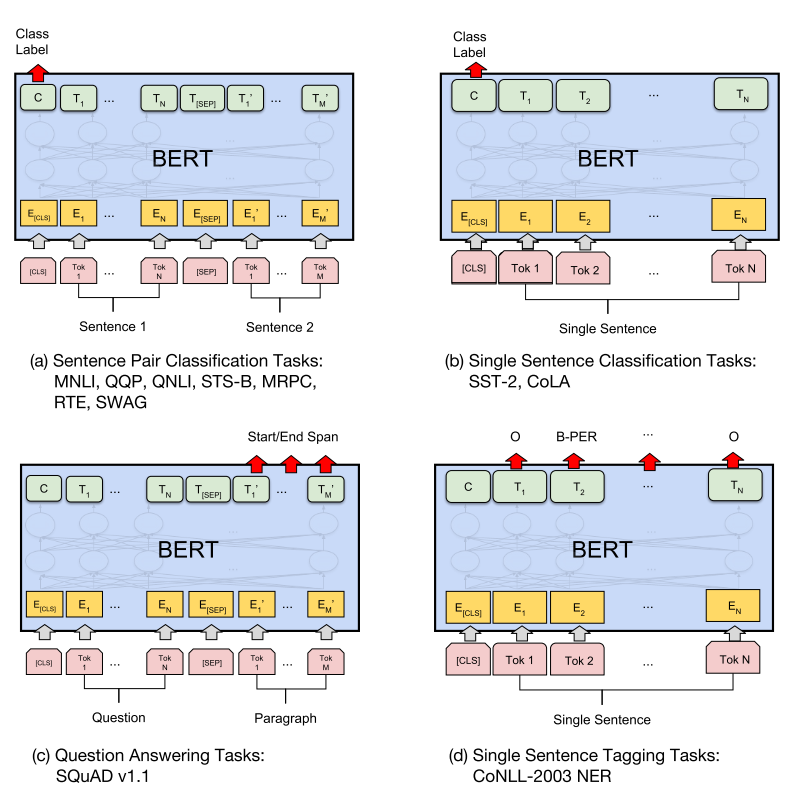
\includegraphics[width=0.8\linewidth]{./assets/background/BERT_GLUE_finetune.png}
  \caption{Figure taken from \cite{devlin18}. Ways to fine-tune BERT on different GLUE tasks.}
  \label{fig:cbow_skipgram}
\end{figure}

Multiple versions of BERT are provided, including $BERT_{LARGE}$ and $BERT_{BASE}$, each taking as input a sequence of maximal length 512, as the learned attention weights inside the transformer architecture only allow a maximal sequence length. 
Because we will make modifications to the inner workings of BERT, and mostly to the transformer modules itself, we now present the full pipeline. 

\paragraph{The pipeline of BERT} starts with a sentence $s$ which is tokenized into tokens $[t_1, \ldots, t_T]$ using the WordPiece tokenizer discussed in section \ref{tokenizer:WordPiece}.
These tokens, which are in the vocabulary of the BERT tokenizer, are converted to indicies, which correspond to index of each individual embedding inside BERT.
These embeddings are passed through multiple transformer layers inside of BERT, resulting in a sequence of hidden representations which can be interpreted as the contextual word embeddings $[h_1, \ldots, h_T] = [x_1, \ldots, x_T]$.

\begin{figure}[h]
	\center
  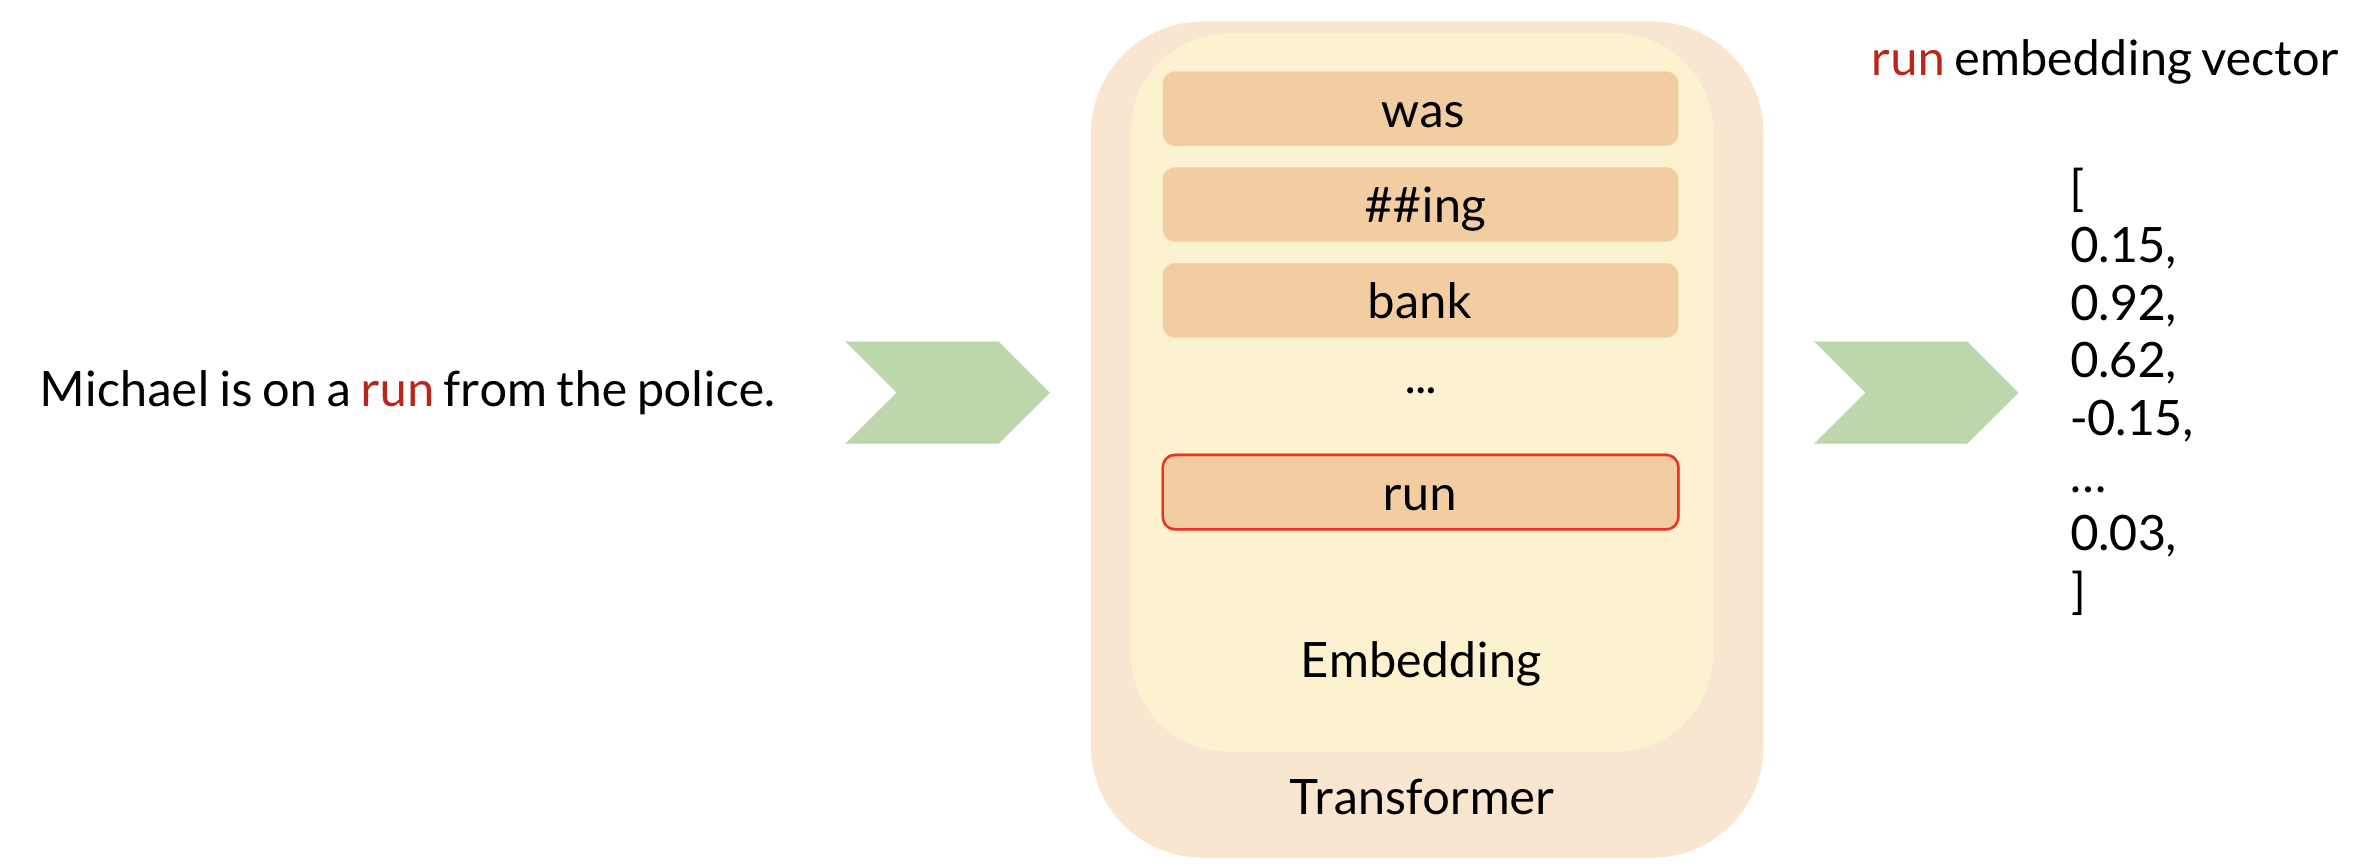
\includegraphics[width=\linewidth]{./assets/experiments/pipeline_vanilla_BERT.png}
  \caption{The BERT model takes as input a sentence $s$. The sentence $s$ is converted to a sequence of BERT tokens $t_1$, \ldots, $t_m$ using the WordPiece tokenizer.
Each item in the vocabulary $V$ has a corresponding embedding vector inside the embedding layer of the transformer.
This embedding vector is used by the intermediate layers of the transformer, and thus affects the downstream pipeline of the transformer for any subsequent layers of the transformer.
}
  \label{fig:BERT_vanilla_pipeline}
\end{figure}

%\begin{figure}[h]
%	\center
%  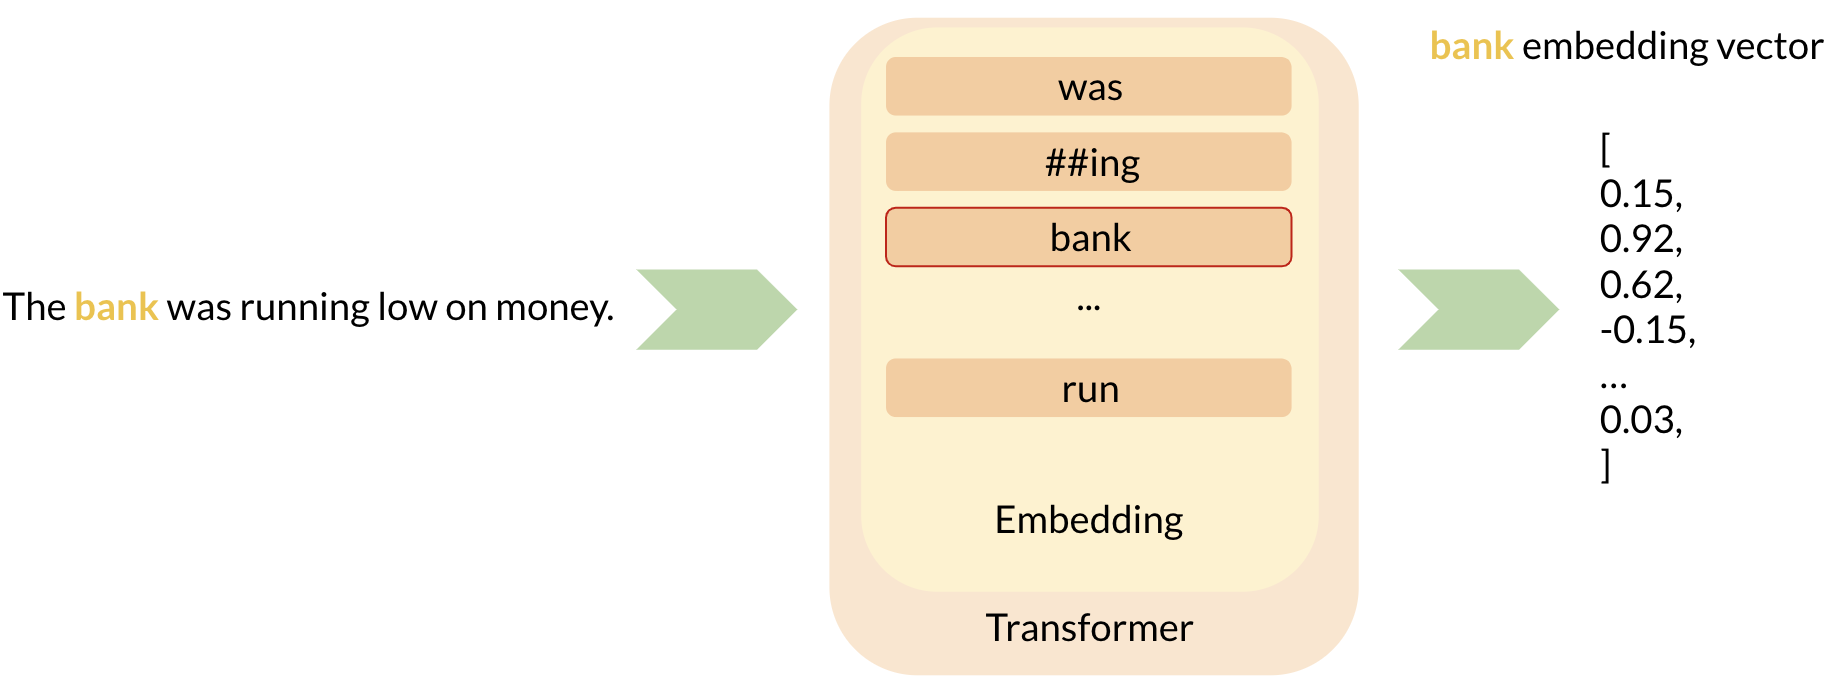
\includegraphics[width=\linewidth]{./assets/experiments/pipeline_tokenizer_BERnie_meaning_.png}
%  \caption{Figure similar to Figure \ref{fig:BERT_vanilla_pipeline}. this time, the targete word $w$ is \texttt{bank}.
%  }
%  \label{fig:BERT_vanilla_bank}
%\end{figure}

\subsubsection{Other language models}

Although we will only be working with the BERT language model in the subsequent sections, there is a wide variety of other language models using transformers.
These include GPT \cite{radford18} and GPT-2 \cite{radford19}, allowing the model to only consider the previous context (instead of the previous and subsequent context).
GPT and GPT-2 also include more fundamental modifications to the transformer module, most notably introducing layer normalization \cite{ba16} at various positions in the module. 
Other language models which extent BERT models include ALBERT \cite{lan20} - which is widely considered one of the state-of-the-art transformer models, DisilBERT \cite{sanh19}, HUBERT \cite{moradshahi19}, ERNIE \cite{sun19}, RoBERTa \cite{liu19}, SpanBERT \cite{joshi19} and StructBERT \cite{wang19d}.
Other lines of work compress representations produces by BERT \cite{shen19}, or interpret BERT as a markov random field \cite{wang19e}, formalizing the process of sampling sentences.

\section{GLUE benchmark dataset}

The GLUE benchmark dataset was first introduced by \cite{wang19}.
Please note that most state-of-the-art models achieve human-level accuracies for standard GLUE benchmarks, which is the reason \cite{wang19b} introduced SuperGLUE with even more advanced language tasks.
We will be using the standard GLUE benchmarking, as the basic BERT model does not out-perform human-level scores on this dataset.

\begin{figure}[h]
\center
\begin{tabular}{
 l % left aligned column
 l % left aligned column
 l
 l
 l
 l
 % *{2}{S[table-format=4.0]} % three columns with numeric data       
}
\toprule
\textbf{Corpus} & \textbf{ $|$Train$|$ } &\textbf{$|$Test$|$} & \textbf{Task} & \textbf{Domain}  \\
\midrule
%\multicolumn{6}{ c }{Helllo}
CoLA  & 8.5k  &  1k   & acceptability &  misc \\

SST-2 & 67k &  1.8k  & sentiment &  movie reviews \\

MRPC & 3.7k &  1.7k & paraphrase & news \\
          
STS-B & 7k &  1.4k    & sentence similarity &  misc. \\
      
QQP & 364k &  391k & paraphrase  &  social QA questions\\	

MNLI & 393k &  20k  & NLI  &  misc \\

QNLI & 105k &  5.4k & QA/NLI &  Wikipedia \\

RTE & 2.5k &  3k      & NLI &  news, Wikipedia \\

WNLI & 634 &  146   & coreference/NLI & fiction books \\

% SNLI & Accuracy &  0.8461 &              &  0.8367 \\
      
\bottomrule
\end{tabular}
\caption{Table taken from \cite{wang19}. Listing of all GLUE tasks including the linguistic phenomenon benchmarked, as well as the domain that the benchmarking data contains. Training and test set sizes are also provided.}
\end{figure}

We use an accuracy score for the majority of benchmarks. 
Some tasks have unbalanced classes or rank metrics, resulting in the F1-score or a correlation metric as the scoring function. 
The inference datasets are the most interesting tasks for us. 
Thus we will give a short outline of these benchmarking tasks. 
For a description on all other GLUE tasks, please refer to section \ref{appendix:GLUE} in the Appendix.

\subsubsection{Inference Tasks}

The Multi-Genre Natural Language Inference Corpus \textbf{MNLI} \cite{N18-1101} \cite{bowman2015} is a crowd-sourced collection of annotated sentence pairs for a textual entailment task.
For each premise and hypothesis sentence, the task is to predict whether the premise entails the hypothesis, contradicts the hypothesis, or does neither.
This is a 3-class classification problem.
The matched MNLI version tests on data which is in the same domain as the training set, while the mismatched MLNI tests on a training set which is cross-domain.
The MNLI data samples consist of parse-trees, which is the reason we do not display these here.
We will be working with the matched MNLI task only for convenience reasons.

The Stanford Question Answering Dataset is a question-answering dataset \cite{rajpurkar2016}. 
The authors of GLUE augment this dataset and create the Question answering Natural Language Induction \textbf{QNLI} benchmark, by relaxing the requirements that the model selects the exact answer, as well as the simplifying assumption that the answer is always present in the input and that lexical overlap is a reliable cue.
The task is to determine whether a context sentence contains the answer to the initially posed question. 

\begin{tcolorbox}
\begin{verbatim}
Who did the children work beside?	
In many cases, men worked from home.
not_entailment
\end{verbatim}
\end{tcolorbox}

\begin{tcolorbox}
\begin{verbatim}
How many alumni does Olin Business School have worldwide?
Olin has a network of more than 16,000 alumni worldwide.
entailment
\end{verbatim}
\end{tcolorbox}



The Recognizing Textual Entailment \textbf{RTE} consists of a series of annual textual entailment challenges. 
Data is combined from RTE1, RTE2, RTE3 and RTE5 \cite{dagan2005} \cite{bar2006} \cite{bentivogli2009} \cite{giampiccolo2007}. 
This is a classification task where the inputs are two sentences, and the models task is to predict one of the possible outputs \texttt{neutral}, \texttt{contradiction} and \texttt{no entailment}.

\begin{tcolorbox}
\begin{verbatim}
Oil prices fall back as Yukos oil threat lifted	
Oil prices rise.
not_entailment
\end{verbatim}
\end{tcolorbox}

\begin{tcolorbox}
\begin{verbatim}
Money raised from the sale go into Hepburn's family trust.
Proceeds go to Hepburn's family.	
entailment
\end{verbatim}
\end{tcolorbox}

The Winograd NLI \textbf{WNLI} dataset uses the original Winograd Schema Challenge dataset \cite{levesque2012}, which is a reading comprehension task where the model must read a sentence with a pronoun and select the referent of that pronoun from a list of choices. 
Sentence pairs are constructed by replacing the ambiguous pronoun with each possible referent.
The task is to predict if the sentence with the pronoun substituted is entailed by the original sentence.
The dataset includes adversarial examples which test negatively when overfitted.
Some example sentences include 

\begin{tcolorbox}
\begin{verbatim}
Bob was playing cards with Adam and was way ahead.
If Adam hadn't had a run of good luck, he would have won.	
Adam would have won.
label:0
\end{verbatim}
\end{tcolorbox}

\begin{tcolorbox}
\begin{verbatim}
Mark told Pete many lies, which Pete included in his book. 
He should have been more truthful.	
Mark should have been more truthful.
label:1
\end{verbatim}
\end{tcolorbox}


\section{WordNet}

The online lexical database WordNet was original introduced in \cite{miller90}.
WordNet is a semantic reference system similar but not identical to a thesaurus whose design is inspired by current psycholinguistic theories of human lexical memory.
English nouns, verbs and adjectives are organized into synonym sets, each representing one underlying lexical concept.
Different relations link the synonym sets.
The first version of WordNet contains of 95,600 different word forms (51,500 simple words and 44,100 collocations), and include a total of 70,100 word meanings, or sets of synonyms.
The authors argue that the rest of language is probably stored separately as part of the syntactic component of language.
The most ambitious feature of WordNet, however, is to attempt to organize lexical information in terms of semantics (word meaning).

The problem with alphabetical thesaurus is redundant entries. If Word $w_a$ and word $w_b$ are synonyms, the pair should be entered twice.
The problem with a topical thesaurus is that two look-ups are required, first on an alphabetical list and again in the thesaurus proper.
WordNet addresses these shortcoming through the concept of a \textit{lexical matrix}.

\paragraph{Lexical matrix:} 
The expression \textit{word} is often referred to both an utterance and to its associated concept.
\cite{miller90} specifies the difference between the two concepts as "word form", which refers to the physical utterance or inscription, and "word meaning", which refers to the lexicalized concept that a form can be used to express.
We will refer to \textit{semantics} whenever we mean \textit{word meaning}.

Figure \ref{fig:wordnet_table} depicts a lexical matrix, which encodes word-forms (columns), word-meanings (rows), and the existence of the possibility to express the word-meanings through the corresponding word-form (cell).
If multiple entries exist for a single column, then the single word-form encode multiple meanings, implying that the word-form is polysemous.
If multiple entries exist for a single row, the two words express the same underlying concept, and thus the two words-forms are synonyms.

\begin{figure}
\begin{center}
\begin{tabular}{ | c | c  c  c  c  c | } 
 \hline
 Word        &  &  & Word & Forms &  \\ 
 Meanings & $F_1$ & $F_2$ & $F_3$ & \ldots & $F_n$ \\ 
 \hline
 $M_1$     & $E_{1,1}$ & $E_{1,2}$ &  &  &  \\ 
 $M_2$     &  & $E_{2,2}$ &  &  &  \\ 
 $M_3$     &  &  & $E_{3, 3}$ &  &  \\ 
 $\vdots$ &  &  &  & $\ddots$ &  \\ 
 $M_m$    &  &  &  &  & $E_{m, n}$ \\ 
 \hline
\end{tabular}
\end{center}
\caption{Table taken from \cite{miller90}. Word-forms $F_1$, and $F_2$ are synonyms of each other, as they share one word meaning $M_1$. Word-form $F_2$, as it entails more than one meaning, namely $M_1$ and $M_2$.}
\label{fig:wordnet_table}
\end{figure}

WordNet refers to sets of synonyms as \textit{synsets}, which are a collection of word-forms that together determine a single meaning.
WordNet represents a semantic unit through such synsets.
WordNet is organized by semantic relations.
WordNet defines synonyms as a set of words, where one word is interchangable for another.
Because words in a synsets are interchangable due to their synonymous nature, WordNet organizes words into nouns, verbs, adjectives and adverbs, as the syntactic rules of language must also stay conform.

The authors mention that synonyms should be best thought of a continuum along which similarity of meaning can be graded.
However, through the introduction of synsets, the authors determine similarity in terms of a binary event, something which is either present, or not present.
The two tables \ref{fig:bank_synset} and \ref{fig:was_synset} show examples of how WordNet 3.1 introduces different semantic classes for the words \Verb#bank# and \texttt{was}.
We will make frequent use of WordNet, as it allows us to quantify semantics amongst word-forms.

\begin{figure}
\begin{center}
\begin{tabular}{ | c | p{11cm} | } 
 \hline
 Part of Speech & Definition \\  
 \hline
noun     & (sloping land (especially the slope beside a body of water)) "they pulled the canoe up on the bank"; "he sat on the bank of the river and watched the currents"\\ 
noun     & depository financial institution, bank, banking concern, banking company (a financial institution that accepts deposits and channels the money into lending activities) "he cashed a check at the bank"; "that bank holds the mortgage on my home" \\ 
 noun     & (an arrangement of similar objects in a row or in tiers) "he operated a bank of switches"  \\ 
verb & (tip laterally) "the pilot had to bank the aircraft" \\ 
verb    & (do business with a bank or keep an account at a bank) "Where do you bank in this town?"  \\ 
 \hline
\end{tabular}
\end{center}
\caption{Example output for WordNet 3.1 noun propositions for the word \texttt{bank}. In total, 18 different concepts are recorded.}
\label{fig:bank_synset}
\end{figure}

\begin{figure}
\begin{center}
\begin{tabular}{ | c | p{11cm} | } 
 \hline
 Part of Speech & Definition \\ 
 \hline
noun     & Washington, Evergreen State, WA, Wash. (a state in northwestern United States on the Pacific) \\ 
verb     & (have the quality of being; (copula, used with an adjective or a predicate noun)) "John is rich"; "This is not a good answer"
 bank"; "that bank holds the mortgage on my home" \\ 
 verb     & (an arrangement of similar objects in a row or in tiers) "he operated a bank of switches"  \\ 
verb & (form or compose) "This money is my only income"; "The stone wall was the backdrop for the performance"; "These constitute my entire belonging"; "The children made up the chorus"; "This sum represents my entire income for a year"; "These few men comprise his entire army" \\ 
verb    & (work in a specific place, with a specific subject, or in a specific function) "He is a herpetologist"; "She is our resident philosopher"  \\ 
 \hline
\end{tabular}
\end{center}
\caption{Example output for WordNet 3.1 noun propositions for the word \texttt{was}. In total, 14 different concepts are recorded.}
\label{fig:was_synset}
\end{figure}

\subsection{SemCor dataset}

The SemCor 3.0 corpus is an aggregation of the various Brown corpora \cite{francis64}, where each noun, adjective and verb is tagged with their respective ground-truth WordNet 3.0 sense.
SemCor was part of the early WordNet project, initially introduced in \cite{miller94}.
We provide some examples to give an idea of what the SemCor dataset looks like.
Looking at the example sentence

\begin{tcolorbox}
\begin{verbatim}
A Texas halfback who does n't even know the team 's plays,
 Eldon_Moritz, ranks fourth in Soutwest_conference scoring 
 after three games.
\end{verbatim}
\end{tcolorbox}

The corresponding part-of-speech labels are

\begin{tcolorbox}
\begin{verbatim}
DT, NN, NN, WP, VBZ, RB, RB, VB, DT, NN, 
POS, NN, NNP, VB, JJ, IN, NNP, VP, IN, JJ, NN
\end{verbatim}
\end{tcolorbox}

with the corresponding WordNet semantic class ids (for the first line only)

\begin{tcolorbox}
\begin{verbatim}
None, Texas.noun.0, halfback.verb.1, None, does.verb.6,
not.adverb.0, even.adverb.10, know.verb.1, None, team.noun.0,
is.verb.4, play.noun.14
\end{verbatim}
\end{tcolorbox}

\begin{figure}[h]
	\center
  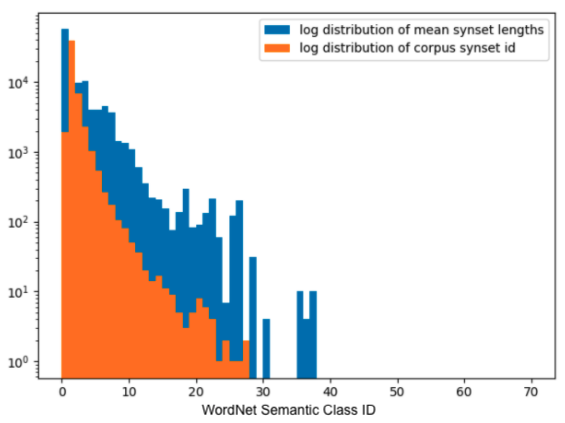
\includegraphics[width=0.6\linewidth]{./assets/background/semcor_skew.png}
  \caption{Shows that the SemCor data is biased towards words with low WordNet class IDs. 
  Words with a low WordNet sense index (i.e. close to 0) occur much more often than words that have a high WordNet sense index (i.e. above 5).
  The x-axis shows the WordNet sense index for a chosen word, while the y-axis shows the log-frequency within SemCor. 
  This is a cumulative plot over all words with WordNet senses within SemCor 3.0.
    There would be no bias if the two distributions would overlap.
  The skew could be a natural effect of how word lower WordNet indecies are assigned to more commonly used words.
  }
  \label{fig:embeddings_by_language}
\end{figure}


\chapter{Related Work}\label{section:RelatedWork} 

%TODO Add more structure
%TODO Organize by topics, not by papers ...

Previous work analyses to what extent language models capture sentiment, part-of-speech and semantics.
We will present a few relevant papers for each of these categories.

\section{Creating Synsets from Static Word Embeddings}\label{section_clustering}

\cite{pelevina16, biemann13, remus18, arefyev19, denkowski09} provide examples by which semantic embeddings or synsets are created using knowledge graphs or static word embeddings.

\cite{pelevina16, biemann13} use the Chinese Whispers algorithm initially proposed in \cite{biemann06} to cluster for synsets in word2vec vectors and the JoBimText framework \cite{biemann13} specifically.
\cite{denkowski09} uses 3-grams and creates a graph by drawing edges between words (nodes) that co-occur in the same phrase.
For static word vectors, an ego-network is created for each concept in the vector space whose correlation matrix $G(X)$ is the adjacency matrix for a resulting subgraph $\tilde{G}$

\begin{figure}[h]
	\center
  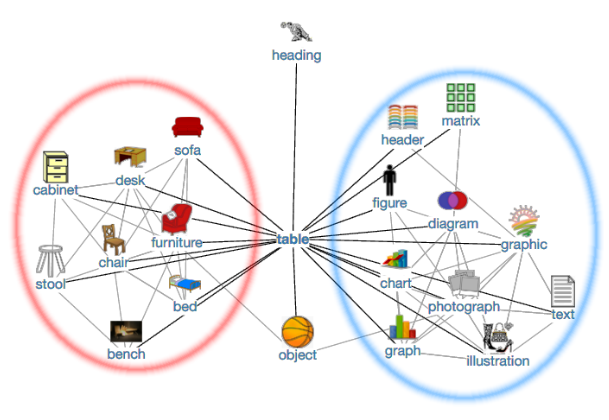
\includegraphics[width=0.6\linewidth]{./assets/relatedwork/ego_network.png}
  \caption{Figure taken from \cite{pelevina16}. An ego-network of the word \texttt{table} is created. Then, clustering is applied on the ego-network, to identify different semantic sets \textit{synsets}.}
  \label{fig:ego_network}
\end{figure}

Generalizing these approaches, one arrives at synsets as follows: 

\begin{enumerate}
\item Learn static word embeddings.
\item Build a graph of nearest neighbours based on vector similarities.
\item Cluster word senses using ego-network and applying the Chinese Whispers algorithm.
\item Aggregate the word-vectors with respect to the induced senses
\end{enumerate}

The biggest limitation lies in the word vectors or underlying data structure, as this already needs to capture the relevant information for clustering. \\

\begin{table}[H]
    \centering
    %\begin{tabularx}{\textwidth}{| X | X |}
    \begin{tabularx}{\textwidth}{p{50pt}|b}
    \toprule
      {\textbf{Vector}} & {\textbf{Nearest Neighbours}}  \\ \midrule
        table & tray, bottom, diagram, bucket, brackets, stack, basket, list, parenthesis, cup, trays, pile, playfield, bracket, pot, drop-down, cue, plate \\ \hline
        table\# 0 & leftmost\# 0 , column\# 1 , randomly\# 0 , tableau \#1 , top-left\# 0, indent\# 1, bracket\# 3, pointer\# 0 , footer\# 1 , cursor\# 1 , diagram\# 0 , grid\# 0      \\ \hline
        table\# 1 & pile\# 1, stool\# 1, tray\# 0, basket\# 0, bowl\# 1, bucket\# 0, box\# 0, cage\# 0, saucer\# 3, mirror\# 1, birdcage\# 0, hole\# 0, pan\# 1, lid\# 0    \\ \hline
    \end{tabularx}
\end{table}
\captionof{table}{Table taken from \cite{pelevina16}.
Neighbors of the word \texttt{table} and its senses produced.
The first row belongs to both senses, while the second and third row are distinct synsets.}

\cite{remus18} skip the clustering step and makes use of existing WordNet semantic class definitions, averaging the word vectors of synsets to arrive at synset vector representation.
Such methodologies prove to be useful in data-mining and document classification problems \cite{reimers19}.
Notice that if we have words that consist of multiple tokens, popular methods include applying a simple mean, max or min pooling over all token-embeddings (see \cite{bommasani19, akbik19, may19}) to arrive at a word-embedding. 
This is true for both contextual and static word embeddings. \\

\section{Quantifying word sense disambiguation}

Datasets have been proposed to benchmark word sense disambiguation performance for static word embeddings \cite{bruni13, hill15}.
\cite{pilehvar19} addresses the problem of a missing benchmark dataset for \textit{contextual word embeddings} to test contextual word embeddings for word sense disambiguation tasks.
The authors introduce the \textbf{Word in Context WiC} dataset of labelled sentence pairs, where the language model is supposed to learn the different semantic classes of a target word $w$. 
An example of this dataset includes (the first one with the target word \Verb#bed#, the second one with a target word \Verb#window#): \\

\begin{tcolorbox}
\begin{verbatim}
There's a lot of trash on the bed of the river.
I keep a glass of water next to my bed when I sleep.
label:False
\end{verbatim}
\end{tcolorbox}

\quad

\begin{tcolorbox}
\begin{verbatim}
The expanded window will give us time to catch the thieves.
You have a two-hour window of clear weather to finish work.
label:True
\end{verbatim} \\
\end{tcolorbox} 

A more extensive list of datasets separated by knowledge-based approaches and distributional-based approaches can be found in \cite{camachocollados18, liebeskind19, navigli19}.
Generally, it is assumed that occurrences in numerous different contexts implies polysemy.
\cite{camachocollados18} argues that about 80\% of all words in WordNet  3.0 are monosemous, with less than 5\% having more than 3 senses, underlining this property for practical effectiveness. \\

\section{Semantic subspace inside BERT}

There are mixed results when it comes to showing semantic structures in the contextual word embeddings produced by BERT.
We want to emphasize that most work deals with measuring the different between two distinct words $w_1 \neq w_2$, thus not always measuring phenomena such as polysemy. 

\subsection{Geometric analysis}

\cite{ethayarajh19, mickus19} use tools such as silhouette scores, and other measurements based on sampled contextual embedding vectors to draw conclusion on the semantic subspace of embedding vectors produced by BERT.

\cite{ethayarajh19} investigates the question of whether contextual word embeddings for a given word $w$ cover a closed area in the embedding space produced by BERT, or if there are infinitely many context-specific representations for each such word.
Models analyse include ELMo, BERT and GPT-2.
\cite{ethayarajh19} argues that in all models, contextual word embeddings are not isotropic, and thus not uniformly distributed with respect to direction.
Instead they are anisotropic, occupying a narrow cone in the vector space.
In GPT-2 alone, two randomly chosen words a cosine-similarity close to $1$.
For BERT, words in the same sentence grow more and more dissimilar in upper layers, but stay more similar to each other than randomly sampled vectors.
Finally, the SemCor corpus is used to calculate the following measures as indication for properties of how a semantic subspace is organized within BERT: \\

\begin{itemize}
\item \textit{self-similarity} of a word $w$ in layer $l$ is the average cosine similarity of word $w$ across $n$ different contexts as expressed by 
$$
\operatorname{SelfSim}_{\ell}(w)=\frac{1}{n^{2}-n} \sum_{j} \sum_{k \neq j} \cos \left(f_{\ell}\left(s_{j}, i_{j}\right), f_{\ell}\left(s_{k}, i_{k}\right)\right)
$$
\item \textit{intra-sentence similarity} is the similarity between the word-vector and the sentence-embedding, which is the mean of the token-embeddings for that sentence. 
Formally
$$
\begin{aligned} \operatorname{Intrasim}_{\ell}(s) &=\frac{1}{n} \sum_{i} \cos \left(\vec{s}_{\ell}, f_{\ell}(s, i)\right) \\ \text { where } \vec{s}_{\ell} &=\frac{1}{n} \sum_{i} f_{\ell}(s, i) \end{aligned}
$$
\item \textit{maximum explainable variance} is proportional to the variance in $w$ contextualized representations for a given layer.
It gives us an upper bound on how well a static word embedding could replace word's contextualized representations and is calculated by 
$$
\operatorname{MEV}_{\ell}(w)=\frac{\sigma_{1}^{2}}{\sum_{i} \sigma_{i}^{2}}
$$
where $\sigma_1, \ldots, \sigma_m$ are the first $m$ singular values of the occurrence matrix $
\left[f_{\ell}\left(s_{1}, i_{1}\right) \ldots f_{\ell}\left(s_{n}, i_{n}\right)\right]
$ where $f_l(s, i)$ maps word $w = s[i]$ in sentence $s$ to a contextual word embedding at layer $l$ of the language model.
\end{itemize}

%TODO Replace all "The author"

\quad

If both intra-similarity and self-similarity are low, then the model contextualizes words in that layer by giving each one a context-specific representation that is still distinct from all other word representations.
Low self-similarity implies a nuanced contextualization.
The authors conclude that all the language models considered are anisotropic in their sampled contextual word embeddings.
Due to this anisotropic property, the evaluations need to be adjusted for anisotropy, which can be done by subtracting the mean value for each formula across all words and at layer $l$. 
For BERT, the average cosine similarity between uniformly randomly sampled words is between $0.2$ and $0.6$, increasing with the number of layers.
This value would be close to 0 in a space where embeddings are isotropically distributed across the full vectorspace.
The authors argue that this is inherent to the process contextualization.
\cite{ethayarajh19} further show that stopwords, such as \texttt{the}, \texttt{of} and \texttt{to} to have the lowest self-similarity, implying that these have the most context-specific representations.
Although the authors argue that these words are not polysemous, it is apparent that these vectors are the ones with highest number of different contexts.
In the analysis it is shown that, language models do not simply assign one of a finite number of word-sense representations to each word, as this would lead to less variation in the representation.
Finally, \cite{ethayarajh19} takes the first principal component for each contextual word embedding (for different words $w_1, \ldots, w_N$) and benchmark this using tests designated for static word embeddings. 
They show that for layers 1 and 2 of BERT, these word-embeddings often outperform word sense disambiguation benchmarks.
\\

\cite{mickus19} analyses the structure inside BERT, and show that there is no strong correlation between the semantic feature of a word, and the location of the contextual word embedding produced by BERT.
Oddly, they find out that the position $i$ of the word $w_i$ inside the sequence $s = [w_1, \ldots, w_i, \ldots, w_T]$ has a stronger implication on the position of the produced contextual word embedding than the inputted word token does.
This is strongly manifested in contextual word embeddings with changing parity of the sentence position, i.e. when $w_i$ where $i$ is odd / even.
It is also mentioned that most papers that do an active analysis on this topic do not go enough into depth on the topic of the theory of meaning, but rather are trying to identify common patterns in modern language models.
The paper analyses these properties by conducting three experiments.
The first one is about \textit{word type cohesion}, which tests if similar words are projected into similar points in the contextual word embedding space.
\cite{mickus19} analyses if words with the same WordNet semantic class are projected to the same space inside BERT when sampled in different contexts.
They make use of the silhouette score \cite{rousseeuw87}, and a clustering scheme of words - where a cluster is defined by words in the same semantic classes.
Similar words are not projected to similar points in the context space.
The authors use the Wiktionary dictionary \cite{wiktionary} as an alternative to  semantic classes defined by WordNet.
They conclude that polysemous words result in degraded cohesion scores and decreased silhouette scores, and thus are more spread across the embedding space.
Despite all this, transformer-based LMs show great success of for downstream tasks.
Finally, \cite{mickus19} argues that the cosine similarity is a good distance measure for semantic similarity between contextual word embedding vectors, analogous to what was observed with static word vectors \cite{mikolov13}.
The authors continue with a sentence-pair similarity analysis, as well an analysis of the sentence-level structure, which is not of strong interest for our investigation. \\

We repeatedly find, that the correlation between certain linguistic features, such as part-of-speech and semantics, is not well noted when conclusions are drawn and examples are shown.

\subsection{Probing for semantics}

A \textit{probing task} refers to adding a (linear) modification to an underlying module (such as BERT), and then measuring performance for a downstream task.
This performance is used as an indication of how well the underlying module captures the concept scored by the task.

\cite{shi19, levine19, wiedmann19} revise modifications to BERT which allow BERT to predict sense labels or perform word sense disambiguation \textit{WSD} tasks. 
\cite{shi19} creates a relation extraction and semantic role labelling model using BERT as the underlying model.
The authors extend the BERT Model with a simple linear layer on top of the last hidden layer and use the CoNLL 2005 \cite{carreras04} as well as the 2012  dataset \cite{pradhan13} for labelled training, superseding prior non-BERT models with this simple BERT extension for the tasks of semantic role labelling. 
Similarly, \cite{levine19} revise a modification to BERT resulting in \textit{SenseBERT}.
This predicts not only the word-form of the masked words, but also the WordNet semantic classes (also called superenses).
A linear layer is appended on top of the final layer of BERT, making use of the final hidden representation.
Training is done in a supervised fashion using the SemCor dataset and the Word in Context \textit{WiC} task.

\begin{figure}
	\center
  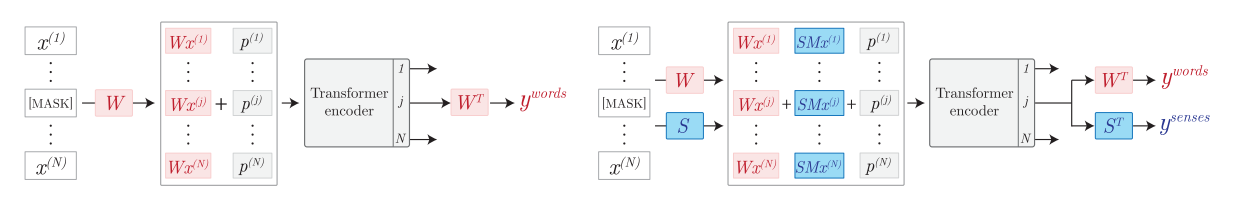
\includegraphics[width=\linewidth]{./assets/relatedwork/sensebert.png}
  \caption{Figure from \cite{levine19}. Standard BERT (left) and the SenseBERT adaptations (right), which include an embedding-encoder and an embedding-decoder specifically for WordNet senses.}
  \label{fig:embeddings_by_language}
\end{figure}

The authors record an up to 12\% gain in accuracy for in the SemEval-SS task (predicting SemCor WordNet labels), and up to 12\% improvement for the Word in Context task.
Even withouth fine-tuning, SenseBERT achieves competitive results with fine-tuned BERT.
The authors show that globally, these vectors seem to be properly aligned by their senses, even though they do not formally quantify this statement. \\

Alternatively \cite{wiedmann19} use a nearest neighbour classifier to measure the performance on  for two standard WSD benchmark datasets.
The authors show that BERT is able to put polysemic words into distinct 'sense' regions of the embeddings space, while ELMo and other models do not seem to possess this ability.
Prior work on using recurrent neural networks to classify sense labels exists \cite{kageback16}.
The authors argue that because for most NLP tasks, the fact that contextual word embeddings perform better implies that they also capture polysemy much differently.
The authors look at different contextual language models, including BERT and ELMo.
The distributional hypothesis includes that if the same word regularly occurs in different, distinct contextes, we may assume polysemy of its meaning \cite{miller91}.
The authors use the concatenation of the averaged wordpiece vectors of the last four layers as the contextual word embedding.

\begin{figure}[h]
	\center
  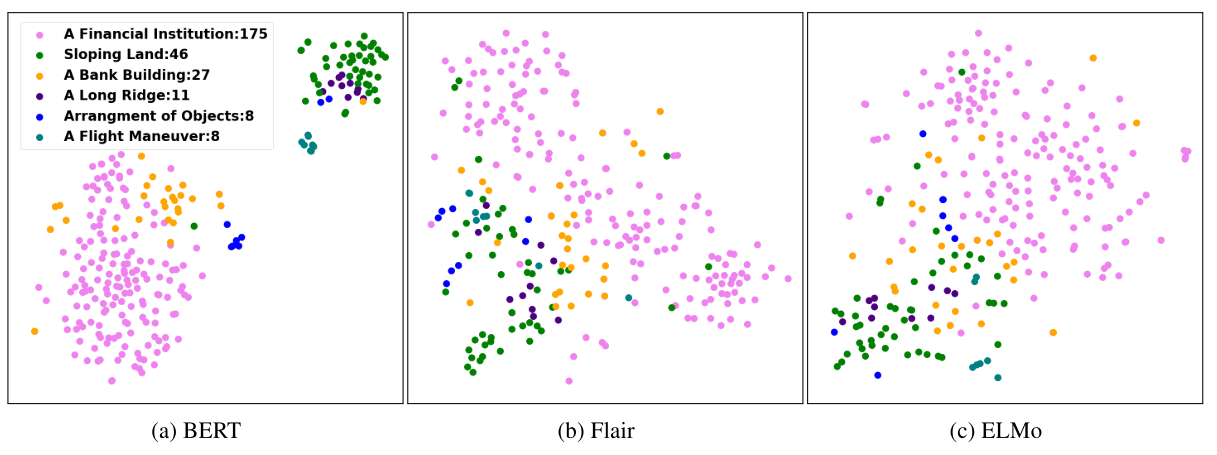
\includegraphics[width=0.9\linewidth]{./assets/relatedwork/wsd_bert.png}
  \caption{From \cite{wiedmann19}. T-SNE plots of different senses of \texttt{bank} and their contextual word embeddings. The legend shows a short description of the different WordNet sensees and the frequency of occurrence in the training data.
  }
  \label{fig:bert_wsd}
\end{figure}

The authors conclude that word-sense-disambiguation \textit{WSD} can be surprisingly effective using solely contextual word embeddings.
Different SensEval datasets are used for benchmarking, which also including SemCor. \\

\cite{coenen19} analyse semantic features qualitatively.
However, it is important to realize that the qualitative evaluation is not extensive, and only considers the linguistic feature of \textit{plurality}, and only on hand-picked examples.
Also, it is important to consider what causes the separation between clusters.
Given Figure \ref{fig:BERT_plurality}, one cannot reliably say that the part-of-speech feature \textit{causes} the partition into clusters.
\texttt{die} has different meanings when interpreted as a verb and as a noun, which could also be the reason the clusters are so strongly visible.

\begin{figure}[H]
	\center
  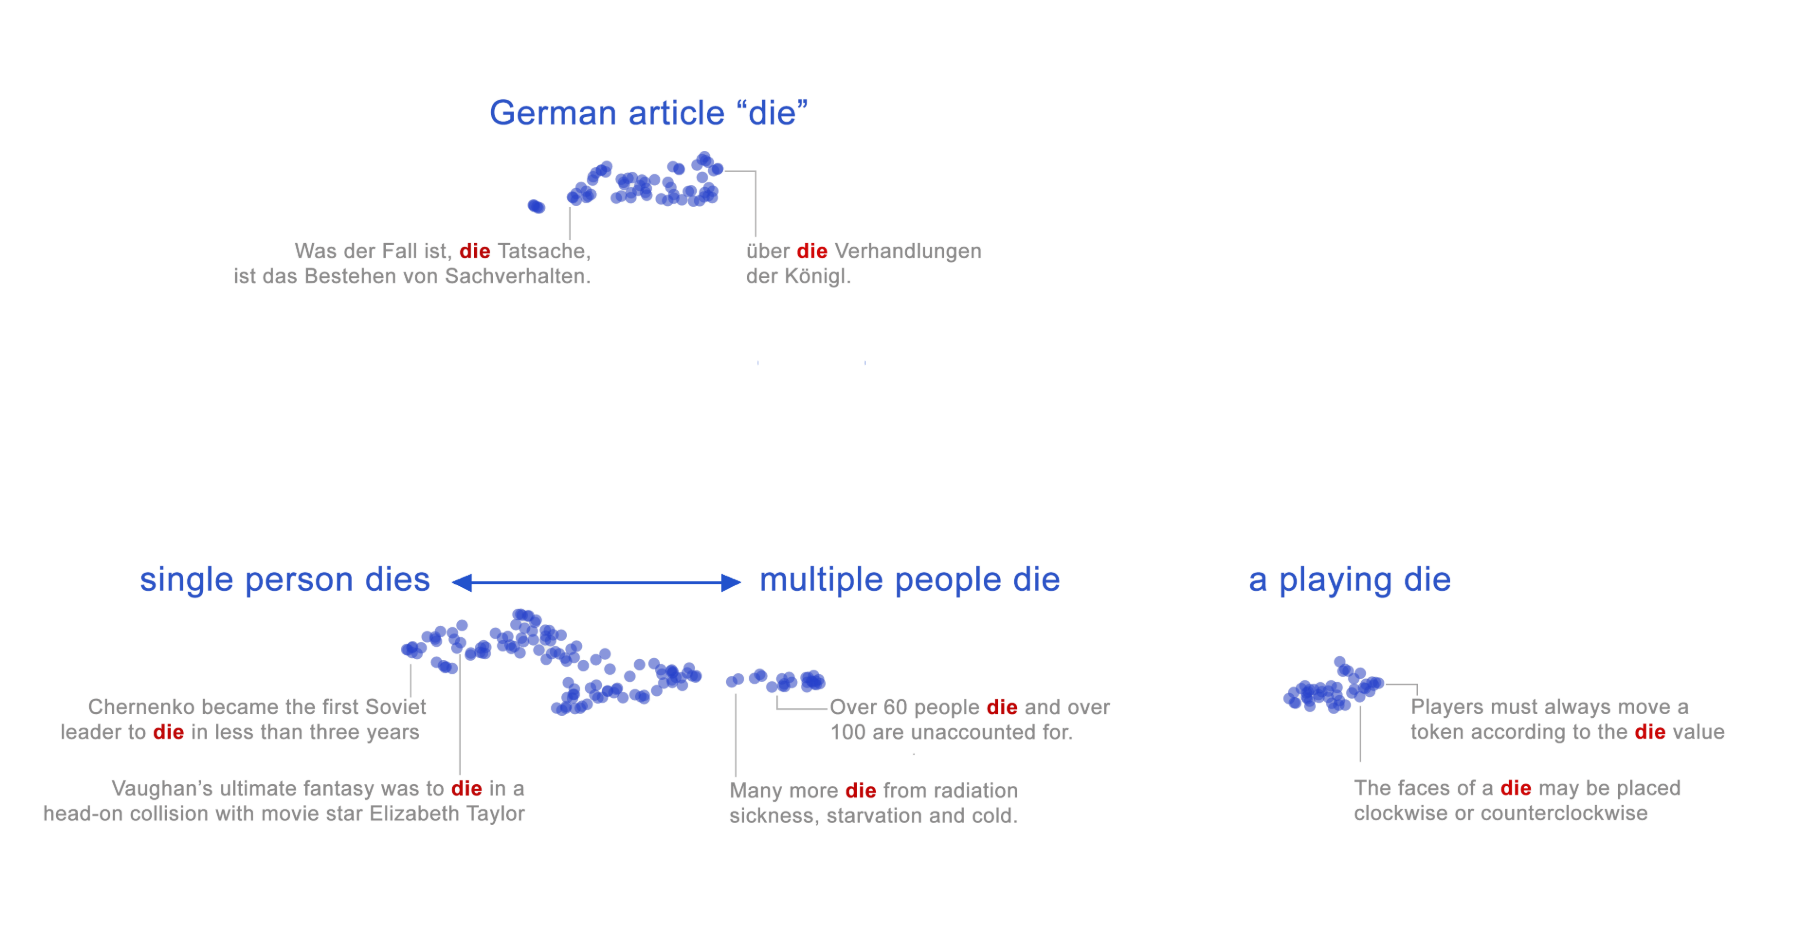
\includegraphics[width=0.9\linewidth]{./assets/relatedwork/BERT_plurality.png}
  \caption{From \cite{coenen19}. Embeddings for the word \texttt{die} in different contexts, visualized through UMAP. The blue text describes general annotations.
  Notice that in this case, the two semantic classes \texttt{die} also have two distinct part-of-speech tags.
  }
  \label{fig:BERT_plurality}
\end{figure}

A nearest neighbour classifier is built using the BERT embeddings resulting from the labelled SemCor corpus, achieving state-of-the-art results on this particular word-sense-disambiguation tasks.
The authors try to find a linear transformation matrix under which the word-sense-disambiguation task performs even better, however this results only in marginal benefit.
The underlying assumption is that the semantic features are encoded in an underlying subspace of the BERT context vectors.
In contrast to \cite{jawahar19}, \cite{coenen19} the authors also note that this suggests that more semantic information may be available in lower layers. \\

\subsection{Word sense disambiguation in specialized domains}

Semantic class prediction can be extended to other domains. 
For example, in the medical domain, different tokens can be interpreted as different medicines. 
\texttt{cold} can be interpreted as either a symptom, or temperature.
\cite{si19} use contextual word embeddings to better extract clinic concepts. 
Instead of WordNet semantic classes, medical entities are introduced, using medical datasets annotated with clinical concepts and amongst others, making use of BioBERT \cite{lee19}.
The authors demonstrate state-of-the-art results for clinical concept extraction. \\

\begin{figure}[H]
	\center
  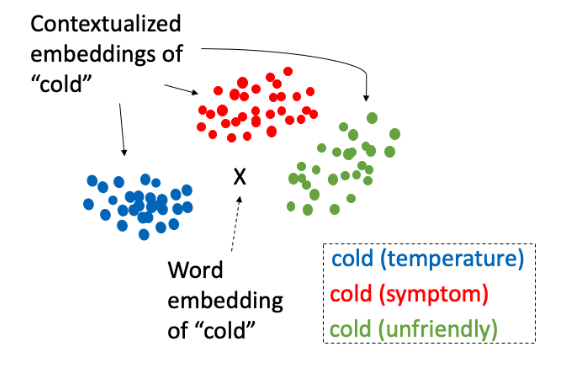
\includegraphics[width=0.4\linewidth]{./assets/relatedwork/cold_fictional_desired.png}
  \caption{Figure taken from \cite{si19}. \textbf{Fictional} embedding vector points and clusters of \texttt{cold}. This is one of the results that we want to arrive at.
  Specifically, we desire distinct word-embeddings that capture the modes of the underlying probability distribution. }
  \label{fig:cold_fictional_desired}
\end{figure}

\begin{figure}[H]
	\center
  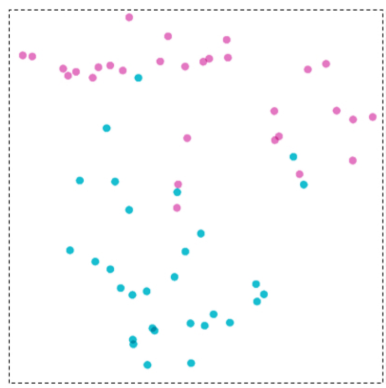
\includegraphics[width=0.3\linewidth]{./assets/relatedwork/cold_biobert.png}
  \caption{Figure taken from \cite{si19}. PCA visualizations using embedding vector of \texttt{cold} from BERT. The blue data points refer to \texttt{cold} as a temperature, whereas the red data points refer to \texttt{cold} as a symptom.}
  \label{fig:cold_fictional_desired}
\end{figure}


\section{Syntactic subspace in BERT}

Contextual word embeddings produced by BERT can also be analysed for syntactical properties.

\subsection{Extracting Parse-Trees}

\cite{coenen19, jawahar19} analyse how BERT encodes parse-trees in their attention mechanisms, and the distance between the produced contextual word embeddings. \\

\cite{coenen19} argue that on a high level, semantic and syntactic features seem to be present in different subspaces.
\cite{jawahar19} specifies this by arguing that BERT encodes surface features in bottom layers, syntactic features in middle layers, and semantic features in top layers.
\cite{coenen19} mention that there are fine-grained geometric representations of word senses, which is encoded in a relatively low-dimensional subspace.
However, this conclusion stems mostly from qualitative evaluation.
In slight contrast, \cite{jawahar19} cluster the representations (using normalized mutual information) at different layers $l$ of the model, and claim that lower layers encode phrasal information better, which is in slight contradiction to.
\cite{coenen19} use the Penn Treebank \cite{marcus93} to infer a dependency parsing scheme using a linear classifier with output of the transformer context vectors as input.
They achieve above 85.8\% accuracy for two-class classification, and 71.5\% accuracy for multi-class classification.
Prior work by \cite{hewitt19} finds that BERT encodes a parse tree where the tree distance seems to correspond to specifically to the square of the Euclidean distance.
A theorem is presented that shows that a tree with $n$ nodes has a Pythagorean embedding in $\mathbb{R}^{n-1}$.

\begin{figure}
	\center
  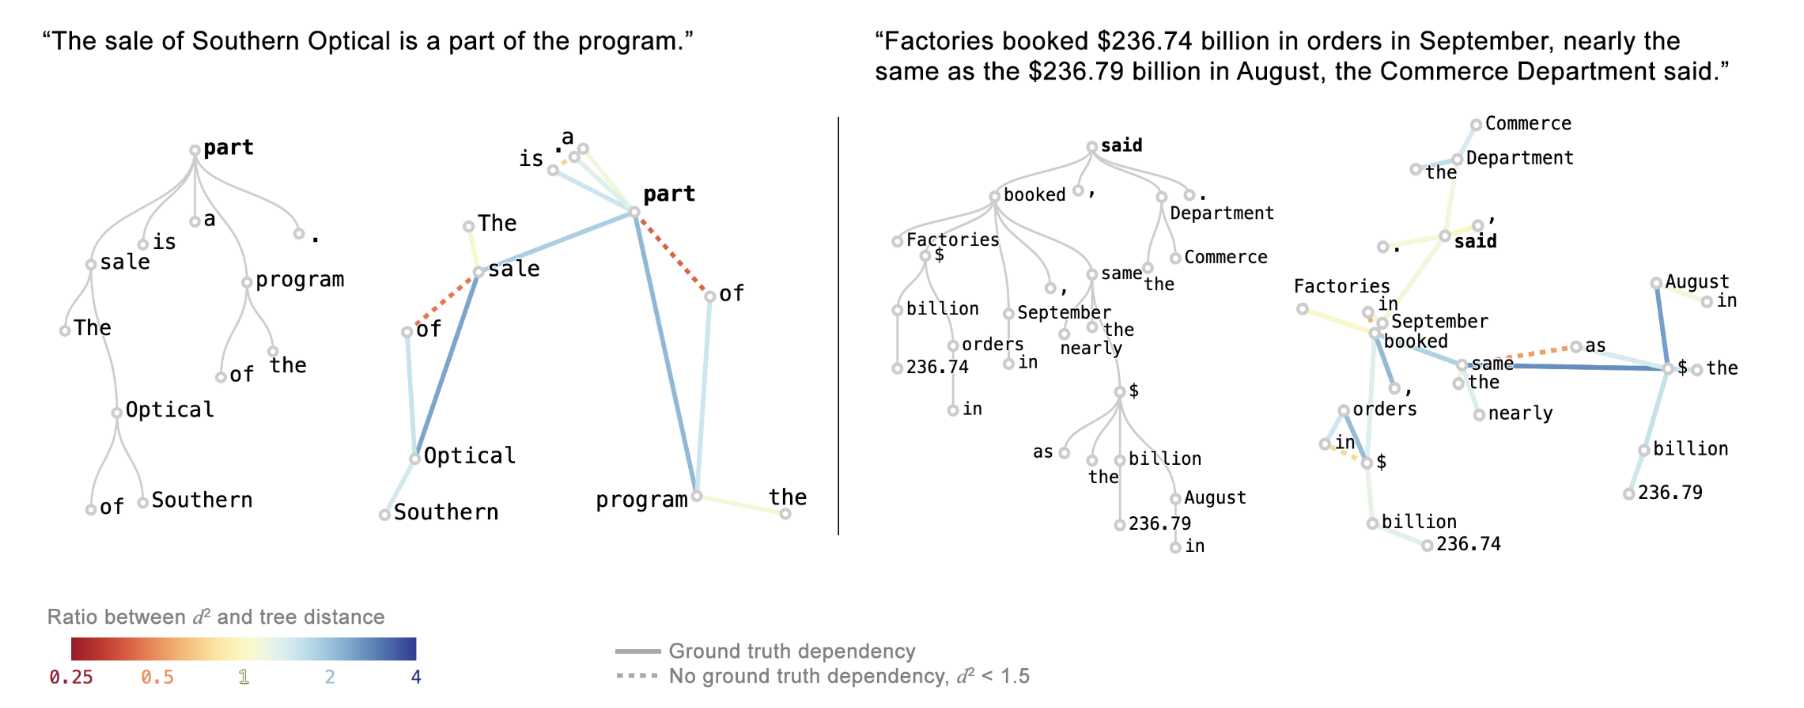
\includegraphics[width=\linewidth]{./assets/relatedwork/BERT_tree.png}
  \caption{From \cite{coenen19}. Visualizing the embeddings of two sentences after applying the Hewitt Manning probe. Parse tree (left) in comparison to the PCA projection of the contextual word embeddings (right). Small deviations are apparently, but an obvious resemblance exists. The color of an edge determines the squared Euclidean distance.}
  \label{fig:BERT_tree}
\end{figure}

\cite{jawahar19}  use a maximum spanning-tree approach to arrive at a dependency parsing tree extracted from the attention matrix depicted in Figure \ref{fig:parse_tree_jawahar}.\\

\begin{figure}
	\center
  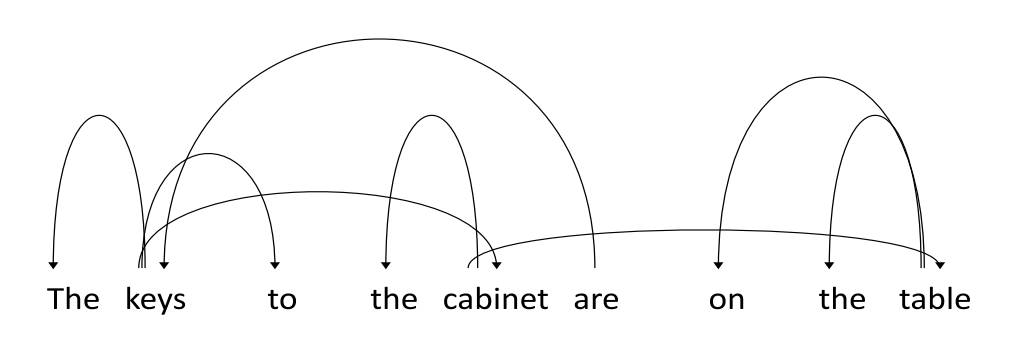
\includegraphics[width=0.7\linewidth]{./assets/relatedwork/BERT_dependency_parsing.png}
  \caption{From \cite{jawahar19}. Dependency parse tree induced from attention head in layer 11 in layer 2 using labelled root \texttt{are} as starting node with the maximum spanning tree algorithm}
  \label{fig:parse_tree_jawahar}
\end{figure}

\begin{figure}
	\center
  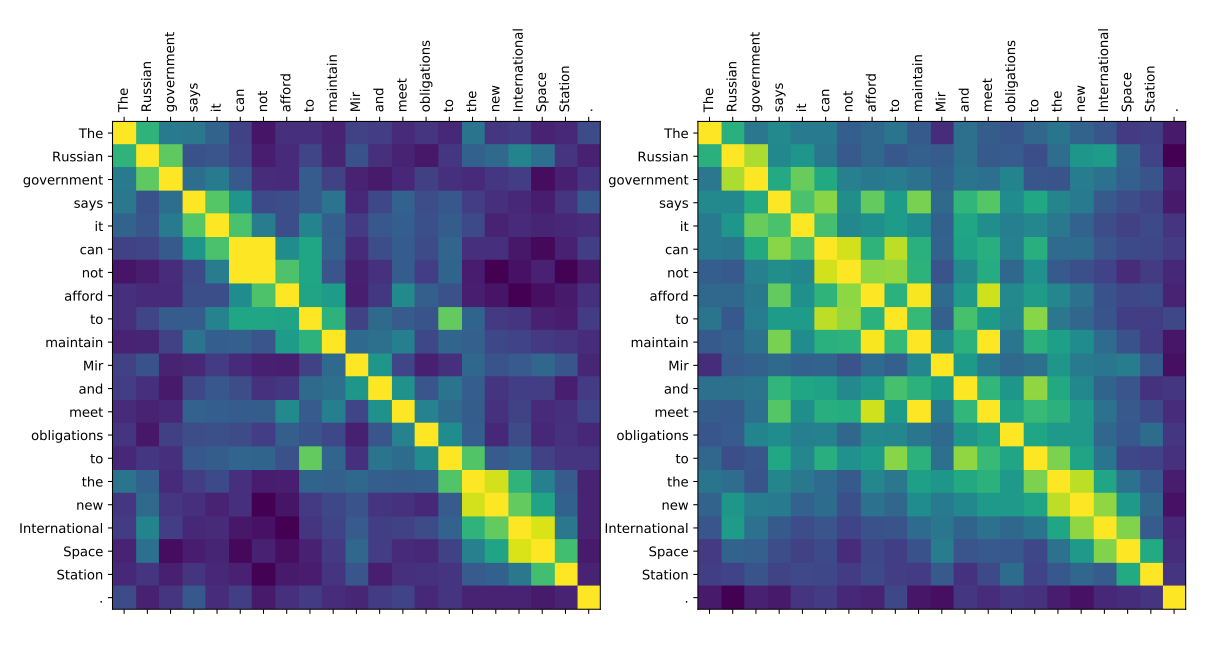
\includegraphics[width=0.9\linewidth]{./assets/relatedwork/self_attention_analysis.png}
  \caption{From \cite{peters18}. The authors show different similarity intensities (cosine similarity) between token-pairs using the output of a 4-layer LSTM (left), and the output after the first layer (right).}
  \label{fig:embeddings_by_language}
\end{figure}

\cite{peters18} do a similar analysis on a 4-layer deep LSTM-based language model. 
Similar to \cite{jawahar19}, they find that in general, lower layers mostly capture local information, while top layers represent longer range relationships, as the attention matrix has local spikes.
For bidirectional LMs, lower layers tend to place words from the same syntactic constituents in similar parts of the vector space.
The authors argue that in bidirectional LMs, semantics is captured only to a small extent, whereas morphology alone is most often used to answer questions on word analogy tasks.
The LM architectures learn syntax, as part-of-speech tags are captured at lower levels of the bidirectional LM layers.
The authors further build a contstituency parser with almost 80\% accuracy, by only adding a linear classifier and the span representation onto the lower layers of the bidirectional LMs.
A parse-tree is built using a greedy decoding step similar to \cite{joshi19b}. \\
 
\subsection{Subspace representing part-of-speech, verbs and arguments}

\cite{ribeiro19} aims to devise a verb-clustering and an argument-clustering approach which is supposed to devise a clustering that evokes frame-specific slots and thus semantic roles.
The authors again make use of the Chinese Whispers algorithm
\cite{biemann06} to arrive at the semantic frame cluster.
The authors use ELMo and BERT contextual word embeddings.
A graph is devised from the set of sampled contextual word embeddings $X$.
Edges all have the same weight, thus a cutoff function is defined by  which edges of lower weight (and thus lower similarity) are removed.

\begin{figure}[H]
	\center
  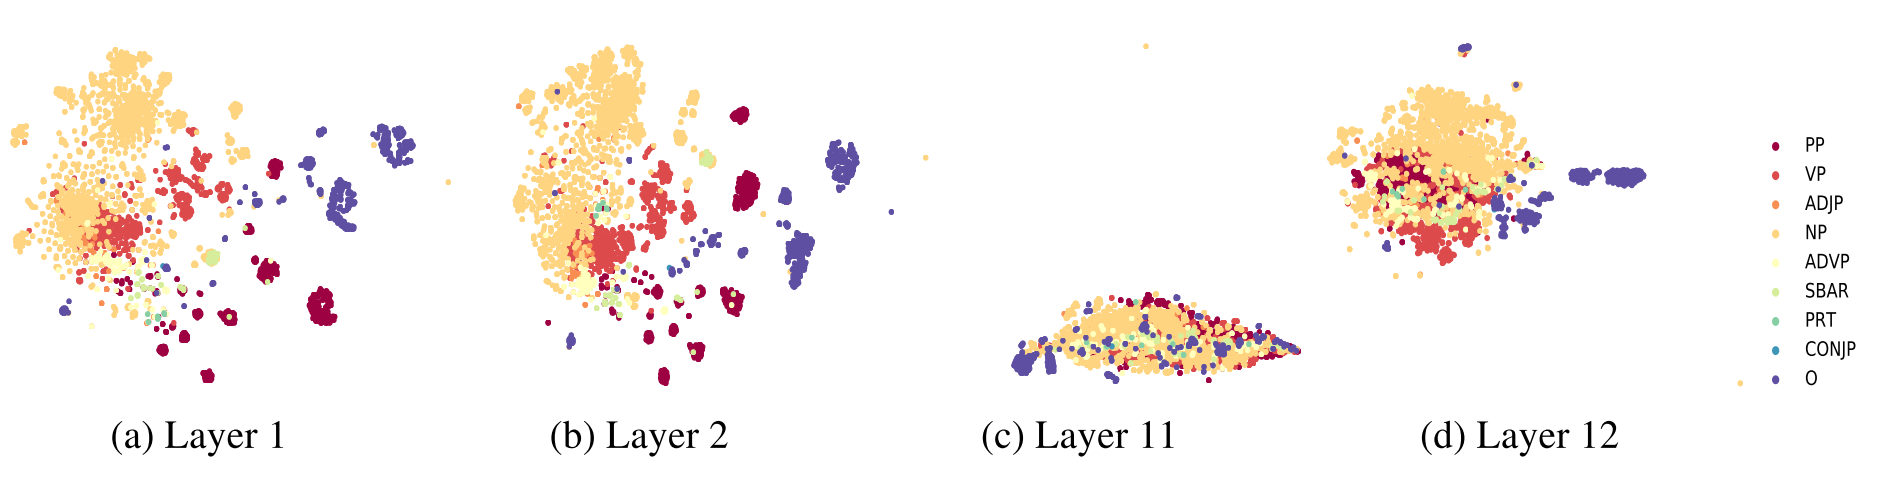
\includegraphics[width=0.9\linewidth]{./assets/relatedwork/BERT_tsne_layers.png}
  \caption{From \cite{jawahar19}. 2D t-SNE plot of span embeddings computed from the first and last two layers of BERT.}
  \label{fig:cold_fictional_desired}
\end{figure}

The cutoff function for the verb-clustering task is

\begin{equation}
t_f = \frac{\mu + \sigma}{2}
\end{equation}

where $\mu$ and $\sigma$ are the mean and standard deviation of the pairwise distance distribution, respectively. 
For argument clustering, the cutoff function used is defined as

\begin{equation}
t_a = \mu - 1.5 \sigma
\end{equation}

as a higher neighboring threshold is needed as the authors found out empirically.
Clustering performance is measured by the number of clusters found, and a purity metric which describes how homogenous the created clusters are. 
Labels from FrameNet \cite{baker98} are used for the homogenuity test. 
\cite{peters18} analyses the choice of different neural networks (i.e. LSTM, CNN or self-attention) and the effect it has on the underlying syntactical subspace produced. \\

Other lines of work includes models such as \textit{PAFIBERT} \cite{tan19}, which aims to transform sentences into a predicate-argument structure through additional modifications to BERT.
Implicitly, this solves a frame identification, as well as semantic role assignment task. \\

\section{Sentiment subspace in BERT}

Because context also implies sentiment, the context embeddings produced by BERT introduce a bias through the corpus that the LM was trained on.
Language models can also be used to evaluate how meaning and sentiment for certain words change over time.

\subsection{Bias} 

\cite{may19} measure social biases in BERT contextual word embeddings.
For this, they use static word embeddings by averaging over token-embeddings produced by BERT.
Although the authors cannot prove general trends, they show that certain suspicious patterns of sensitivity suggest that bias is occurring in different contexts.
Specifically, this is done by identifying relationships between concepts and attributes. 
\cite{may19, caliskan19} find that in the embedding space, concepts such as \texttt{European American names} are much more closely related to concepts such as \texttt{pleasant} than concepts such as \texttt{African American names}, which is a strong indication of bias.
\cite{caliskan19} follows a similar analysis, focusing much more on the properties of corpora used for training.
The authors hint that word-embeddings like word2vec also contain biases, where male names are more biased with career settings than female names. \\

\cite{may19} analyse the social biases that are part of the contextual word embeddings and show that depending on the language model (ELMo, BERT), the amount of social bias deviates. 
Because contextual word embeddings capture more than just semantics, bias is a natural implication of context vectors.
Although not very extensive on the topic of aggregation, the authors use techniques of mean-pooling, max-pooling, and last-pooling to arrive at a single context-vector, if the given token is intrinsically split-up by the language-model tokenizer (incl. BERT, ELMo, GPT).
Finally, evaluation on the corpora also yield inclusion of human-like biases \cite{jentzsch19} by names, races, male-vs-female. \\

\subsection{Change of language over time}

This bias can also be seen in how language changes over time. \cite{martinc20} looks at how language models capture the of change of meaning for different words over time.
The authors train language models on a balanced set of genres, from the 1960s and the 1990s.
The authors measure the variation coefficient of words.
The authors cluster the contextual word embedding spaces, and then calculate the drift measures through pearson and spearman correlations to arrive at a quantitative expression of how much language changes.
Similarly, \cite{hu19} quantitatively analyse how meaning changes using corpora from different historical epochs, including the 1890s, 1940s, 1960s, 1970s, 1990s and 2000s. 
Specifically, they show strong changes in static pairwise word-vector similarities when trained on differently epoched corpora.
They demonstrate through examples of the word \textit{gay} and \textit{alien} that the similarity between certain context-vectors change through time.

\chapter{How is semantics captured through contextual word embeddings produced by BERT?}\label{section:Understand_BERT}\label{section:UnderstandingBERT} 

In the previous section we have seen that although considerable work has been done in quantifying the syntactic subspace produced by BERT vectors, little work has been done in quantitatively evaluating the semantic nature of the outputs of BERT contextual word embeddings with respect to polysemy.
As such, we analyse BERT for how it organizes its semantic subspace for a given target word $w$.

We conduct three experiments.
The experiments have varying difficulty for the algorithm to understand the subspace organization for a given word $w$.
We start with a supervised algorithm which builds a discriminative model of the subspace, where labels are different semantic classes as defined by WordNet.
The second experiment aims to identify a similar subspace organization through an unsupervised algorithm, implicitly identify a multimodal structure within the subspace at which we look at.
Finally, we check how part-of-speech relates to semantics within the contextual word embeddings produced by BERT. 
This underlines the importance to distinguish between different linguistic features, especially when these are strongly correlated, something that has previously often led to premature conclusions (section \ref{section:RelatedWork}). 
This simplifies subsequent work.
It also helps explain the nature behind some visualizations in \ref{section:RelatedWork}.

\section{On the Linear Separability of meaning within sampled BERT vectors}\label{sec:linear_separability_experiment}

The first experiment takes as input a word of interest $w$ and samples a set of sentences $S$ from a corpus.
In this case, the above mentioned SemCor corpus and the news corpus \cite{news_corpus} which does not have any WordNet annotated classes are used.
To see if there is any structure within BERT vectors corresponding to the different meaning of one word, we ask ourselves whether or not different meaning are located at different extremes of the embedding space produced by BERT, or whether multiple semantic clusters form at different locations of the embedding space with the same WordNet semantic class label.
The latter scenario could occur as BERT is overparametrized \cite{kovaleva19}.
We test this hypothesis by training a linear classifier which learns a separating hyperplane between the different WordNet classes for $w$.
If a hyperplane exists with good separating accuracy, it is likely that different semantic concepts are located at different extremes of the embedding (sub-)space.

\subsection{Experiment setup}

To produce a contextual word embedding, we pass a sequence of words $[w_1, \ldots, w_i, \ldots w_T]$ sampled from $S$, where $w_i$ = $w$ (i.e. $w_i$ coincides with the word of interest) through the BERT model.
The output of BERT is a set of hidden representations which are interpreted as the contextual word embeddings $[x_{w_1}, \ldots, x_{w_i}, \ldots, x_{w_T}]$, where $x_{w_i}$ corresponds to the contextual word embedding of $w_i$.
This results in a feature matrix $X$ where each row corresponds to the sampled sentence when repeated $n$ times.
The columns correspond to the feature-dimensions of the contextual word embedding.
In all of our experiments, we set $n=500$, unless otherwise stated.
However, there are cases (especially for the SemCor dataset), where we cannot find $n$ sentences which include our word of interest $w$. 
In that case, we sample as many sentences as available in the corpus, making $n=min( S_{\text{available }w}, 500)$.
We make sure to conduct our investigation with words that occur often enough and take 30 occurrences per WordNet class as a lower cap.
Because this experiment requires $w$ to have multiple WordNet classes, we restrict the choice of $w$ to be polysemous as defined by WordNet.
Due to the restricted resources of SemCor, this limits our analysis to the following set of words \texttt{was}, \texttt{is}, \texttt{be}, \texttt{are}, \texttt{more}, \texttt{one}, \texttt{first}, \texttt{only}, \texttt{time}.
Although these words are not the most intuitive polysemous words (as would \Verb#bank# be, for example), the limited "obviousness" should allow this experiment to reject the hypothesis less easily.
To work with similar input to the classification algorithms, we apply a standard scalar such that the input data $X$ is normalized around $0.0$ with standard deviation $1.0$.
We also test if dimensionality reduction techniques improve the performance.
The reason for this is to have a stricter set of requirements for the separating hyperplane to be drawn.
If the dimensionality of the data $d$ is high, but the number of samples $n$ is low, then the system of linear equations is underdetermined, as there is an infinite set of hyperplanes in the solution space.
Projecting $X$ to a lower dimensionality works like a regularizer. This restricts the set of candidate hyperplanes.
On a separate note, this also tests if the semantic notion of the context vectors is kept at a lower dimension using a simple model such as PCA.
In summary, the experimental setup is captured through algorithm \ref{alg:linear_separability}. \\

\begin{algorithm}[H]
\SetAlgoLined
\SetKwInOut{Input}{Input}
\Input{A target word $w_{\text{target}}$; The latent dimensionality $k$ for PCA;}
\KwResult{Accuracy of a logistic regression classifier}
 $\mathbf{D}, \mathbf{y} \leftarrow $  sample up to 500 sentences (as much as available) from the SemCor corpus which include the word $w_{\text{target}}$, along with the corresponding WordNet meaning-id\;

$ \mathbf{X} \leftarrow BERT( \mathbf{D} )$ i.e. pass each sentence through BERT and retrieve the resulting contextual word embedding $x_w$ as defined in the above section\;
 
$ \mathbf{X}, \mathbf{y} \leftarrow oversample( \mathbf{X}, \mathbf{y} )$ such that we don't have dominating classes\;
 
$ \mathbf{X_\text{train}}, \mathbf{X_\text{test}}, \mathbf{y_\text{train}}, \mathbf{y_\text{test}} \leftarrow trainTestSplit( \mathbf{X}, \mathbf{y}, testProportion=0.4 )$ \;

$ \mathbf{X_\text{train}} \leftarrow StandardScaler( \mathbf{X_\text{train}})$ such that all the data is normalized\;

$ \mathbf{X_\text{train}} \leftarrow PCA( \mathbf{X_\text{train}}, k )$ such that all the data is projected to a lower latent dimensionality $k$\;

$ model \leftarrow LogisticRegression( \mathbf{X_\text{train}}, \mathbf{y_\text{train}} )$ \;
    
$ \mathbf{\hat{y}_\text{test}} \leftarrow model.predict(\mathbf{X_\text{test}})$ \;

$ accuracy, confusionMatrix \leftarrow loss(\mathbf{y_\text{test}}, \mathbf{\hat{y}_\text{test}}) $ \;
    
return $ accuracy, confusionMatrix $\;
    
 \caption{Checks sampled BERT vectors for linear interpretability by meaning}
 \label{alg:linear_separability}
\end{algorithm}

\hfill \break

We use standard the sklearn \cite{scikit-learn} implementations for the Standard Scalar, PCA and Logistic Regression. 
We use the Hugginface transformers library \cite{Wolf2019} for the  BERT model, and also all subsequent modification of BERT.
The loss function we use is the $l1$ loss function, where the loss for a correct sample is $0$, and for an incorrect class assignment is $1$.
We apply 5-fold cross validation and measure the mean accuracy as well as the standard deviation of the accuracy. 
We also note the variance kept after projecting PCA on the lower dimensionality $k$ to understand how a simple dimensionality reduction technique can affect the separation between semantic classes.

\subsection{Results}

We run the above experiment for a set of different $k$. 
The variance shown below is a fraction of $1$. 
A "variance kept" value of $1$ corresponds to no information loss in terms of eigenvalues left out.

We show the result for three candidate experiments, for the words \Verb#was#, \Verb#is# and \Verb#one# respectively, as these are the words that have the highest number of occurrences within the 
SemCor dataset.
In high dimensions, there are many possible separating hyperplanes due to candidate model space growing exponentially with the number of dimensions.

\begin{center}
\captionof{table}{Mean and standard deviation of the accuracy of a linear classifier trained on the 2 most common classes of WordNet meanings for the word \textit{was}.}
\begin{tabular}{SSSSSSSS} \toprule
    {dimensionality} & {variance kept} & {accuracy (mean / $\pm$ stddev)}  \\ \midrule
     10  & 0.27 & 0.82 / $\pm$ 0.03 \\ \midrule
     20  & 0.41 & 0.81 / $\pm$ 0.04  \\ \midrule
     30  & 0.50 & 0.85 / $\pm$ 0.03  \\ \midrule
     50  & 0.63 & 0.92 / $\pm$ 0.03 \\ \midrule
     75  & 0.73 & 0.94 / $\pm$ 0.02 \\ \midrule
    100 & 0.81 & 0.95 / $\pm$ 0.02  \\ \midrule
\end{tabular}
\end{center}

% -> show which two different word meanings are sampled

% Also perhaps show the confusion matrix

\begin{center}
\captionof{table}{Mean and standard deviation of the accuracy of a linear classifier trained on the 2 most common classes of WordNet meanings for the word \textit{is}.}
\begin{tabular}{SSSSSSSS} \toprule
    {dimensionality} & {variance kept} & {accuracy (mean / $\pm$ stddev)}  \\ \midrule
       2  & 0.09 & 0.57 / $\pm$ 0.02 \\ \midrule
     10  & 0.29 & 0.82 / $\pm$ 0.03  \\ \midrule
     20  & 0.42 & 0.82 / $\pm$ 0.04  \\ \midrule
     30  & 0.51 & 0.83 / $\pm$ 0.03  \\ \midrule
     50  & 0.72 & 0.85 / $\pm$ 0.04 \\ \midrule
     75  & 0.78 & 0.84 / $\pm$ 0.04 \\ \midrule
    100 & 0.79 & 0.85 / $\pm$ 0.03  \\ \midrule
\end{tabular}
\end{center}

% -> show which two different word meanings are sampled
\quad

\begin{center}
\captionof{table}{Mean and standard deviation of the accuracy of a linear classifier trained on the 2 most common classes of WordNet meanings for the word \textit{one}.}
\begin{tabular}{SSSSSSSS} \toprule
    {dimensionality} & {variance kept} & {accuracy (mean / $\pm$ stddev)}  \\ \midrule
       2  & 0.10 & 0.55 / $\pm$ 0.10 \\ \midrule
       3  & 0.14 & 0.51 / $\pm$ 0.05 \\ \midrule
     10  & 0.34 & 0.59 / $\pm$ 0.08  \\ \midrule
     20  & 0.50 & 0.76 / $\pm$ 0.03  \\ \midrule
     30  & 0.62 & 0.77 / $\pm$ 0.02  \\ \midrule
     50  & 0.76 & 0.83 / $\pm$ 0.06 \\ \midrule
     75  & 0.87 & 0.87 / $\pm$ 0.05 \\ \midrule
    100 & 0.94 & 0.87 / $\pm$ 0.05  \\ \midrule
\end{tabular}
\end{center}

\hfill \break

\begin{center}
\captionof{table}{Mean and standard deviation of the accuracy of a linear classifier trained on the 4 most common classes of WordNet meanings for the word \textit{was}.}
\begin{tabular}{SSSSSSSS} \toprule
    {dimensionality} & {variance kept} & {accuracy (mean / $\pm$ stddev)}  \\ \midrule
       2  & 0.08 & 0.38 / $\pm$ 0.03 \\ \midrule
       3  & 0.11 & 0.38 / $\pm$ 0.04 \\ \midrule
     10  & 0.28 & 0.65 / $\pm$ 0.03  \\ \midrule
     20  & 0.43 & 0.76 / $\pm$ 0.04  \\ \midrule
     30  & 0.53 & 0.83 / $\pm$ 0.03  \\ \midrule
     50  & 0.67 & 0.93 / $\pm$ 0.01 \\ \midrule
     75  & 0.77 & 0.95 / $\pm$ 0.01 \\ \midrule
    100 & 0.83 & 0.95 / $\pm$ 0.01  \\ \midrule
\end{tabular}
\end{center}

\hfill \break

We get very similar accuracies for \Verb#time#, \Verb#made#, \Verb#thought#.
However, these tables are left out as we do not deem these to be statistically significant due to limited sample sizes.
To make sure that no inconsistencies happen during testing, we also analyse the confusion matrices, which all were balanced across class-pairs.
The transpose elements were usually off by only 1-4 samples, and the majority of the samples were correctly predicted (and thus on the diagonal of that matrix).
The reader can see that for a learned hyperplane, the classification accuracy reaches more than 75\% for dimensions of more than 20.
This is also the case for multiclass classification problems, which removes the possibility that overfitting could have occurred at low dimensions.

\section{On the Clusterability of meaning within sampled BERT vectors} \label{experiment_BERT_clusterability}

Modality-detection can tell us a lot about the nature of a dataset.
It can tell us what the predominant categories of a dataset are.
Given a set of clusters amongst vectors $x_1, \ldots, x_n$ organized in a matrix $X$, the different clusters can be interpreted as the different modes of the data.
The key takeaways follow a similar interpretation as what principal components are, showing us the features and latent dimensions with greatest differences.
Investigating the difference between clusters can show us how different classes are different from each other.

There are different ways to check if a set of vectors is clusterable. This includes theoretical ways to determine clusterability, for example as described in \cite{ackerman09, mccarthy16}. 
However, we are most interested in the practical clusterability of BERT, and as such, we decide to follow a brute-force approach to find clusters within BERT. The experiment on linear separability has shown us that different semantically annotated samples are at different locations of the embedding space.
We now want to investigate how easily this clustering can be found, and if the transitioning between the semantic categories is a smooth transition, or constitutes a hard partitioning between context vectors.

\subsection{Experiment setup}

In section \ref{sec:linear_separability_experiment}, we try to train a discriminative model.
Now we try to come up with a quasi-generative model which is able to detect modalities of the underlying true distribution, which in theory could be used to generate new data samples.
Consequently, this task is a more difficult problem than finding a separating hyperplane as done in section \ref{sec:linear_separability_experiment}. 

One of our goals is to identify semantic clusters within a given set of contextual word embeddings.
Implicitly, this requires the algorithm to solve a multi-modality detection problem.
This means that we cannot use algorithms such as k-means \cite{lloyd57, macqueen67}, as this requires the number of clusters to be known prior to running the algorithm.
Instead, we turn our attention to algorithms, which both find clustering assignments and also the best number of clusters that the data can be clustered by.
Although we could also include more complex models such as autoencoders or other neural network based algorithms in this analysis, we decide to focus on popular and non-parametric algorithms outside the domain of neural networks.
Please refer to section \ref{appendix:Clustering} in the Appendix for an intuitive description of how of the algorithms we use work, as we assume that the reader is familiar with algorithms such as DBScan, Affinity Propagation and MeanShift. \\

Initially, we tried to cluster the matrix of embedding vectors $X$ using standard approaches with no hyperparameter optimization. 
However, all of the algorithms we applied would fail with the default hyperparameters, indicating that no clustering can be found.
We suspect that this is the case as the vectors produced by BERT seem to be smoothly distributed across the span of $X$, as can be seen in the PCA visualizations. \\

As such, we had to adapt our experiment setup and implement an efficient hyperparameter selection tool, making use of random search and \cite{bergstra12} and Bayesian optimization \cite{wang13}.
We use the Pytorch Adaptive Experimentation platform \cite{pyax} which automatically chooses which of the two policies to use, given the dimensionality and number of parameters to search for.
Specifically, our experiment setup is precisely described by the algorithms \ref{alg:cluster_low_level} and \ref{alg:hyperparameter}.
Algorithm \ref{alg:cluster_low_level} calculates the clustering overlap between the predicted clustering $\hat{y}$ and the true cluster labels as defined by the WordNet semantic class labels $y$.
The input to this algorithm is the clustering model that we want to use including the Chinese Whispers algorithm (\ref{section_clustering}). 
We optionally reduce the dimensionality of the input embeddings through either PCA, or UMAP.
Finally, we provide the target word $w$ for which we want to calculate this overlap score.

Similar to \cite{pelevina16} our goal is to cluster contextual word embeddings.
However, we have to modify the Chinese Whispers algorithm as \cite{pelevina16} applies this for static word embeddings and we are utilising BERT contextual word embedding.
Our modified version of the Chinese whispers is described in Algorithm \ref{alg:cluster_high_level}. \\

\begin{algorithm}[H]
\SetAlgoLined
\SetKwInOut{Input}{Input}
\Input{
$X$: The set of contextual word embeddings for a word $w$ included in a set of $n$ sentences. 
These are the BERT vectors we want to cluster; \\ 
}
\KwResult{Cluster assignments for each of the samples within $X$.}

corMatrix = cosineSimilarity(X, X) \\
closestNeighbors = argsort(corMatrix, axis=1)[:, :n] \\
corMatrix[not in closestNeighbors] = 0. \\

corMatrix[identifyHubs(corMatrix)] = 0. \\

clusters = runChineseWhispersOnGraph(corMatrix) \\

clusters = extrapolateHubsByNearestNeighbors(clusters) \\

return clusters

 \label{alg:cluster_high_level}
 \caption{Checks sampled BERT vectors for clusters by  meaning}
\end{algorithm}

\hfill \break

Intuitively we create an adjacency matrix \texttt{corMatr} for a graph $G$ from the set of vectors $X$ using the following algorithm, which is then passed on for clustering to the \texttt{RunChineseWhispersOnGraph} algorithm using the NetworkX implementation \cite{hagberg04}.
Compared to static word embeddings, contextual word embeddings suffer of the \textit{hubness property} \cite{conneau17} for a variets of tasks.
The hubess property describes that there are certain embeddings (called hubs), which in the high-dimensional space are connected to a majority of other embedding vectors.
This leads to the Chinese Whispers algorithm to collapse onto a single cluster assignment for the entire dataset.
To improve performance and addresses the hubness problem mentioned in \cite{conneau17} we identify hubs by the following cutoff formula.

\begin{equation}
\texttt{cutoff}(x) = \mu ( X ) + c \sigma (X)
\end{equation}

where $c$ is an adjustable hyperparameter.
These hubs are removed if the connectivity value is too high. \\
%TODO END OF MODIFICATION TODO

\begin{algorithm}[H]
\SetAlgoLined
\SetKwInOut{Input}{Input}
\Input{
$w_{\text{target}}$: The target word whose BERT vectors we want to cluster; \\ 
$DimRed$: The dimensionality reduction method; \\
$k$ : The latent dimensionality for the dimensionality reduction method; \\ 
$ClusterAlgorithm$: The clustering algorithm to use;
}
\KwResult{The associated cluster-id with each sampled sentence, and the adjusted random index.}

 $\mathbf{D}, \mathbf{y} \leftarrow $  sample up to 500 sentences from the SemCor corpus which include the word $w_{\text{target}}$, along with the corresponding WordNet meaning-id, and compensate more sentences by sampling from the news corpus if less than 500 sentences are available in the SemCor sentence.
We set y = -1 whenever no labeling information is available, which is the case if we don't sample data from the SemCor corpus.\;

$ \mathbf{X} \leftarrow BERT( \mathbf{D} )$ i.e. pass each sentence through BERT and retrieve the resulting contextual word embedding $x_w$ as defined in the above section\;
 
$ \mathbf{X}, \mathbf{y} \leftarrow oversample( \mathbf{X}, \mathbf{y} )$ such that we don't have dominating classes (all except for $y = -1$).\;
 
$ \mathbf{X} \leftarrow StandardScaler( \mathbf{X})$ such that all the data is normalized\;

$ \mathbf{X} \leftarrow DimRed( \mathbf{X}, k )$ such that all the data is projected to a lower latent dimensionality $k$\;

$ model \leftarrow ClusterAlgorithm( \mathbf{X})$ \;

$ \mathbf{\hat{y}} \leftarrow model.predict(\mathbf{X}) $ \;

$ score \leftarrow AdjustedRandomIndex(\mathbf{\hat{y}[semcor]}, \mathbf{y[semcor]}) $ \;

return $ score, \mathbf{\hat{y}}$\;
    
 \caption{Checks sampled BERT vectors for clusters by  meaning}
  \label{alg:cluster_low_level}
\end{algorithm}

\hfill \break

Running this over all possible clustering algorithms, and taking the mean across a set of words, we get a reliable estimate of which clustering approach generalizes best across words.
This is depicted in the algorithm \ref{alg:cluster_hyperparameters}.

\begin{algorithm}[H]
\SetAlgoLined
\SetKwInOut{Input}{Input}
\Input{
$w_{\text{target}}$: The target word whose BERT vectors we want to cluster; \\
}
\KwResult{The model which has the highest adjusted random index score between its predicted clustering, and the true underlying clustering as given by the SemCor WordNet class labels.}

\textbf{for} clusterModelClass in clusterModels:  \\
\quad \quad \textbf{for} modelConfiguration \textbf{in} clusterModelClass.hyperparNext() :  \\
\quad \quad \quad \quad \textbf{for} $w$, $X$, numberOfSenses, trueClustering, knownIndices \\
\quad \quad \quad \quad \textbf{in} crossvalidationDataIterator:  \\

\quad \quad \quad \quad \quad \quad score $=$ Algorithm2($w$, *configuration) \\
\quad \quad \quad \quad \quad \quad \textbf{if} score $>$ maxScore: \\
\quad \quad \quad \quad \quad \quad \quad \quad  maxScore = score \\
\quad \quad \quad \quad \quad \quad \quad \quad  bestModel = clusterModelClass \\
\quad \quad \quad \quad \quad \quad \quad \quad  bestConfig = modelConfiguration \\

\textbf{return} maxScore, bestModel, bestConfig
  \label{alg:cluster_hyperparameters}
 \caption{Algorithm to find the best model with the best fitting parameter configuration.}
\end{algorithm}

\hfill \break

Because SemCor only has a limited number of labeled datasampels, and because a certain number of samples (more than 10) must be provided per word for the score to be significant enough, we were again limited to choose some of the most occurring words within SemCor.
Due to the limited size of SemCor, we also decided to only use words where all of the WordNet classes are present.

This limits us to the following choices for the target words $w$, with number of WordNet classes in paranthesis next to it: 
\Verb#have# (20), \Verb#live# (19), \Verb#report# (13), \Verb#use# (13), \Verb#test# (13), \Verb#know# (12), \Verb#write# (10), \Verb#tell# (9), \Verb#state# (11), \Verb#limit# (9), \Verb#allow# (10), \Verb#enter# (9), \Verb#concern# (7), \Verb#learn# (6), \Verb#seek# (6), \Verb#final# (5), \Verb#central# (3), \Verb#critic# (3), \Verb#topic# (2), \Verb#obvious# (1), \Verb#kitchen# (1), \Verb#pizza# (1).
Because one of the implicit goals of the clustering algorithm is detecting the number of modes, we uniformly pick the words \Verb#was#, \Verb#thought#, \Verb#made#, \Verb#only#, \Verb#central#, \Verb#pizza#.
We apply 5-fold cross-validation to ensure a good performance of the algorithms.
Due to the limited size of the SemCor dataset, we aggregate the matrix of context vectors $X$ with sentences from an unsupervised news corpus as well.
Because we don't have labels for the unsupervised corpus, however, we only apply scoring on the samples for which we have the WordNet labels (i.e. sentences sampled from SemCor). \\

The scoring scheme we use is the adjusted random index \textit{ARI} \cite{rand71}, \cite{hubert85} which compares to what extent two clusterings are identical.
This is necessary, because clusteres across clustering episodes will not produce the same cluster labels when run repeatedly.
The ARI is computed by going through all possible permutations of the cluster-labels, and normalizing the score of the match for each permutation by a normalizing value.
Because all possible permutations are taken into account, the ARI is \textit{adjusted for chance}.

\begin{equation}
A R I=\frac{\sum_{i j}\left(^{n_{i j}}\right)-\left[\sum_{i}\left(\begin{array}{c}a_{i} \\ 2\end{array}\right) \sum_{j}\left( \begin{array}{c}b_{j} \\ 2\end{array} \right)\right] /\left(\begin{array}{c}n \\ 2\end{array}\right)}{\frac{1}{2}\left[\sum_{i}\left(\begin{array}{c}a_{i} \\ _{2}\end{array}\right)+\sum_{j}\left(\begin{array}{l}b_{j} \\ 2\end{array}\right)\right]-\left[\sum_{i}\left(\begin{array}{c} a_{i} \\ 2\end{array}\right) \sum_{j}\left(\begin{array}{l}b_{j} \\ 2\end{array}\right)\right] /\left(\begin{array}{l}n \\ 2\end{array}\right)}
\end{equation}{\label{eq:adjustedrandomindex}}

where $n_{i,j}$ is the number of items that are present in both clustering assignment, $a_i = \sum_j n_{i,j}$ , $b_j = \sum_i n_{i,j}$ for two clustering $a$ and $b$.

The resulting score is between $[-1.0, 1.0]$, where a score of $0$ implies assignment of cluster-labels into random buckets, $-1.0$ implies a negative correlation, and $1.0$ implies perfect similarity.

\subsection{Results}

To keep the presentation of the results concise, we will be going over the most meaningful results.
This is the case for when we set $k=20$.

Initially it was apparent that increasing $k$ improves the clustering performance.
However, introducing the Chinese Whispers algorithm would show that trimming down the dimensionality to $k=20$ achieved the best results.
Please refer to section \ref{appendix:more_clustering_results} to see the results for $k=[50, 100]$ for clustering methods excluding the adapted Chinese Whispers algorithm.
Tables \ref{table:k100n500nowhispeer} and \ref{table:k100n1000nowhispeer} show results where we keep the dimensionality at $k=100$ and keep the sample size at $n=500$ and $n=10000$. 

\captionof{table}{The maximum ARI score achieved during hyperparameter optimization for the derivative models as described by experiment for $k=100$ and $n=500$. }
\begin{table}[htbp]
    \centering
    %\begin{tabularx}{\textwidth}{| X | X |}
    \begin{tabularx}{\textwidth}{b|ss}
    \toprule
      {\textbf{Clustering Model}} & {\textbf{ARI Score}}  \\ \midrule
        Affinity Propagation     & 0.168     \\ \hline
        Chinese Whispers        & \textbf{0.298}     \\ \hline
        DBScan                        & 0.201      \\ \hline
        HDBScan                      & 0.242     \\ \hline
        MeanShift                    & 0.167      \\ \hline
        Optics                         & 0.167      \\ \hline
    \end{tabularx}
    \label{table:k100n500nowhispeer}
\end{table}

\captionof{table}{The maximum ARI score achieved during hyperparameter optimization for the different models as described by experiment for $k=100$ and $n=1000$. }
\begin{table}[htbp]
    \centering
    %\begin{tabularx}{\textwidth}{| X | X |}
    \begin{tabularx}{\textwidth}{b|ss}
    \toprule
      {Clustering Model} & {ARI Score}  \\ \midrule
        Affinity Propagation     & 0.170     \\ \hline
        Chinese Whispers        & 0.249     \\ \hline
        DBScan                        & \textbf{0.260}      \\ \hline
        HDBScan                      & 0.234     \\ \hline
        MeanShift                    & 0.167      \\ \hline
        Optics                         & 0.197      \\ \hline
    \end{tabularx}
     \label{table:k100n1000nowhisper}
\end{table}

We quickly realize (together with the results in the appendix) that the sample size does not have much effect on the clustering performance.
This is also the case because the corpora are exhaustive, and especially SemCor does not provide enough additional labels to make adding additional samples meaningful.
Because of this, we change the sample size to $n=1000$.
Results are shown in Figures \ref{fig:k20n1000chinese}.

\captionof{table}{The maximum ARI score achieved during hyperparameter optimization for the different models as described by experiment for $k=20$ and $n=1000$. }
\begin{table}[htbp]
    \centering
    %\begin{tabularx}{\textwidth}{| X | X |}
    \begin{tabularx}{\textwidth}{b|ss}
    \toprule
      {\textbf{Clustering Model}} & {\textbf{ARI Score}}  \\ \midrule
        Affinity Propagation     & 0.165     \\ \hline
        Chinese Whispers        & \textbf{0.349}     \\ \hline
        DBScan                        & 0.167      \\ \hline
        HDBScan                      & 0.273     \\ \hline
        MeanShift                    & 0.226      \\ \hline
        Optics                         & 0.167      \\ \hline
    \end{tabularx}
    \label{fig:k20n1000chinese}
\end{table}

So far, we had not added the \Verb#[SEP]# token to the sentence that BERT would input. 
Table \ref{fig:k20n1000chinesese} includes the \Verb#[SEP]# at the end of the sentence.

\captionof{table}{The maximum ARI score achieved during hyperparameter optimization for the different models as described by experiment for $k=20$ and $n=1000$. }
\begin{table}[htbp]
    \centering
    %\begin{tabularx}{\textwidth}{| X | X |}
    \begin{tabularx}{\textwidth}{b|ss}
    \toprule
      {\textbf{Clustering Model}} & {\textbf{ARI Score}}  \\ \midrule
        Affinity Propagation     & 0.316     \\ \hline
        Chinese Whispers        & \textbf{0.457}     \\ \hline
        DBScan                        & 0.170      \\ \hline
        HDBScan                      & 0.298     \\ \hline
        MeanShift                    & 0.251      \\ \hline
        Optics                         & 0.167      \\ \hline
    \end{tabularx}
     \label{fig:k20n1000chinesesep}
\end{table}

It is interesting to see that adding the \Verb#[SEP]# significantly increases the performance of the clustering algorithms.
However, this is also expected, as BERT is trained using the \Verb#[SEP]# token.
We also observe that adding one or more \Verb#[PAD]# at the end of the sentence does not improve the score any further. \\

\subsubsection{Qualitative evaluation}

So far, we have looked at the Adjusted Random Index Score as a way to measure how well the datasamples were clustered by meaning.
However, it is also important to do a qualitative analysis, and go over examples to see what this clustering scheme results in.
The clustering shown below forms a partition over all sampled sentences.
Figures \ref{fig:example_arms_negative_handcuffed} - \ref{fig:example_arms_negative_crossed} show a a partition that is created when we run the above received best clustering algorithm on the word \Verb#arms#, which is polysemous. 
WordNet records 10 different semantic classes for this word.
To keep this work concise, we will only show this as an explicit example. 
We refer to appendix \ref{appendix:more_clustering_results_qualitative} for more examples.
\\

\begin{tcolorbox}
\scalebox{0.65}{
\begin{minipage}{\linewidth}
\begin{align}
\texttt{                                                                  } & \texttt{- -} \nonumber \\
\texttt{Ms. Gotbaum tried to slide her handcuffed } & \texttt{arms from her back to her front} \nonumber \\
\text{                                                                  } & \texttt{- -} \nonumber \\
               \texttt{That magisterial use of the upper body and } & \texttt{arms is her physical signature} \nonumber \\
\texttt{entered the stage in pairs and forcefully stretched their } & \texttt{arms and legs} \nonumber \\ 
                                    \texttt{ripped from patients’ } & \texttt{arms as they were carried away} \nonumber \\
                                    \text{                                                                  } & \texttt{- -} \nonumber
\end{align}
\end{minipage}
}\label{fig:example_arms_negative_handcuffed}
\captionof{figure}{Partition 1 for the word \texttt{arms}. The context is about handcuffed arms. The sentiment is usually one of negative surprise.}
\end{tcolorbox}

\quad

\begin{tcolorbox}
\scalebox{0.7}{
\begin{minipage}{\linewidth}
\begin{align}
\text{                                              } & \texttt{- -} \nonumber \\
\texttt{She swooped him up into her } & \texttt{arms and kissed him madly} \nonumber \\
\text{                                              } & \texttt{- -} \nonumber \\
\texttt{I place my son in her } & \texttt{arms and I pray that it somehow comforts her} \nonumber \\
\texttt{perfect babies \ldots into the loving } & \texttt{arms of middle class+ Americans} \nonumber \\
\texttt{which he falls back into her } & \texttt{arms like a baby} \nonumber \\
\texttt{Sometimes I took it into my } & \texttt{arms and felt its surprising heft} \nonumber \\
\text{                                              } & \texttt{- -} \nonumber
\end{align}
\end{minipage}
}
\captionof{figure}{Partition 2 for the word \texttt{arms}. The context is about a persons arms, where one person hugs or loves another (positive sentiment)}
\end{tcolorbox}

\quad

\begin{tcolorbox}
\scalebox{0.7}{
\begin{minipage}{\linewidth}
\begin{align}
\texttt{                              } & \texttt{- -} \nonumber \\
\texttt{and shuttle robotic } & \texttt{arms of a solar array and truss}  \nonumber\\
\texttt{                              } & \texttt{- -} \nonumber \\
\texttt{a contingent of young } & \texttt{arms that will allow us to win now}  \nonumber\\
\texttt{By and large, those } & \texttt{arms remained as fictional as those in "The War \ldots"}  \nonumber\\
\texttt{and extensive use of robotic } & \texttt{arms operating at their limits}  \nonumber\\
\texttt{staff of strong young } & \texttt{arms that might have tamed the National League East} \nonumber \\
\text{                              } & \texttt{- -} \nonumber
\end{align}
\end{minipage}
}
\captionof{figure}{Partition 3 for the word \texttt{arms}. This cluster contains \texttt{arms} in the context of strong arms, usually in a competitive context.}
\end{tcolorbox}

\quad

\begin{tcolorbox}
\scalebox{0.7}{
\begin{minipage}{\linewidth}
\begin{align}
\texttt{                                                   } & \texttt{- -} \nonumber \\
\texttt{this country is so polarized that people spring to } & \texttt{arms against any proposal} \nonumber \\
\text{                                                   } & \texttt{- -} \nonumber \\
                        \texttt{At least they are carrying } & \texttt{arms to protect themselves} \nonumber \\
                 \texttt{His organization issued a call to } & \texttt{arms} \nonumber \\
      \texttt{he shoves it in the faces of his comrades in } & \texttt{arms} \nonumber \\
                           \texttt{people who had taken up } & \texttt{arms against the United States} \nonumber \\
                    \texttt{Mostly non-Arab rebels took up } & \texttt{arms in early 2003} \nonumber \\
\texttt{                                                   } & \texttt{- -} \nonumber
\end{align}
\end{minipage}
}
\captionof{figure}{Partition 4 for the word \texttt{arms}. This cluster contains \texttt{arms} in the context of individuals and countries. This uses the semantic definition of arms which is analogous to \texttt{weaponry}.}
\end{tcolorbox}

\quad

\begin{tcolorbox}
\scalebox{0.7}{
\begin{minipage}{\linewidth}
\begin{align}
\texttt{                                                   } & \texttt{- -} \nonumber \\
                      \texttt{The classic years of the } & \texttt{arms race, the 1950s and ’60s before} \nonumber \\
                      \texttt{                                                   } & \texttt{- -} \nonumber \\
                    \texttt{that concerns over nuclear } & \texttt{arms proliferation in the Middle East} \nonumber \\
                  \texttt{Russian adherence to another } & \texttt{arms control treaty} \nonumber \\
       \texttt{he will press for peace and an eventual } & \texttt{arms cut for the states} \nonumber \\
       \texttt{payments to the companies that supplied } & \texttt{arms to Iraq were often delayed} \nonumber \\
\texttt{Mr. Safar denies any wrongdoing, including any } & \texttt{arms dealings} \nonumber \\
\texttt{                                                   } & \texttt{- -} \nonumber 
\end{align}
\end{minipage}
}
\captionof{figure}{Partition 5 for the word \texttt{arms}. This cluster contains \texttt{arms} in the context of countries (no individuals). This uses the semantic definition of arms which is analogous to \texttt{weaponry}. One can notice that these sentences usually refer to nuclear arms.}
\end{tcolorbox}

\quad

\begin{tcolorbox}
\scalebox{0.65}{
\begin{minipage}{\linewidth}
\begin{align}
\texttt{                                              } & \texttt{ - -} \nonumber \\
           \texttt{leaned back in his chair and, with} & \texttt{ arms crossed,} \nonumber \\
\texttt{                                              } & \texttt{ - -} \nonumber \\
\texttt{God, fully in name, is at the bottom with his} & \texttt{ arms out wide.} \nonumber \\
    \texttt{If you feel yourself falling, spread your} & \texttt{ arms} \nonumber \\
                                   \texttt{Agamemnon,} & \texttt{ arms raised ... barely contained violence} \nonumber \\
                       \texttt{Mr. James sat with his} & \texttt{ arms folded, his head lowered} \nonumber \\
      \texttt{she felt tears in her eyes and held her} & \texttt{ arms out in simple joy} \nonumber \\
\texttt{                                             } & \texttt{ - -} \nonumber
\end{align}
\end{minipage}
}\label{fig:example_arms_negative_crossed}
\captionof{figure}{Partition 6 for the word \texttt{arms}. This cluster again refers to the arms of a person, however usually with a positive / optimistic sentiment.}
\end{tcolorbox}

\quad

As one can see, the different partitions do not quite capture semantics.
Primarily, the different partitions capture context - which should be no surprise when we are sampling contextual word embeddings.
On a second look, however, a strongly expressed linguistic feature seems to be sentiment. 
This is also confirmed by other samples (see Appendix \ref{appendix:more_clustering_results_qualitative}) , which more often than not include strong notions of sentiment features.
We cannot manually capture all possible words, as there is no formal definition for linguistic features within BERT vectors to our knowledge and these concepts are purely man-made. 
However, we can conclude that for certain examples, BERT puts more weight on sentiment than on semantics, and that the semantics are a by-product of the context.
This shows that more fundamental work needs to be done before we can formalize semantics.


\section{Correlation between Part of Speech and Context within BERT} \label{correlation_pos_context}

In the previous section, we have seen that when we partition the sampled contextual word embeddings into clusters, different clusters do not only correlate to semantics but also other linguistic features.
Although the reason for this cannot be trivially concluded, this could also be a consequence of the nature of language.
Correlation between different linguistic features are not often well-noted and can lead to premature conclusions. 
To explain why some visualizations and conclusions drawn the way they were in section \ref{section:RelatedWork}, we analyse to what extent part-of-speech information entails semantic information.
We pick part-of-speech because there are robust classifiers built on simple models with accuracy rates of up to 92.6\% accuracy on common part-of-speech benchmarks.
Our hypothesis is that part-of-speech has a strong entailment towards semantics.
One example of this manifestation is by \textit{nominalised verbs}.
These are nouns that achieved their meanings through their respective verb form.
The word \Verb#the run#, for example became a noun through its verb form \Verb#to run#, and thus is considered a nominalised verbs.
Although this section is more a qualitative analysis of whether this hypothesis is true due to the selective nature of samples that we can look at qualitatively.
We finish this experiment by conducting a quantitative test.

\subsection{Experiment setup}

We test the hypothesis "semantics implies part-of-speech" by conducting the following experiment.
We define a set of words, including nominalised verbs, which can appear as at least two different part-of-speech tags.
These words are listed in the Appendix under section \eqref{section:frozen_verbs}.
For this experiment, we choose a word $w_t$ from the above list and iterate over all WordNet meaning classes that this word presents.
For each of the WordNet classes, we then measure the percentage of the most dominant part-of-speech tag.
We refer to this percentage measure as the \textit{dominance} of the majority class.
If this percentage is close to 100\%, (and generally above 50\%) we can confidently say that meaning strongly implies part-of-speech, at least as measured in the SemCor dataset.
The methodology is specified in algorithm \ref{alg:dominancepos}.

\hfill \break

\begin{algorithm}[H]
\SetAlgoLined
\SetKwInOut{Input}{Input}
\Input{
$\mathbf{w_{\text{analyse}}} = [w_1, \ldots, w_N]$: The list of target words for which we want to calculate the dominance percentages for; \\
}
\KwResult{A list of dominance percentages. Specifically, for each WordNet class for all the words, the distribution of fractions of how often the prevalent part-of-speech was occurrent.}

out = [] \\

\textbf{for}  $w$ in $\mathbf{w_{\text{analyse}}}$:  \\
\quad \quad \textbf{for} wordNetClass \textbf{in} $w$.wordNetClasses() :  \\
\quad \quad \quad \textbf{for} posLabels \\
\quad \quad \quad \textbf{in} wordNetClass:  \\

\quad \quad \quad \quad \textbf{if} length(posLabels) $<= 1$: \\
\quad \quad \quad \quad \quad \quad  continue \\

\quad \quad \quad \quad dominantLabel = Counter(posLabels).mostCommon(1) \\

\quad \quad \quad \quad domFraction = dominantLabel.count() / length(posLabels) \\

\quad \quad \quad \quad out.append(domFraction) \\


\textbf{return} out
 
 \caption{Analyzing dominance of part-of-speech within WordNet meaning clusters.}
 \label{alg:dominancepos}
\end{algorithm}

\hfill \break

If all of the sampled target words $w_t$ for all the sentences have the same assigned part-of-speech tag, then the score results in a value of $1.0$.
If the dominant part-of-speech tag occurs only half the time, this number decreases to $0.5$.
If there are three part-of-speech tags, and all occur equally often, this percentage would drop down to $33\%$.
Most words only have two different type-of-speech classes, or are strongly dominant when more classes are present.
Please notice that in this experiment again, we only view simple part-of-speech tags (i.e. "noun", "verb", "adjective", "pronoun") and not the more complex ones listed above.

For a qualitative investigation, we visualize some of these words using tensorboard projector, using both UMAP and PCA as the dimensionality reduction method.
We color samples by their respective part of speech tags.

\subsection{Results}

\subsubsection{Quantitative Evaluation}

The results for this experiment reveal that there is a strong correlation between part of speech and semantics.
Figure \ref{fig:POS_dominance} shows the cumulative plot of dominance amongst all sampled words that have been investigated.

\begin{figure}[H]
	\center
  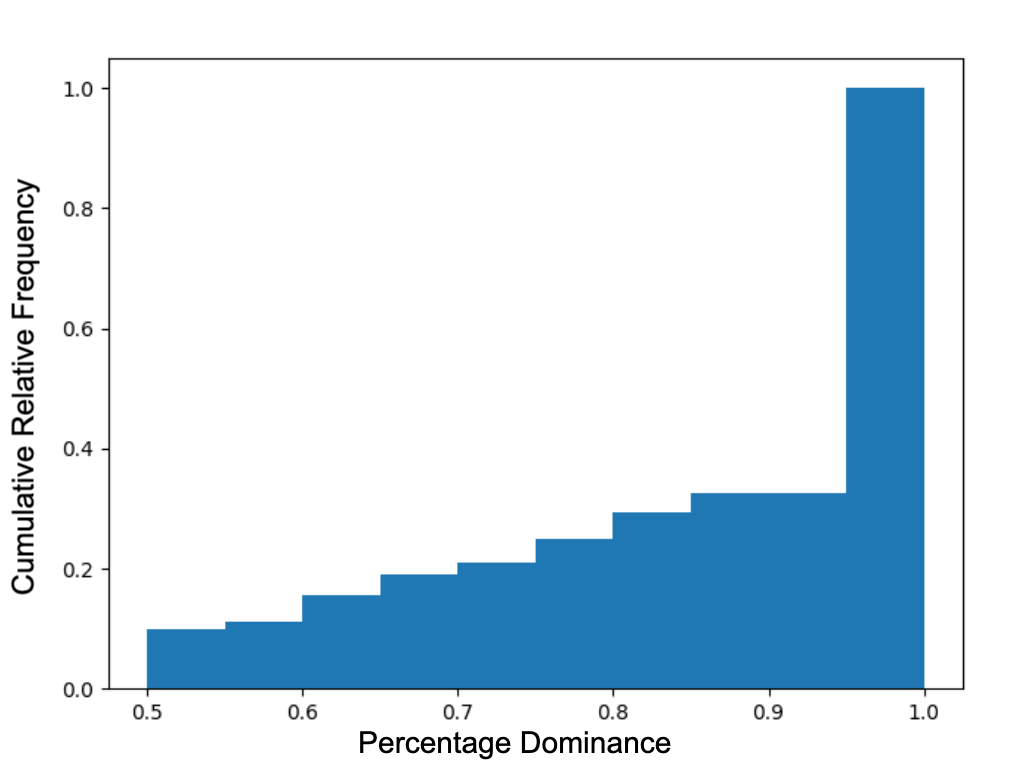
\includegraphics[width=0.5\linewidth]{./assets/experiments/pos_dominance_calculation.png}
  \caption{Cumulative dominance of the most occurring cluster. Dominance of a part of speech tag is measured by the percentage cover that the majority class intakes.}
  \label{fig:POS_dominance}
\end{figure}

It is important to notice that some words did not have enough samples in the SemCor dataset for a significant valuation. 
We intentionally left out classes which had less than $5$ samples.
Also, SemCor is biased, as was previously stated.
However, the results show that quite a majority of the sampled word-classes only contain a single part-of-speech tag, implying that part-of-speech is strongly correlated to meaning.
We continue with a qualitative evaluation of this phenomenon as this is more intuitive to understand.

\subsubsection{Qualitative Evaluation}


To do a qualitative evaluation of this hypothesis, we visualize the BERT vectors using dimensionality reduction techniques.
Due to the disadvantages that each dimensionality reduction techniques carry, we choose to look at $X$ using both PCA and UMAP.
We only look at the polysemous words \Verb#block#, \Verb#run#, \Verb#cold# to keep the analysis concise.

Figures \ref{fig:run_tensorboard} - \ref{fig:cold_tensorboard} show  the tensorboard visualizations.
Please keep in mind that different colors imply different part of speech tags. 
Because the specific value does not play an inportant role, we leave out this legend.

\begin{figure}[H]
\begin{subfigure}{.45\textwidth}
  \centering
  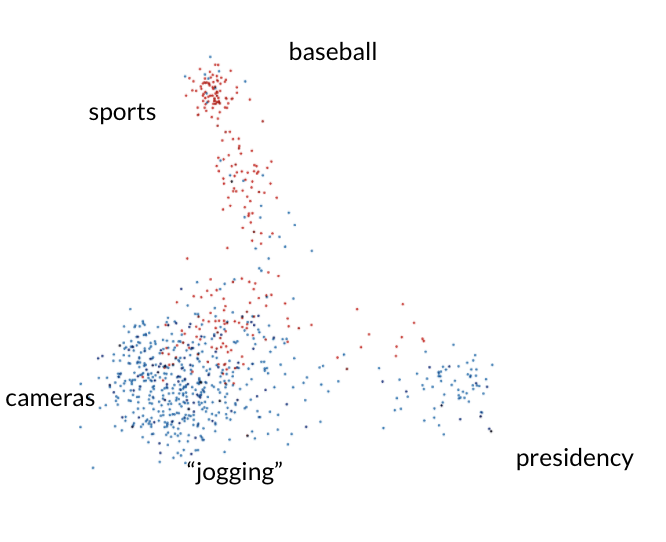
\includegraphics[width=.8\linewidth]{./assets/analysis/run_pca.png}
  \caption{Dimensionality reduction using PCA}
  \label{fig:sfig1}
\end{subfigure}%
\hfill
\begin{subfigure}{.45\textwidth}
  \centering
  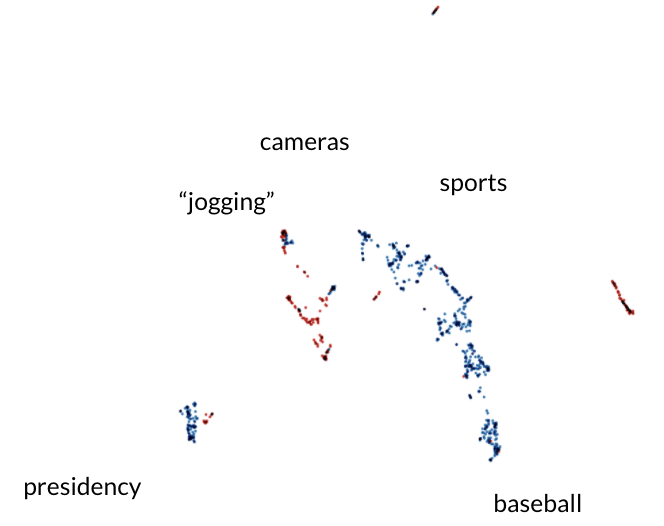
\includegraphics[width=.8\linewidth]{./assets/analysis/run_umap.png}
  \caption{Dimensionality reduction using UMAP}
  \label{fig:sfig2}
\end{subfigure}
\caption{PCA and UMAP visualizations for contextual word embeddings $X$ sampled for the word $w=$\texttt{run}. }
\label{fig:run_tensorboard}
\end{figure}

\begin{figure}[H]
\begin{subfigure}{.45\textwidth}
  \centering
  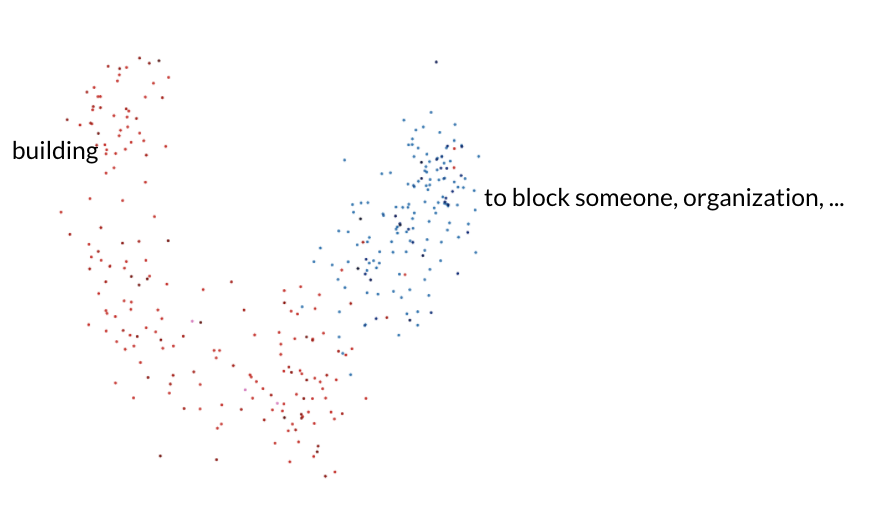
\includegraphics[width=\linewidth]{./assets/analysis/block_pca.png}
  \caption{Dimensionality reduction using PCA}
  \label{fig:sfig1}
\end{subfigure}%
\hfill
\begin{subfigure}{.45\textwidth}
  \centering
  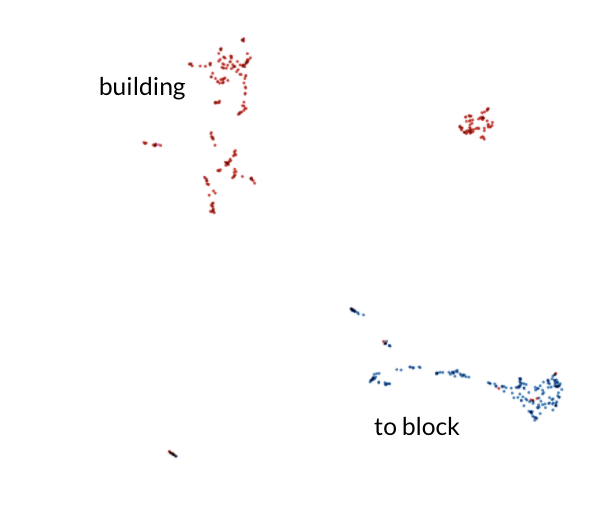
\includegraphics[width=.7\linewidth]{./assets/analysis/block_umap.png}
  \caption{Dimensionality reduction using UMAP}
  \label{fig:sfig2}
\end{subfigure}
\caption{PCA and UMAP visualizations for contextual word embeddings $X$ sampled for the word $w=$\texttt{block}. }
\label{fig:was_tensorboard}
\end{figure}

\begin{figure}[H]
\begin{subfigure}{.45\textwidth}
  \centering
  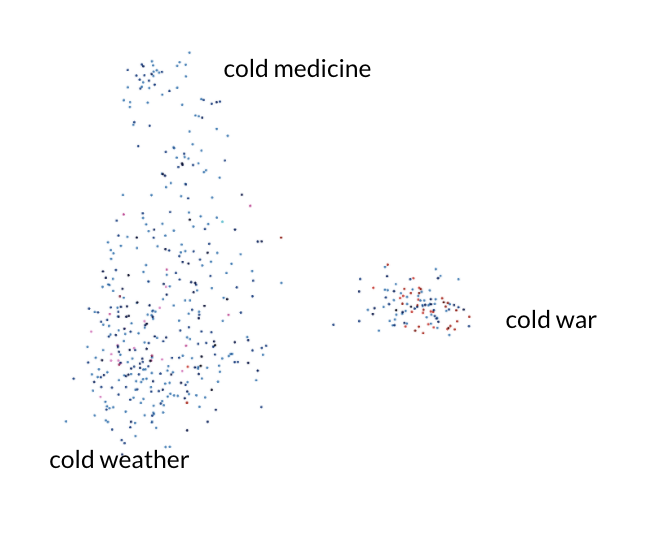
\includegraphics[width=.8\linewidth]{./assets/analysis/cold_pca.png}
  \caption{Dimensionality reduction using PCA}
  \label{fig:sfig1}
\end{subfigure}%
\hfill
\begin{subfigure}{.45\textwidth}
  \centering
  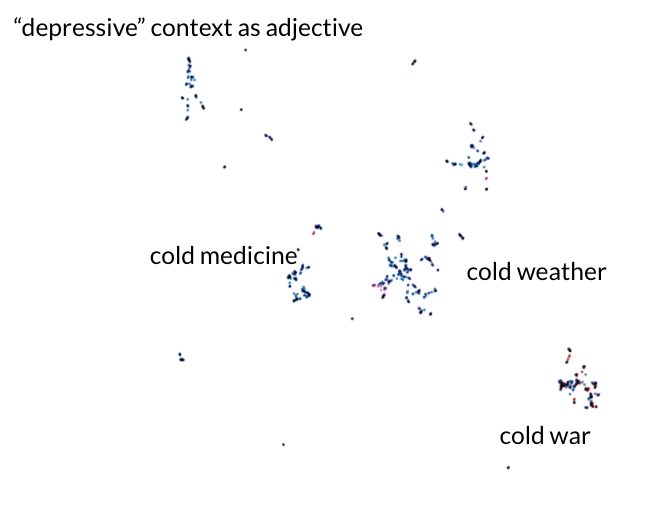
\includegraphics[width=.8\linewidth]{./assets/analysis/cold_umap.png}
  \caption{Dimensionality reduction using UMAP}
  \label{fig:sfig2}
\end{subfigure}
\caption{PCA and UMAP visualizations for contextual word embeddings $X$ sampled for the word $w=$\texttt{cold}. }
\label{fig:cold_tensorboard}
\end{figure}


The following trends are apparent: 
PCA shows a very smooth transition from different semantic classes, whereas UMAP stronlgy shows that clusters are forming between different semantic classes.
This is also true for part-of-speech tags, however, we cannot generalize this as well, because part-of-speech tags strongly correlate with semantics.

Furthermore, one can see that globally BERT does seem to organize the contextual word embeddings by semantics. 
This is apparent in figures \ref{fig:run_tensorboard} and \ref{fig:cold_tensorboard}, where we can see that different blobs (UMAP) and extremes (PCA) in the figures respond to different semantic classes.
Especially in Figure \ref{fig:run_tensorboard} (a), we can see that in the case of UMAP, the central cluster strongly mixes nouns with adjectives (red and blue cluster), and that in the case of PCA, the contextual word embeddings are constrained in such a way that embeddings which mix different semantic classes meet in the middle.
Looking at the different blobs in UMAP we can again confirm the hypothesis that semantics strongly correlates to part-of-speech, as most clusters have a strong predominant color. \\

\chapter{Exploiting subspace organization of semantics of BERT embeddings}\label{section:ExploitingBERT}


So far we have tried to understand how language features are represented within the BERT language model.
Now we want to understand how different modifications to the BERT model affect the performance on language modelling task.
We proceed with GLUE, as it is a very versatile language modelling benchmark.
We will keep the contents of this analysis focused on BERT only, as all transformer models share a similar architecture and as we expect the changes to similarly affect the derivative models.
As such, the focus lies on an ablation study with the BERT model  forming our baseline.
To make the discussion easier, we will refer to any of the models modified by our experiments as \textbf{BERNIE}. 
Please refer to section \ref{section:Background} for a refresher on how sentences are tokenized inside BERT, and how tokens are converted to the latent representation and finally into contextual word embeddings through the BERT model.
\\

Before we continue, we want to introduce the concept of a \textit{split-word}. A split-word is a word for which we will introduce additional embedding vectors in the BERT model, defined by some criterion that depends on the experiment setting.
A split-word will in most cases have high-variance amongst embedding-vectors sampled through BERT.
Introducing more specialized embeddings for tokens with high variance in contextual word embeddings will allow to model more complex distributions.
This happens because we introduce additional weights that can parametrize a specific token distribution, allowing a better approximation of the underlying true distribution.
This would result in multiple simple, well-parametrized probability distributions, rather than a single under-parametrized distribution which has high variance due to the low expressiveness.

\captionof{table}{For each word in the SemCor dataset, the number of WordNet senses, and the mean variance of $n=500$ sampled embedding vectors, across all embedding dimensions. The table shows a subset of the words with highest and lowest variance. There seems to be a strong correlation between the number of WordNet senses and the variance amongst sampled BERT vectors.}
\scalebox{0.9}{
\begin{tabular}{
 l % left aligned column
 l % left aligned column
 c
 c
 c
 %*{3}{S[table-format=4.0]} % three columns with numeric data       
}
\toprule
%TODO MRPC has one aligned, and one unaligned test
\textbf{Word} & \textbf{Number of Senses recorded in WordNet} & \textbf{Mean Variance} \\
\midrule
field & 21  &  0.430 \\
right & 36  &  0.425 \\
forward & 12 & 0.424  \\
general & 10 &  0.422  \\
stands& 24 & 0.393 \\
exchange& 17 & 0.393 \\
\vdots & \vdots & \vdots  \\
loans & 3 & 0.238  \\
rocks & 9 & 0.241  \\
ignore & 5 & 0.275  \\
gasoline & 1 & 0.275 \\
humans & 2 & 0.275 \\
announcement & 2 & 0.275  \\
\bottomrule
\end{tabular}
}

\begin{figure}[H]
	\center
  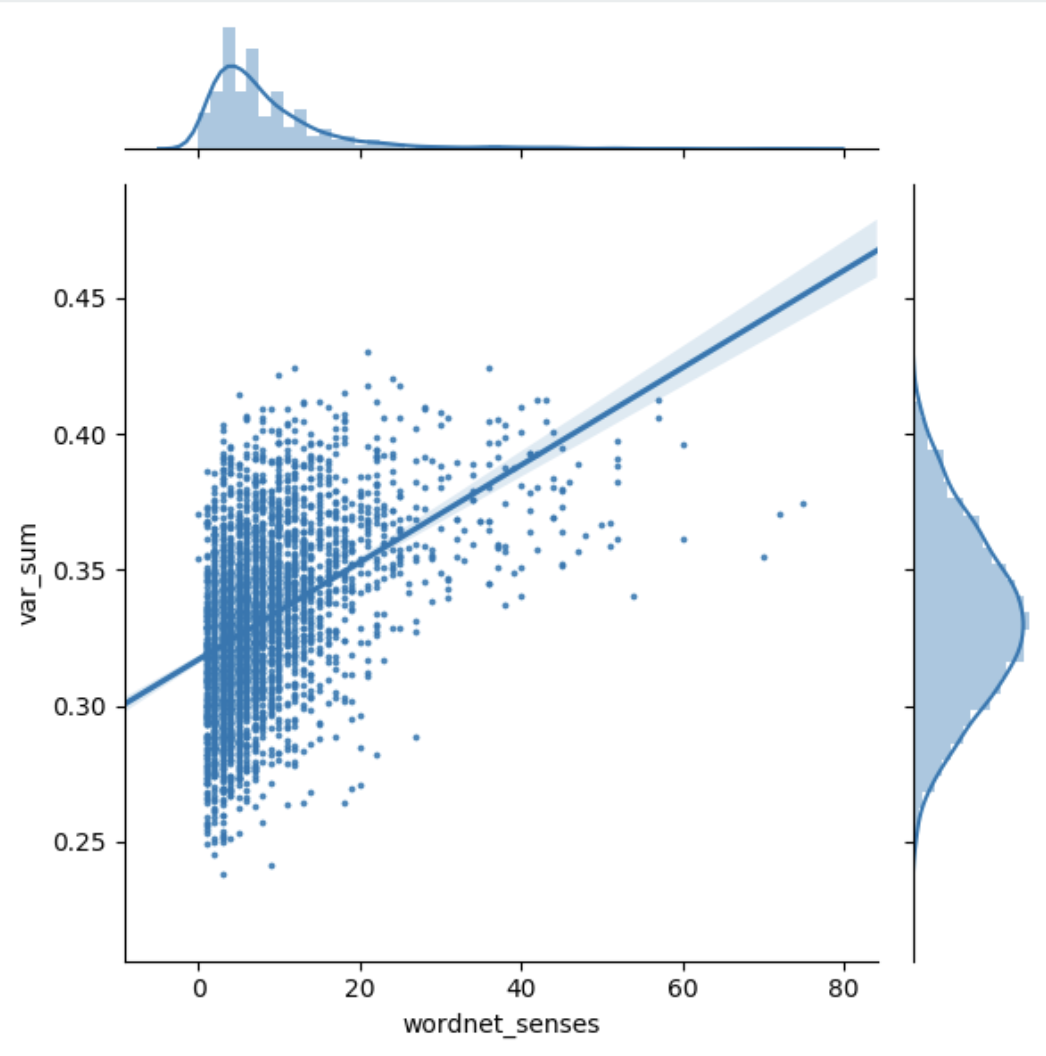
\includegraphics[width=0.5\linewidth]{./assets/experiments/variance_in_BERT_embeddings.png}
  \caption{
  	For each word $w$, we sample both the number of WordNet semantic classes that are recorded in the WordNet dataset. We also calculate the dimension-wise mean variance between $n=500$ sampled vectors for the word $w$. 
  	This constitutes a point on this plot.
  	We repeat this procedure for the most 20'000 most frequent words which consist of a single token (i.e. are not split up into further subtokens when the tokenizer is applied).
	We show that although the variance is relatively high, especially if only few WordNet classes are present, there is a correlation between the number of WordNet classes and the variance of sampled BERT contextual word embeddings.
	The right and top distributions show histograms of how occurrent the variance and WordNet classes are respectively.
	Our assumption is that introducing additional embedding-vectors inside BERT for certain words allows to capture mode complex distributions, i.e. a more complex distribution for words that have a higher number of WordNet classes.
  }
  \label{fig:BERT_variance}
\end{figure}

\section{BERNIE: Equalizing variances across BERT embeddings}

We will introduce two adaptions to the BERT model, BERNIE PoS and BERNIE Cluster.
We will present the results after having introduced both adaptations.
For both modifications, we will use the GLUE dataset to understand what property of the language model is most affected.
In the case of BERNIE Cluster, we use the performance of the downstream task as a proxy to understand what information is captured by the different modes in the data. 
By introducing additional parameters for words with variance (Figure \ref{fig:BERT_variance}), we can see what these embeddings capture the most.
This can be checked by seeing what downstream tasks gain the most performance through the additionally added parameters.

\subsection{BERNIE PoS} \label{bernie_pos}

We want to start with a simple model first.
We have seen in the above section that there is a strong correlation between semantics and part-of-speech.
As such, the initial idea is to introduce additional embedding vectors which are able to capture semantics better.
Because of the strong correlation between the two factors, part-of-speech is used as a proxy for semantics.
One of the advantages that this carries is that we can use the spaCy part-of-speech tagger \cite{spacyb} to classify the part-of-speech tags with high accuracy.

Our first model adoption is called \textbf{BERNIE PoS}.
In this case, we introduce new tokens, and new embedding vectors into the embedding layers of the transformers inside of BERT.

\subsubsection{Experiment setup}

BERNIE PoS introduces one new embedding vector for each possible part-of-speech configuration of the split-words.
As an example, instead of having a single embedding vector for the word \Verb#run#, we introduce two new embeddings \Verb#run_VERB# and \Verb#run_NOUN#, which both replace the intial \textit{run}-embedding. 
We will refer to \Verb#run_VERB# and \Verb#run_NOUN# as so called \textit{sub-embeddings}, as these exploit the subspace structure of the contextual word embeddings sampled for the word \Verb#run#.
As for the tokenizer, we also introduce a mechanism which turns any occurrence of \Verb#run# into one of the sub-embeddings.
Specifically, our part-of-speech modified pipeline is presented in Figure \ref{fig:BERnie_POS_pipeline}.

\begin{figure}
	\center
  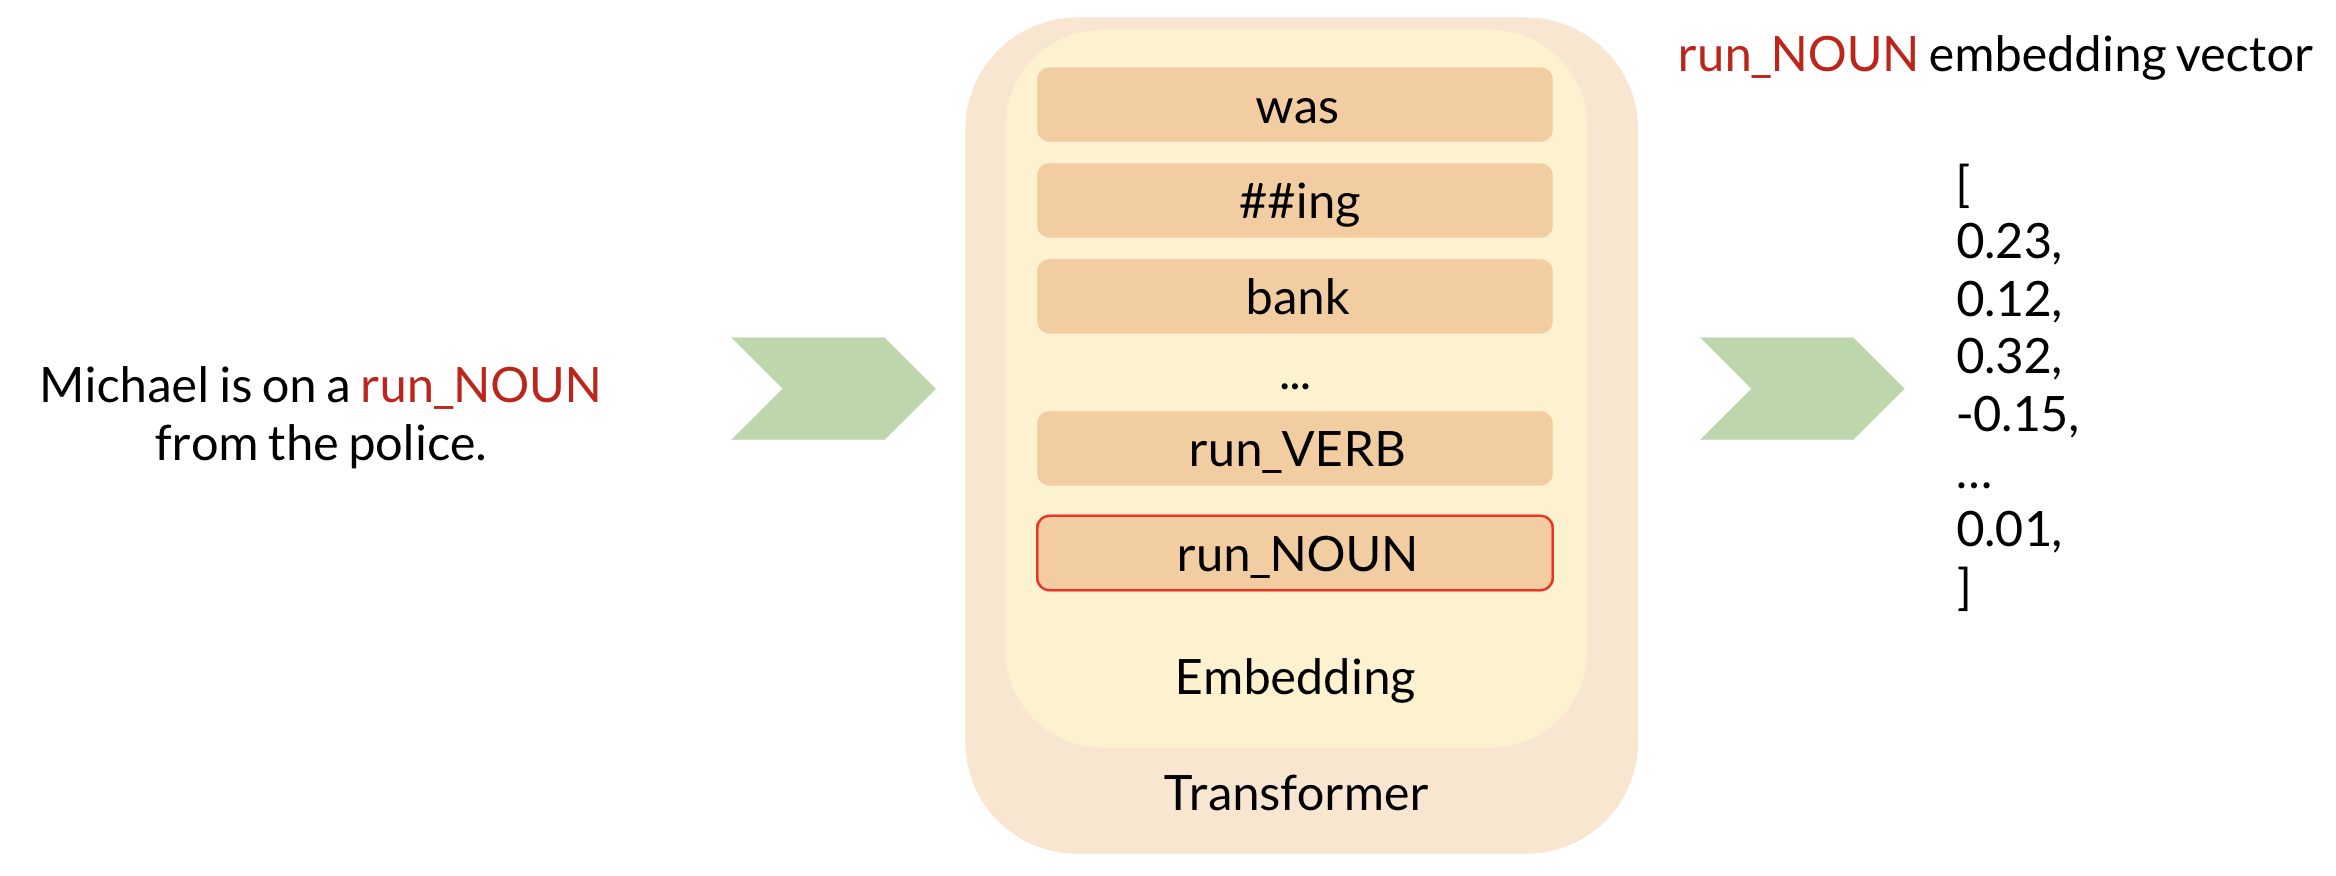
\includegraphics[width=\linewidth]{./assets/experiments/pipeline_tokenizer_BERnie_POS_input.png}
  \caption{The part-of-speech modified pipeline. 
  The BERNIE PoS model takes as input a sentence $s$. The sentence $s$ is converted to a sequence of BERT tokens $[t_1$, \ldots, $t_m]$ as defined in a given vocabulary $V$.
    This vocabulary $V$ is extended with the additional tokens for each of the split-words.
For each target token $t_{\text{target}}$, we make the token more specific by converting the token to a more specialized token-representation, which specifies the part-of-speech information as part of the token.
In this case, $run$ becomes the more specialized $run\_ VERB$.
Again, each item in the vocabulary $V$ has a corresponding embedding vector inside the embedding layer of the transformer.
}
  \label{fig:BERnie_POS_pipeline}
\end{figure}

%TODO space

To identify whether the occurring \Verb#run# in an example sentence is a verb or a noun, we use the spaCy part-of-speech tagger \cite{spacyb}, which claims 92.6 \% accuracy for this task.
When initializing the embeddings for the newly introduced embeddings, we copy the weights of the original embedding.
This is depicted in Figure \ref{fig:BERnie_POS_initialization}.
The final pipeline is presented in \ref{fig:BERNIE_POS_full_pipeline}.
During training, all weights of BERT are fine-tuned to the downstream GLUE task as described in section \ref{section:Background}.

\begin{figure}
	\center
  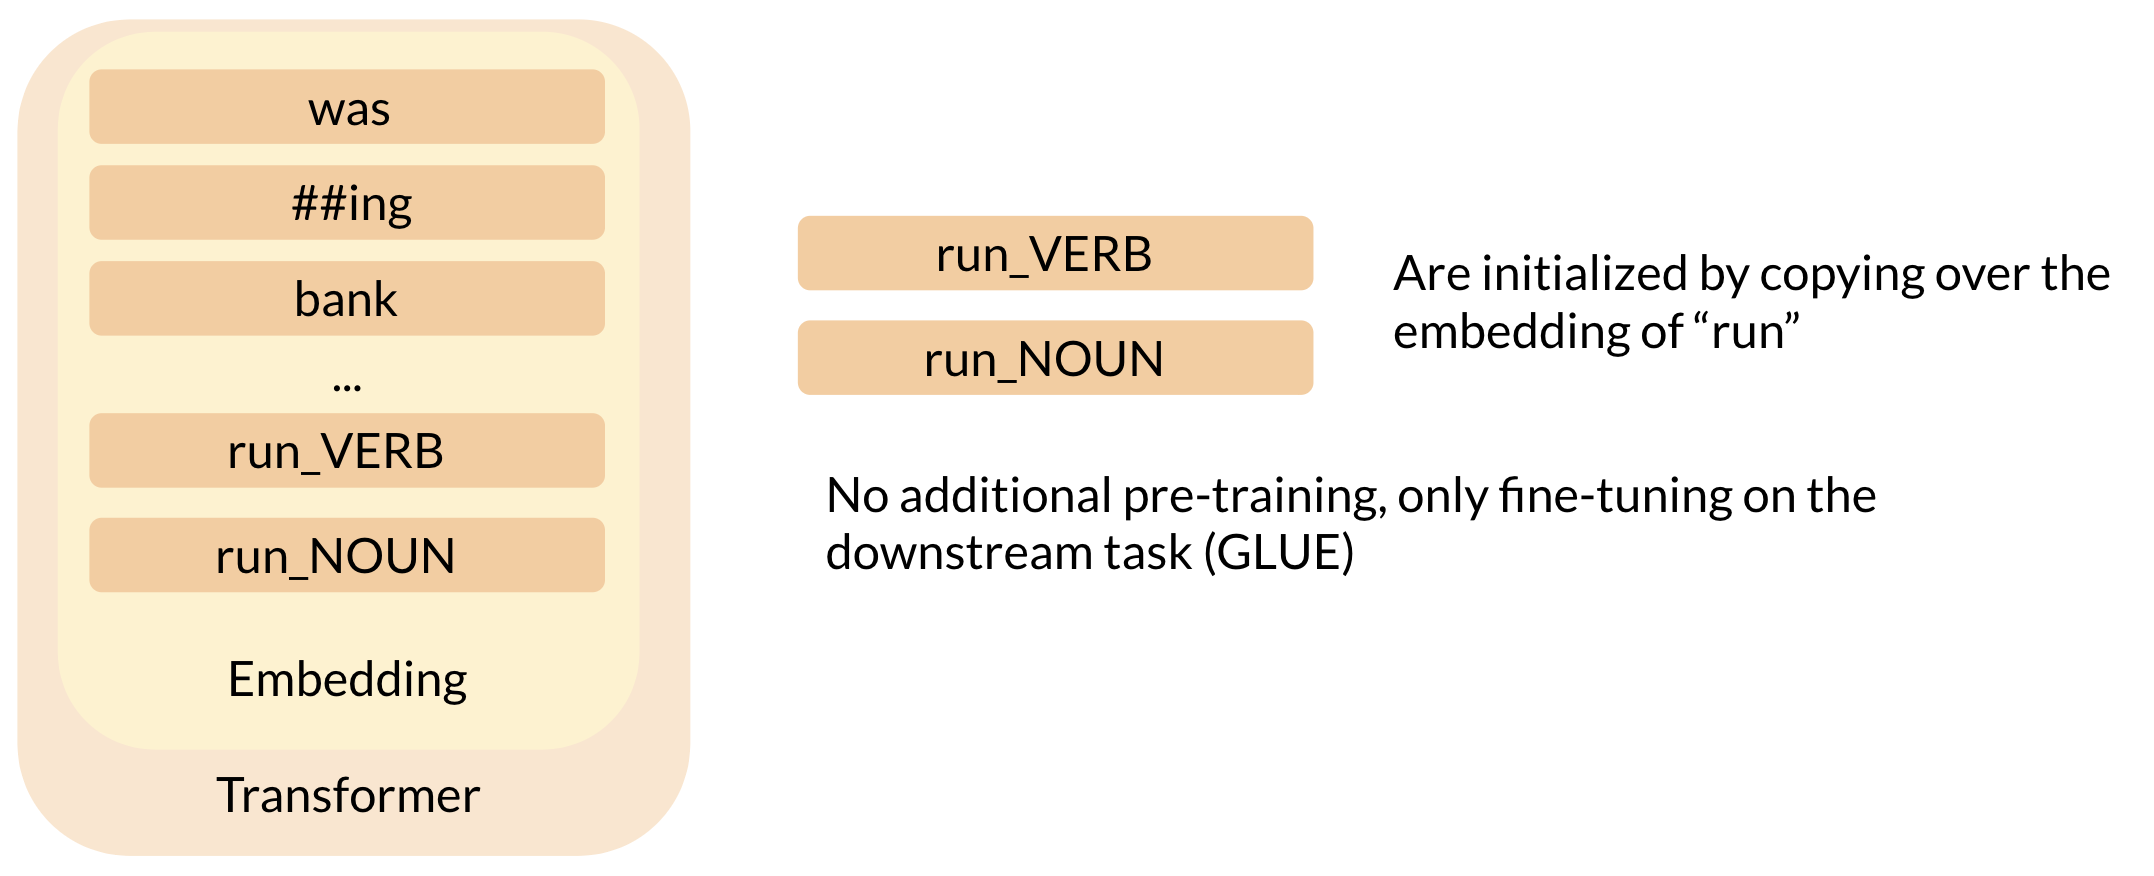
\includegraphics[width=\linewidth]{./assets/experiments/pipeline_model_BERnie_POS_initialization.png}
  \caption{Inside the embedding layer of the transformer which occurs at each layer of BERT, we introduce more specific embeddings \texttt{run\_VERB} and \texttt{run\_NOUN}. The BERT model should now capture more expressiveness, as more weight got introduced for a part of the model which results in a probability distribution with high variance. The original \texttt{run} embedding is removed.}.
  \label{fig:BERnie_POS_initialization}
\end{figure}

\begin{figure}
\begin{subfigure}{.52\textwidth}
  \centering
  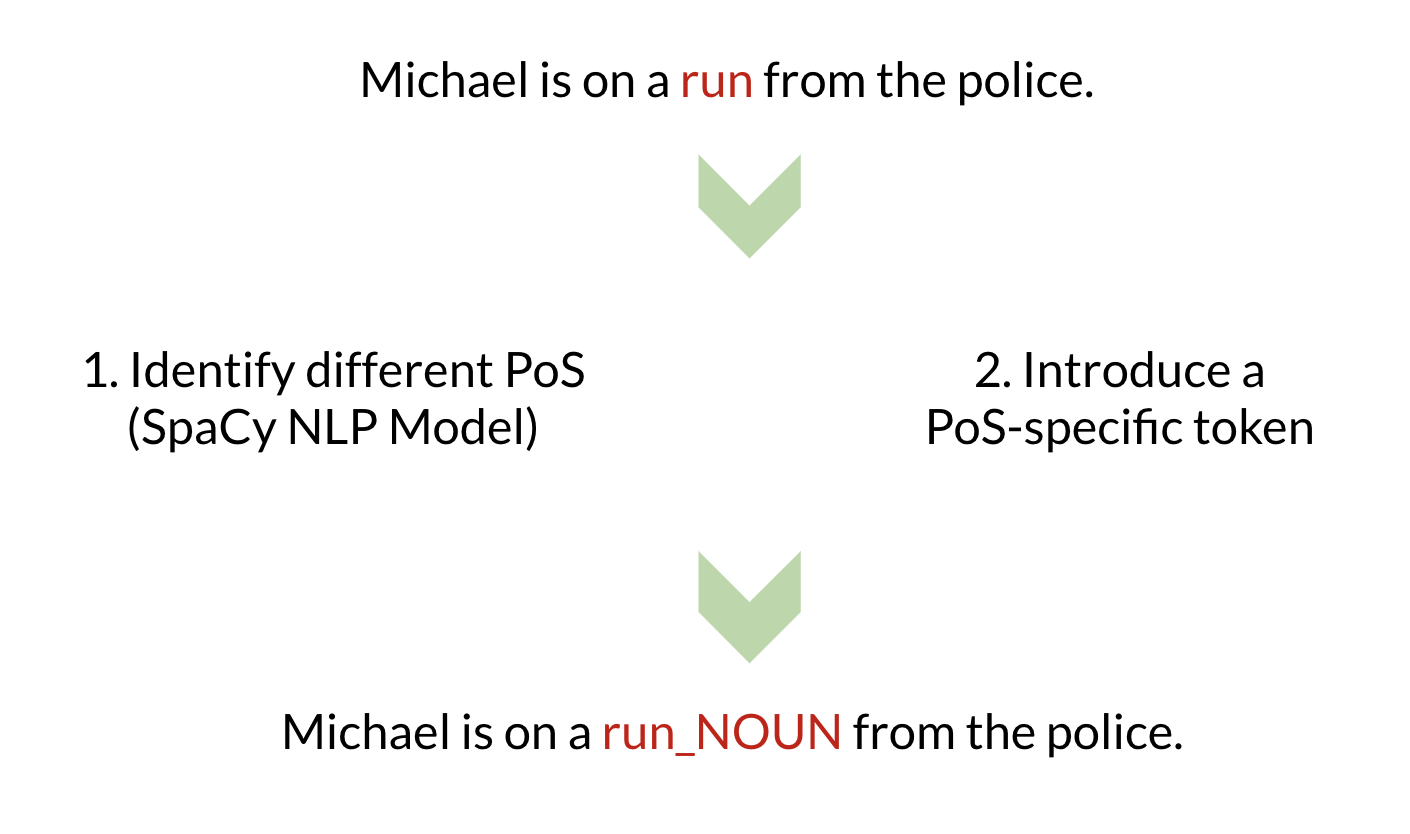
\includegraphics[width=\linewidth]{./assets/experiments/pipeline_tokenizer_BERnie_POS_sentence.png}
  \caption{The part-of-speech modified tokenizer pipeline.}
  \label{fig:sfig1}
\end{subfigure}%
\hfill
\begin{subfigure}{.54\textwidth}
  \centering
  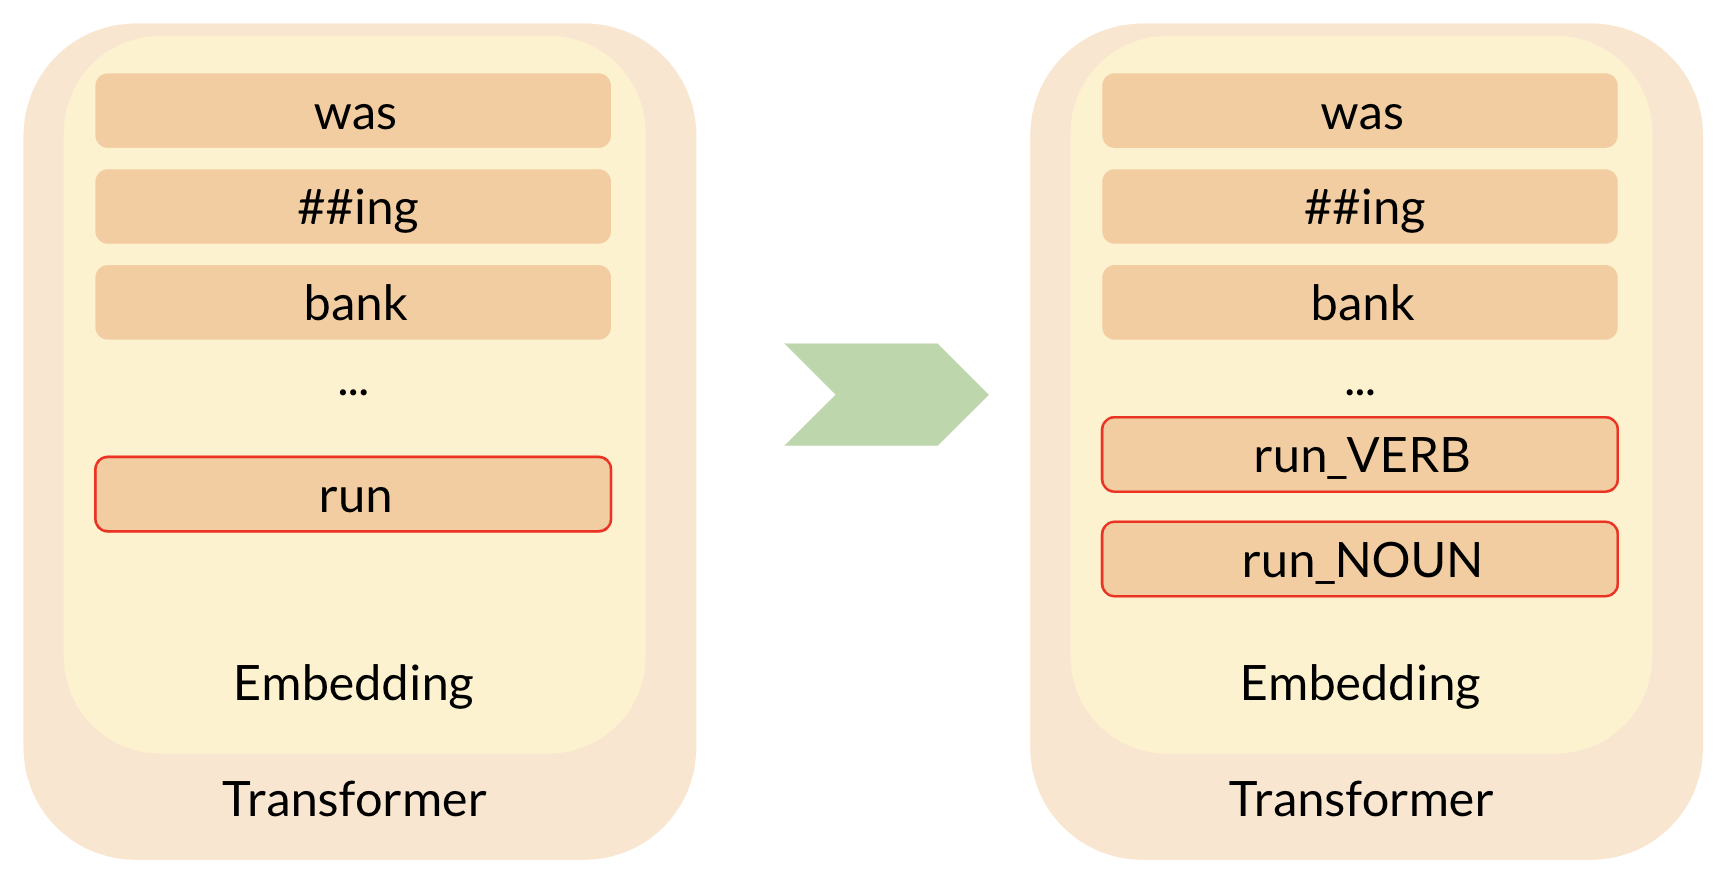
\includegraphics[width=\linewidth]{./assets/experiments/pipeline_model_BERnie_POS.png}
  \caption{The PoS modified BERT embedding.}
  \label{fig:sfig2}
\end{subfigure}
\caption{The resulting, fully modified BERNIE PoS pipeline.}
\label{fig:BERNIE_POS_full_pipeline}
\end{figure}

\subsection{BERNIE Cluster}\label{experiment_bernie_meaning}

BERNIE Cluster introduces new tokens and their respective embeddings in the transformer embedding layer, similar to the previous section \ref{bernie_pos}.
This time however, we do not introduce new tokens by part-of-speech, as we did in the previous section, but rather by the clustering algorithms above.
Although the hyperparameter optimization method optimized for the best overlap with coarseness of semantic classes as defined by WordNet, it is not quite interpretable to what these different clusters correspond to (as discussed in section  \ref{experiment_BERT_clusterability}).
This is partially also because we cannot formally capture the concept of semantics or part-of-speech.
In section \ref{experiment_BERT_clusterability}) we had seen that these clusters do not correspond to WordNet semantic classes in general, however we could also apply a per-case analysis of this.
The aim of this experiment-model is to find out what these clusters correspond to the most, and we will use the GLUE benchmarks to understand what tasks this clustering-information benefits or detriments the most.
This should give us a more generalizable idea of how the added parameters - dependant on the clustering assignments - affect downstream tasks.
For convenience in explaining, we will make use of intuitive concepts like \texttt{bank\_ FINANCE} and \texttt{bank\_ SEA} for convenience, and because this is our core assumption that we aim to disprove.
We will mention whenever this assumption does not seem to hold.

\subsubsection{Experiment setup}

Again, our base model is the standard BERT model from section \ref{section:BERT} .
We now also modify the tokenizer in such a way, that split-words are replaced with a more specific token.
As an example, we want to replace the word $bank$ with a token, which captures whether or not the $bank$ that we refer to implies a 1) financial institution, or 2) a river bank.
We use the clustering approach introduced in Section \ref{experiment_BERT_clusterability} as the intermediate model to distinguish on which semantic class the sentence refers to.
We also introduce new embedding vectors that the new tokens correspond to.
However, please keep in mind that these clusters generally do not seem to refer to semantic classes (section \ref{experiment_BERT_clusterability}), but we will use this as our assumption until we find data to contradict this.
After we have concluded these changes, we arrive at the following model, which has a modified tokenizer, and a modified BERT model.
We call the corresponding model \textbf{BERNIE Cluster}.

\begin{figure}
	\center
  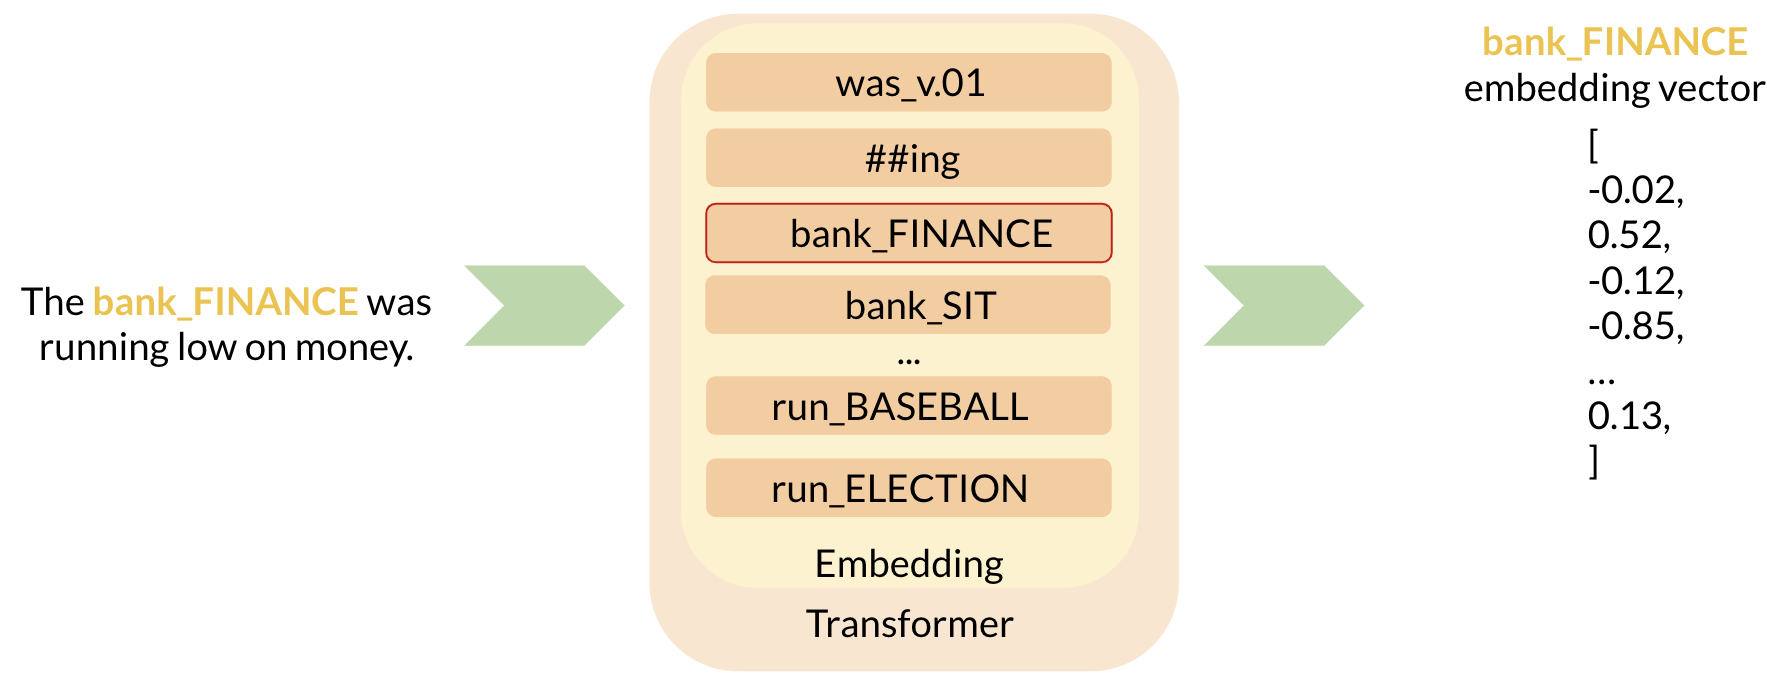
\includegraphics[width=\linewidth]{./assets/experiments/pipeline_model_BERnie_meaning.png}
  \caption{The semantic modified pipeline. 
  The BERNIE Cluster model takes as input a sentence $s$. The sentence $s$ is converted to a sequence of BERT tokens $[t_1$, \ldots, $t_m]$ as defined in a given vocabulary $V$.
  This vocabulary $V$ is extended with the additionally introduced tokens for each of the split-words.
For each target token $t_{\text{target}}$, we make the token more specific by converting the token to a more specialized token-representation, which specifies the clustereing information as part of the token.
In this case, $bank$ becomes the more specialized $bank\_FINANCE$.
Again, each item in the vocabulary $V$ has a corresponding embedding vector inside the embedding layer of the transformer.
This embedding vector is used by the intermediate layers of the transformer, and thus affects the downstream pipeline of the language model for any subsequent layers of the transformer.}
  \label{fig:BERT_Cluster_pipeline}
\end{figure}


\begin{figure}
\center
\begin{subfigure}{.54\textwidth}
  \centering
  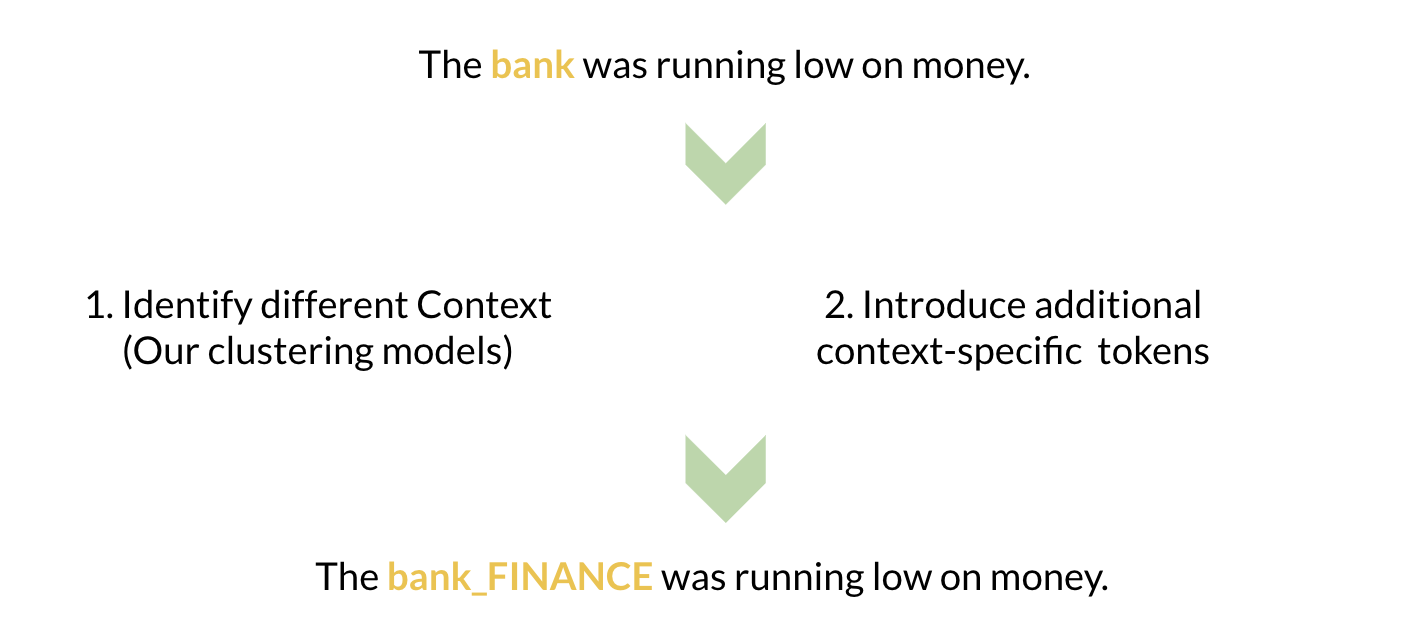
\includegraphics[width=\linewidth]{./assets/experiments/pipeline_tokenizer_BERnie_meaning.png}
  \caption{The clustering-modified tokenizer pipeline}
  \label{fig:sfig1}
\end{subfigure}%
\begin{subfigure}{.5\textwidth}
  \centering
  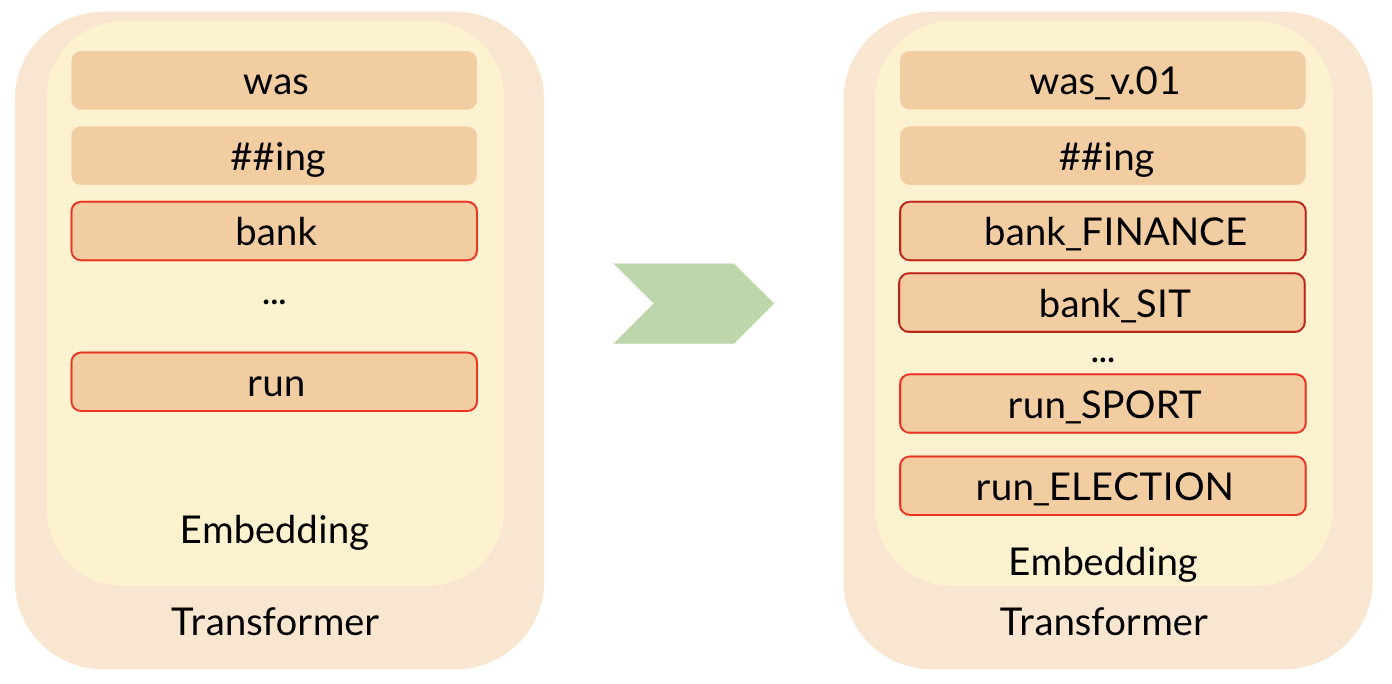
\includegraphics[width=\linewidth]{./assets/experiments/pipeline_model_BERnie_meaning_embedding.png}
  \caption{The clustering-modified BERT embedding}
  \label{fig:sfig2}
\end{subfigure}
\caption{The resulting, fully modified BERNIE Cluster pipeline.}
\label{fig:fig}
\end{figure}


\subsubsection{Results}

We now do an evaluation of the introduced BERNIE PoS and BERNIE Cluster model.
Weights which are instantiated specifically for the GLUE tasks (final layer) are once instantiated with a random seed of 42, and once with a random seed of 101.
The scores are the mean of the two runs.

\begin{table}[H]
\center
\scalebox{0.9}{
\begin{tabular}{
 l % left aligned column
 l % left aligned column
 c
 c
 c
 c
 c
 % *{5}{S[table-format=4.0]} % three columns with numeric data       
}
\toprule
\textbf{Task} & \textbf{Score Measure} &\textbf{BERT} & \textbf{BERNIE PoS} & \textbf{BERNIE Cluster} \\
\midrule
CoLA  & Accuracy  &  \textbf{0.5739} & 0.5263 &  0.5457 \\

MRPC & Accuracy &  \textbf{0.8223} & 0.8199 &  0.8064 \\
          & F1           &  \textbf{0.8778} & 0.8614  &  0.8684 \\
          & Mixed     &  0.8501 & \textbf{0.8579}  &  0.8374 \\
          
SST-2 & Accuracy  &  0.9214 & 0.9203 &  \textbf{0.9266} \\

STS-B & Correlation &  \textbf{0.8841} & 0.8615 &  0.8574 \\
      & Pearson & \textbf{0.8860} & 0.8621         & 0.8587 \\
      & Spearman & \textbf{0.8822} & 0.8601      & 0.8567 \\
      
QNLI & Accuracy &  \textbf{0.9126} & 0.9090    &  0.9020 \\

RTE & Accuracy &  \textbf{0.6462} & 0.6083     &  \textit{0.5722} \\

WNLI & Accuracy &  \textit{0.35915} & 0.3947 &  \textbf{0.4649} \\

MNLI & Accuracy &  0.8453 &              &  0.8334 \\

SNLI & Accuracy &  \textbf{0.8461} &              &  0.8367 \\

QQP & Accuracy &  \textbf{0.9113} &              &  0.9042 \\
      & F1     & \textbf{0.8809} &                       & 0.8732 \\
      & Mixed & \textbf{0.8961} &                    & 0.8887 \\
      
\bottomrule

\end{tabular}
}
\caption{GLUE Benchmark performance measures for the BERT model, BERNIE PoS and BERNIE Cluster.
Higher scores are better.
The task-wide best-performers are marked in bold.
All values are the average scores of two runs.
}
\end{table}


One can see that for most tasks, the BERNIE model modifications has negative effect on most GLUE tasks.
We assume that this is either because the newly initialized embeddings were not pre-trained like the other embeddings (on a 3.3 billion word sized corpus), and also because the part-of-speech (accuracy of 92.6\%) and clustering (accuracy less than 100\%) models propagate an error term to the embedding-lookup task.
On the other side, the WNLI and RTE experiments are considerably deviating in performance through the addition of the the sub-embeddings.
Both are often considered the most difficult GLUE tasks.
For the BERNIE Cluster model, WNLI performs better (\textbf{10.56\%}) than standard BERT, and RTE performs worse  (\textbf{-7.40\%}) than the standard BERT implementation.
Similar results are observable for the difference between the unmodified BERT and the BERNIE PoS model with \textbf{3.52\%} improvement for WLNI and \textbf{-3.79\%} decline in performance for the RTE task.

WNLI and RTE are both natural language induction tasks \ref{section:Background}.
RTE focuses on a textual entailment task. 
It does not seem far off that performance here drops further, as most of the datasamples do not test for word disambiguatiy, but rather for the ability to capture the "global" idea of the sentence.
Thus, we assume that the newly added embeddings are not mature enough to distinctively capture the different concepts, but that too much noise was added (through the embedding-lookup mechanism, and the newly added embeddings), that performance deteriorates.
In contrast, the WNLI task improves in task performance where the focus is on target words. 
Specifically WNLI does not only look at the global idea captured by the sentence (as is done with RTE), but looking at individual words to understand what is the pronoun for a referent.
It seems apparent that making the word-sense more explicit by introducing specialized tokens and embeddings can help cut ties with this task.
Because WNLI has a low performance, it could also be that the added weights capture other latent information within the embeddings, showing that the embedding projection is a bottleneck of the BERT model for tasks similar to WNLI.
Also, compared to BERNIE PoS, the BERNIE Cluster model amplifies the performance-difference to BERT in both the negative and positive direction.
We assume that this is because BERNIE Cluster implements a clustering module, which is able to partition the BERT space much more smoothly than the part-of-speech tagger does.

\subsection{BERNIE Cluster with additional pre-training}

One of the trends we see is the overall negative trend in performance.
This might be due to the newly initialized vectors not being calibrated enough, i.e. not pre-trained on a large-enough corpus (as is done with the rest of the embedding vectors \cite{devlin18}), but only fine-tuned for GLUE tasks on limited data.
Thus we measure the performance of BERNIE models after additional pre-training.

\subsection{Experiment setup}

We want to test to what extent pre-training the newly initialized embeddings helps improve the performance on the embeddings.
We apply 1 epoch of pre-training on the news corpus described in Section 2.
We instantiate the additional embeddings as described in the previous section.
We then run one full epoch of training with the same training parameters as used for GLUE on the \textbf{news.corpus.2007} dataset using a masked language model methodology as described in section \ref{section:Background}.
We save this model and load it for the GLUE tasks.
BERNIE full Pre-training trains all the embeddings, whereas BERNIE partial Pre-Training fixates all embedding vectors except the ones that were newly added.
\textbf{BERNIE full Pre} allows the gradients to update all the embedding weights during pre-training.
\textbf{BERNIE partial Pre} only allows gradient updates for the embeddings of the newly added vocabulary items, i.e. the split-words.
Specifically, only the newly added embeddings vectors are calibrated, while all other embedding vectors are kept constant.

\subsection{Results}

Again, we run the experiments and show the results as the average of two runs.
Due to time-constraints and certainty of bugs for some experiments, we only show the results for a subset of the GLUE tasks.

\hfill \break

\scalebox{0.9}{
\begin{tabular}{
 l % left aligned column
 l % left aligned column
 c
 c
 c
 %*{3}{S[table-format=4.0]} % three columns with numeric data       
}
\toprule
%TODO MRPC has one aligned, and one unaligned test
\textbf{Task} & \textbf{Score Measure} & \textbf{BERNIE} & \textbf{BERNIE full\- Pre}  & \textbf{BERNIE partial\- Pre}\\
\midrule
CoLA  & Accuracy  &  0.5457 & 0.5418 & \textbf{0.5731} \\
SST-2 & Accuracy  &  \textbf{0.9266} & 0.9169 & \textbf{0.9266} \\
QNLI & Accuracy & \textbf{0.9020} & 0.5374 & 0.6700 \\
RTE & Accuracy &  \textbf{0.5722} & 0.4784 & 0.4729 \\
WNLI & Accuracy & \textbf{0.4649} & 0.4225 & 0.4507 \\
\bottomrule
\end{tabular}
}
\captionof{table}{GLUE Benchmark performance measures for the BERNIE Cluster model without any additional pre-training, the BERNIE Cluster with full pre-training and BERNIE with partial pre-training.
Higher scores are better.
The task-wide best-performers are marked in bold.
All values are the average scores of two runs.}

\hfill \break

As one can see, the additional pre-training does not improve performance on most of the GLUE tasks.
However, we assume that this is due to the pre-training corpus not being similar to the pre-training corpus that was initially used for BERT (which is too big to be run for this test), or the hyperparamters not being optimal for this run.
Finally, it could also be that the initialization for the newly added vectors was suboptimal, as we have seen strong deviations (of up to 5\% in performance) over different random seeds for the GLUE tasks.
Due to time-constraints, we decided to not move ahead with this experiment.

\chapter{Conclusion}\label{section:Conclusion}

We focuses our analysis on how contextual word embeddings produced by BERT capture \textit{semantics}. 
We analyse the outputs of the BERT language model, as it provides a good balance between popularity, close to state-of-the-art performance, and generalizability to other modern language models.

\section{Main Contributions}

Our main observations are the following: \\

\begin{enumerate}
\item We test for linear separability and ability to partition the space into semantic clusters within the sampled BERT vectors.
We show that while linear separability is possible, it is nearly impossible to find modes in the data which correspond to semantic classes that are as distinctively as defined by WordNet.
We conclude that BERT organized the embedding vectors imminently by context, and not by semantics alone.
This can easily introduce undesirable properties such as strong sentiment as observed in one of our experiments, leading to considerable bias in downstream tasks.
\item We analyze the relationship between the two linguistic features of part-of-speech and semantics. 
We show that these show a strong correlation in languages and that modern language models capture this strong correlation.
This affects the conclusion of some related work which had analysed language models which capture semantics, but which did not account for the correlation between part-of-speech and semantics.
\item Finally, we introduce additional parameters for words whose sampled embedding vectors have high variance over the embedding space.
We investigate what downstream tasks are most affected by these changes and use this as a proxy to understand what the clustering assignments correspond to. 
\end{enumerate}

\hfill \break

Our findings show that BERT does not capture an easily interpretable semantic subspace, it rather imminently organizes the embeddings purely by context.
This can often introduce undesirable features such as strong sentiment, position in sentence, and thus lead to considerable bias in downstream applications.

\section{Future Work}

Because we were only able to investigate some of our core hypotheses, different directions for future work are imminent.
These could include or investigate:

\paragraph{Introducing the WiC benchmark:} One of our main targets with the modifications made by BERNIE Cluster was to analyse what effect this modification has on semantics, specifically polysemy.
An ablation study on other benchmarking datasets, most specifically the Word in Context benchmark which is included in SuperGLUE would have been a valuable addition to understand what our modifications have to the modelling power of language models.

\paragraph{Larger benchmarking dataset:} Within our analysis, we have had numerous occasions where the statistical significance and testing power largely suffered due to the limited size of gold-standard datasets which capture semantics.
SemCor is one of the most extensive dataset available in this domain, but is still too small to do proper evaluation on.
This limits the choice of polysemous words analysed in Section \textbf{(4)}.
A bigger labelled dataset would lead to a more expressive analysis.

\paragraph{Semantic subspace not apparent:} An interesting line of future work could lie in analysing whether a semantic is only apparently locally (per word $w$), or whether a global principal component capturing semantics exists.
Latter could be done using distance metric learning (see Appendix \ref{appendix:metric_learning}).

\paragraph{Formalizing semantics:}
Intuitively, we have often seen that certain words such as \texttt{was} were overdefined in terms of semantic classes, where many dozen semantic classes are apparent.
Generally, it is difficult to quantify "coarseness" between semantic concepts, apparent in section \textbf{(4)}.
A more quantified definition would be beneficial in defining semantics.

\paragraph{Limited coherence in lines of work} 
Different authors seem to analyse this topic using different tools, leading to partially incoherent statements.
Also, the nature that linguistic features are strongly correlated (i.e. part-of-speech and semantics), is not properly noted by a lot of previous work, making conclusions on semantics when part-of-speech was analysed.
Establishing a more formal framework could address this, and the previously mentioned issue.

\appendix
\singlespacing

% \bibliographystyle{unsrt} 
%TODO change bibliography style
\bibliographystyle{plain}
% \bibliographystyle{apa-good}
% \bibliographystyle{mla-good}
\bibliography{dissertation} 

\chapter{Background}

\section{Linguistic features}\label{appendix:linguistic_features}

\paragraph{Other linguistic features} are recorded in \cite{wang19} and include

\begin{table}[h!]
\centering
\begin{tabular}{l l} 
 \hline
 Coarse-Grained Categories & Fine-Grained Categories \\ [0.5ex] 
 \hline
 Lexical Semantics & Lexical Entailment, Morphological Negation, Factivity, \\
&  Symmetry/Collectivity, Redundancy, Named Entities, \\
& Quantifiers \\ 
Predicate Argument Structure & Core Arguments, Prepositional \\ & Phrases, Ellipsis \/ Implicits, \\
& Anaphora/Coreference Active/Passive, Nominalization, \\
& Genitives/Partitives, Datives, Relative Clauses, \\
& Coordination Scope, Intersectivity, Restrictivity \\
Logic & Negation, Double Negation, Intervals/Numbers, \\
& Conjunction, Disjunction, Conditionals, Universal, \\
& Existential Temporal, Upward Monotone \\
& Downward Monotone, Non-Monotone \\
Knowledge & Common Sense, World Knowledge \\ [1ex] 
\hline
\end{tabular}
\caption{Table from \cite{wang19}. Types of linguistic phenomena organized under four major categories.}
\label{table:1}
\end{table}

\section{Gaussian Embeddings}\label{appendix:GaussianEmbeddings}

\cite{bengio06} already used distributional representations to embed concepts from natural language processing into embeddings.
\cite{vilnis14} considers creating a Gaussian representation for each word token, resulting in Gaussian static word embeddings.
This can be interpreted as a probabilistic and continuous extension to the discrete point vectors calculated by word2vec and GloVe.
Each word is represented by a Gaussian distribution in high-dimensional space, with the aim to better capture uncertainty when doing algebraic operations on the word-embeddings, resulting in a model which expresses the relation between words and their representations better.
Using KL-divergence as a distance metric, it can also express asymmetric relations more naturally than dot-products or cosine similarities do.  
Specifically, the newly emerging embedding for word $w$ can be modelled by the tuple 

$$
\theta_w = ( \mu_w,  \Sigma_w)
$$

and the probability density function of the static word embedding $x_w$ is expressed by

\begin{equation}
p(x; w) = \mathcal{N}\left(x ; \mu_{w}, \Sigma_{w}\right)
\end{equation}

where $x$ is a point in the embedding space. \\

Given that the probability density function is given by a gaussian distribution, the loss functions which is minimized is adapted accordingly:

\begin{equation}
L_m(w, c_p, c_n) = - min(0, m - E_\theta(w, c_p) + E_\theta(w, c_n) )
\end{equation}

where $E$ is the energy function which calculates the distance measure between word $w$, a positive context word $c_p$ (a word that co-occurs with the word $w$, and $c_n$), and a negative-sampled context word $c_n$ (a word that does not co-occur with the word $w$, usually randomly sampled from the set of all words in the vocabulary $\mathcal{V}$).
\cite{vilnis14} proposes two different ways to compute the energy function, using a symmetric similarity, and an asymmetric similarity measure. \\

The energy function can be \textbf{symmetric}.
In this case, the authors use an inner product of two gaussian distributions defined as:

\begin{align}
E_\theta(w, c) &= \int_{x \in \mathcal{R}^d} f(x)g(x) dx \\
&= \int_{x \in \mathcal{R}^d} \mathcal{N}(x; \mu_w, \Sigma_w) \mathcal{N}(x; \mu_c, \Sigma_c) dx \\
&= \mathcal{N}(0; \mu_w - \mu_c, \Sigma_w + \Sigma_c)
\end{align}

which results in a nice closed form representation. 

The energy function can also be \textbf{asymmetric}.
In this case, the authors refer to the KL-divergence, resulting in the following energy function minimized.

\begin{align}
-E(w_i, c_j) & = D_{KL}(c_j || w_i) \\
&= \int_{x \in \mathcal{R}^d} \mathcal{N}(x; \mu_{w_i}, \Sigma_{w_i}) \text{log} \frac{\mathcal{N}(x; \mu_{c_j}, \Sigma_{c_j})}{\mathcal{N}(x; \mu_{w_i}, \Sigma_{w_i})} dx \\
&= \frac{1}{2}\left(\operatorname{tr}\left(\Sigma_{i}^{-1} \Sigma_{j}\right)+\left(\mu_{i}-\mu_{j}\right)^{\top} \Sigma_{i}^{-1}\left(\mu_{i}-\mu_{j}\right)-d-\log \frac{\operatorname{det}\left(\Sigma_{j}\right)}{\operatorname{det}\left(\Sigma_{i}\right)}\right)
\end{align}

The asymmetric distance property allows to capture relations such as "y entails x", without necessarily implying "x entails y".

Assuming training was conducted by one of the two presented models,  one can use the resulting model parameters for two words $x_{w_1}, x_{w_2}$ to calculate the uncertainty - which intuitively models the similarity between the two words $w_1$ and $w_2$.
This is analogous to calculating the dot product between the two distributions $P(z=x^T y)$ through the close-form formulation of

\begin{align}
\mu_z &= \mu_x^T \mu_y \\
\Sigma_z &= \mu_{x}^T \Sigma_{x} \mu_{x}+\mu_{y}^T \Sigma_{y} \mu_{y}+\operatorname{tr}\left(\Sigma_{x} \Sigma_{y}\right)
\end{align}

We then get an uncertainty bound, where $c$ denotes the number of standard deviations away from the mean.
This uncertainty bound can be interpreted as a hard cutoff to where one concept ends.
\begin{equation}
\mu_{x}^{\top} \mu_{y} \pm c \sqrt{\mu_{x}^{\top} \Sigma_{x} \mu_{x}+\mu_{y}^{\top} \Sigma_{y} \mu_{y}+\operatorname{tr}\left(\Sigma_{x} \Sigma_{y}\right)}
\end{equation}

We can learn the parameters $\Sigma$ and $\mu$ for each of these embeddings using a simple gradient-based approach, where we set constraints on 

\begin{align}
\forall i \quad & \norm{ \mu_i }_2  \leq C\\
\forall i \quad & m I <  \Sigma_i < M I
\end{align}

These constraints can be used by using a Laplacian regularizer in the loss function which is then optimized using a gradient based approach. 
The method shows competitive scores to the Skip-Gram model, although usually only with minor improvements depending on the benchmark-dataset.

\section{Long Short-Term Memory}\label{appendix:LSTM}

LSTMs are sequential recurrent neural networks \cite{hochreiter97}.
LSTMs are an extension of the recurrent neural network \textit{RNN} \cite{rumelhart85}, but introduces a mechanism to solve the problem of error in the backpropagating gradient, and a "sotrage" mechanism which allows part of the RNN cell to be non-changed throughout backpropagation update mechanisms.

The internal cell of the LSTM includes the following mechanisms

\begin{figure}[h]
	\center
  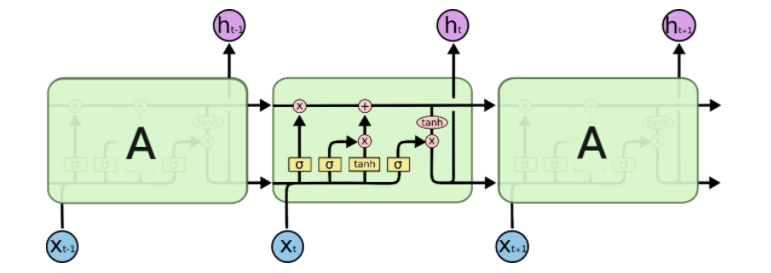
\includegraphics[width=\linewidth]{./assets/background/LSTM.png}
  \caption{Figure taken from \cite{colahLSTM}. The internals of the LSTM cell, and the recurrent flow which is repeated for three consecutive timesteps $t-1, t, t+1$. 
  The LSTM produces an hidden representation at every steep $h_{t-1}, h_{t}, h_{t+1}$ given some inputs $x_{t-1}, x_t, x_{t+1}$.
  }
  \label{fig:lstm_internals}
\end{figure}

Notice that the flow has a direction, and that in this case, the flow moves towards a positive direction of the sequence (i.e. from $t-1 = 0$ to $t + 1 = 2$ for example).

Specifically, LSTMs \cite{hochreiter97} are good at estimating the probability of word $w^{(t)}$ occurring given a previous history of words $w^{(t-1)}, \ldots w^{(1)}$.
In practice, the LSTM is a popular choice for sequence modeling tasks, as it can very well capture the following probability distribution.

\begin{equation}
p\left(w_{1},  w_{2}, \ldots, w_{T} \right)=\prod_{k=1}^{T} p\left(w_{k} | w_{k-1}, \ldots, w_{2}, w_{1}\right)
\end{equation}

\section{GLUE}\label{appendix:GLUE}

\subsubsection{Single Sentence Tasks}

The Corpus of Linguistic Acceptability \textbf{CoLA} \cite{warstadt2018} consists of english sentences, where the task of the model is to predict whether or not the sentence is a valid english sentence.
The Matthews correlation evaluates the model from a score of -1 to 1, where 0 corresponds to uniformly random guessing.
The test set includes out of domain sentences.

\begin{verbatim}
label:1
The professor talked us into a stupor.
\end{verbatim}

\begin{verbatim}
label:0	
The professor talked us.
\end{verbatim}

The Stanford Sentiment Treebank \textbf{SST-2} \cite{socher2013} consists of sentences from movie reviews and human annotations of their sentiment.
This is a binary classification (positive / negative) task.

\begin{verbatim}
label:1
comes from the brave , uninhibited performances
\end{verbatim}

\begin{verbatim}
label:0
excruciatingly unfunny and pitifully unromantic
\end{verbatim}

\subsubsection{Similarity and paraphrase tasks}

The Microsoft Research Paraphrase Corpus \textbf{MRPC} \cite{dolan2005} is a corpus of sentence pairs automatically extracted from online news sources, with human annotations whether the sentences in the pair are semantically equivalent.
Here, an F1-score is taken, because the class-sets are imbalanced.


\begin{verbatim}
quality:1	
Prosecutors filed a motion informing Lee they intend to seek the death penalty.	
He added that prosecutors will seek the death penalty.
\end{verbatim}

\begin{verbatim}
quality:0	
A former teammate , Carlton Dotson , has been charged with the murder.	
His body was found July 25 , and former teammate Carlton Dotson has been charged in his shooting death .
\end{verbatim}

The Quora Question Pairs \textbf{QQP} \cite{shankar17} dataset is a collection of question and answer pairs from the website Quora. 
The task it to check whether a pair of questions are semantically equivalent.
Again, the F1-score is taken as a measure because the class-sets are unbalanced.


\begin{verbatim}
My Galaxy ace is hang?	
Why are the people on Staten Island are racist?	
0
\end{verbatim}

\begin{verbatim}
Where can I learn to invest in stocks?	
How can I learn more about stocks?	
1
\end{verbatim}

The Semantic Textual Similarity Benchmark \textbf{STS-B} \cite{cer2017} is a corpus of pairs of news headlines, video and image captions.
Each pair is annotated with a similarity score from 1 to 5, and the task is to predict these scores.
The evaluation is done using Pearson and Spearman correlation, as the determining factor is the relative ranking amongst scores.


\begin{verbatim}
The man is riding a horse.	
A man is riding on a horse.	
5.000
\end{verbatim}

\begin{verbatim}
A man is playing a guitar.
A girl is playing a guitar.	
2.800
\end{verbatim}


\chapter{Other lines of work}

\section{Clustering}\label{appendix:Clustering}

\paragraph{Affinity Propagation} was first introduced by \cite{frey07}.
Affinity propagation takes as input measures of similarity between pairs of data points. 
Real-values messages for multiple iterations are exchanged between data point until clusters start to emerge.
Initialization happens by assigning the same class to close-enough points, message passing and the choice of which candidate sample to take on happens as defined by a \textit{preference} threshold.

\paragraph{DBScan} is a density based clustering algorithm \cite{ester96} which initiates by finding representative samples that are in regions of high density, and expands clusters from there on.
Due to the density criteria, the resulting clusterings don't have to be convex as is the case with k-means for example. \textbf{HDBScan} is a hierarchical extension of the DBScan algorithm \cite{campello13}. \textbf{Optics} \cite{mihael99} is another extension of DBScan which keeps the cluster hierarchy for a variable neighborhood radius.

\paragraph{MeanShift} is a centroid-based clustering algorithm \cite{comaniciu02}.
After cluster-centers are randomly initialized, the centroids are updated by the mean of the cluster until convergence in the cluster-assignments is reached.
A final post-processing step removes near-duplicate clusters.


\section{Static word embeddings and contextual word embeddings}

The general idea behind distilling static word embeddings from contextual word embeddings is that one can arrive at a (1) compressed representation of the contextual word embedding, and (2) capture polysemous concepts through multiple static word embeddings rather than one embedding per token. 
We present a few ways static word embeddings can be distilled from BERT.

This includes  distilling knowledge or minimizing BERT to smaller neural network models \cite{tang19}, \cite{tsai19}, and most famously \cite{sanh19}.
Compressed sentence representations can also be learned i.e. through random projections or architectures similar to autoencoders \cite{shen19}, amongst others, making use of a max-pool operator over sentence-tokens to arrive at a sentence embedding. \\

\cite{shin18} analyse properties of static word vectors by applying eigenvector analysis from Random Matrix Theory.
The authors show that semantically coherent groups not only form in the row space, but also in the column space, implying that individual word vector dimensions can be interpreted as human-interpretable semantic features.
The authors make use of positive pointwise mutual information matrix, which is based on a log-ratio between the joint probability of a word $w$ and its context words $c$.
The authors apply a qualitative analysis by examining the top elements of the eigenvectors by sorting their absolute values in decreasing order.
The authors analyse salient columns for words like airport.
High absolute values imply that the word is relevant to the semantic group formed in the rowspace.

\cite{whitaker19} follow a similar and more rigorous analysis with static word vectors. 
The authors argue that for standard word vectors, downstream tasks rely much more on local similarity rather than absolute positioning, and thus improving modern language models should focus explicitly on local geometric structures in sampling and evaluation methods.

\section{Metric Learning and Disentanglement}
\label{appendix:metric_learning}

Although difference metric spaces can be considered, we will be referring to Euclidean spaces for simplicity and unless otherwise stated.

Metric learning is the concept of learning a new space in which distances between data samples 

Distance metric learning approaches the problem of learning a similarity metric.

We introduce two sets of data-sample pairs, $S$ and $D$:

\begin{align}
S &= \{ (x_i, x_j) : x_i and x_j should be similar\} \\
D &= \{ (x_i, x_j) : x_i and x_j should be dissimilar\}
\end{align}

As is also mentioned in \cite{moutafis17}, the proximity relation can also be captured through \textit{relation triplets}

\begin{align}
R &= \{ (x_i, x_j, j_l) : x_i is more similar to x_j than x_l \} \\
\end{align}

The general notion of a distance in the euclidean space can be defined as 
\begin{equation}
d_{E}\left(\boldsymbol{x}_{\boldsymbol{i}}, \boldsymbol{x}_{\boldsymbol{j}}\right)=\sqrt{\left(\boldsymbol{x}_{i}-\boldsymbol{x}_{j}\right)^{\top}\left(\boldsymbol{x}_{i}-\boldsymbol{x}_{j}\right)}
\end{equation}
or equivalents as the $l_2$-norm

\begin{equation}
d_{E}\left(\boldsymbol{x}_{i}, \boldsymbol{x}_{j}\right)=\left\|\boldsymbol{x}_{i}-\boldsymbol{x}_{j}\right\|_{2}
\end{equation}

Most distance learning techniques propose different ways of learning a Mahalanobis distance \cite{mahalanobis36}

\begin{equation}
d_{M}\left(\boldsymbol{x}_{i}-\boldsymbol{x}_{j}\right)=\sqrt{\left(\boldsymbol{x}_{i}-\boldsymbol{x}_{j}\right)^{\top} \boldsymbol{A}^{-1}\left(\boldsymbol{x}_{i}-\boldsymbol{x}_{j}\right)}
\end{equation}

Because calculating $d^2$ is computationally simpler, and $d^2$ maintains most mathematical properties as calculating $d$, often $d^2$ is used for downstream calculations (i.e. optimization, distance measure), rather than $d$.

In the case of the Mahalanobis distance, $A$ is a linear operator such as a matrix.
However, $A$ can also be generalized to a nonlinear operator by using the following formulation of the distance metric

\begin{align}
d_{M}^{2}\left(x_{i}-x_{j}\right) &=\left(x_{i}-x_{j}\right)^{\top} A^{-1}\left(x_{i}-x_{j}\right) \\
d_{M}^{2}\left(x_{i}-x_{j}\right) &= (L\left(x_{i}-x_{j}\right))^{\top} (L\left(x_{i}-x_{j}\right)) \\
d_{M}\left(x_{i}-x_{j}\right) &=\left\|L\left(x_{i}-x_{j}\right)\right\|_{2} \\
d_{M}\left(x_{i}-x_{j}\right) &=\left\|Lx_{i}-Lx_{j}\right\|_{2}
\end{align}

where $A = L^T L$ and $L$ can now be any function $L \in \mathbf{R}^n -> \mathbf{R}^d$. 
Whenever, $d < n$, the data is projected to a lower dimensional space $d$, which results in dimensionality reduction, which however breaks the convexity property if $L$ is not invertible.
In comparison to a dimensionality reduction such as PCA, it has been obsereved that learning a similarity measure can sometimes be more effective \cite{chechik10}.

Specifically, the data is projected into another  \
The authors in \cite{moutafis17} argue that due to this property of measuring similarity between pairs, the metric learning models are able to generalize better across classes.

\subsubsection{Non-Deep Metric Learning}

Although we focus on deep metric learning during our experiments, due to the additional flexibility that deep neural networks provide, a good understanding of the underlying mechanisms is useful.

\cite{suarez19} provides a good introduction into the literature of metric learning algorithms.

We first define by a proper definition of a distance

\newtheorem{mydef}{Definition}
\begin{mydef}
Let $X$ be a non empty set. A \textit{distance} or \textit{metric} over $X$ is a map $d: X \times X -> \mathbb{R}$ that satisfies the following properties:

\begin{enumerate}
\item Coincidence: $d(x, y) = 0 \iff x = y,$ for all $x, y \in X$
\item Symmetry: $d(x, y) = d(y, x)$ for all $x, y \in X$
\item Triangle inequality: $d(x, z) \leq d(x, y) + d(y, z) $ for all $x, y \in X$
\end{enumerate}
The ordered pair $(X, d)$ is called a metric space. 
We will be assuming a euclidean metric space unless otherwise specified.
\end{mydef}

Because the coincidence property is not always important to us, but because word-embeddings are more interested in measuring relative distances, we will also consider mappings konwn as \textit{pseudoinstances} which relax the coincidence property to merely fulfill $d(x, x) = 0$.
In the $d$ dimensional euclidean space, the set of \textit{Mahalanobis distances}, which is parametrized by positive semidefinite matrices are useful.

Using above similarity, dissimilarity and relation triplets, an optimal distance $d$ from a set of distances $\mathcal{D}$ can be found

\begin{equation}
\min_{d \in \mathcal{D}} l (d, S, D, R)
\end{equation}

where $l$ is one of the loss metrics shown below.



\begin{figure}[H]
	\center
  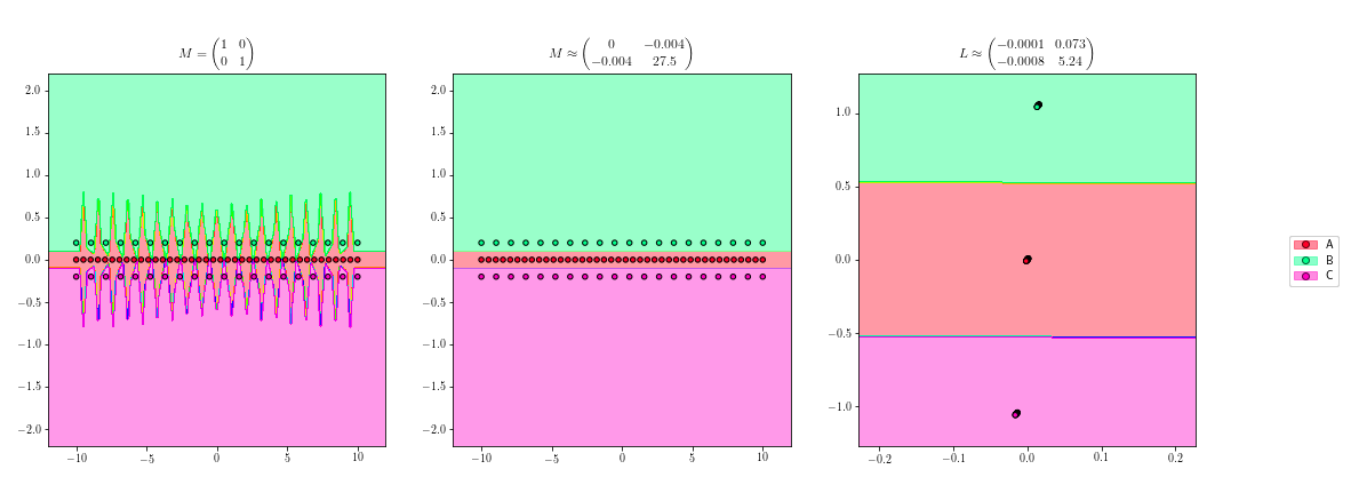
\includegraphics[width=\linewidth]{./assets/relatedwork/metric_learning_example.png}
  \caption{Taken from \cite{suarez19}. The individual tiles show the kNN prediction regions by color for every point in the image. Using the unmodified euclidean distancee, this would result in classification regions on the left. The reader can see, learning an appropriate distance, the classification is much more effective (middle). Finally, the dimensionality is also reducable with this dimension while still matching the classification accuracy (right).}
\end{figure}

Although we will not go into too much detail, we will outline some algorithms that \cite{suarez19} mentions in their work.

We will first start with dimensionality reduction techniques, then move to nearest neighbors classifiers, follow with nearest centroids classifiers and finally go over some information theory based algorithms.
Notice that for almost each one of these methods, kernelized versions are available.


\paragraph{Dimensionality Reduction} techniques include principal component analysis \textit{PCA}, LDA ANMM



\subsubsection{Deep Metric Learning}

Besides the non-deep proposed in the work above models , in\cite{kaya19} also introduces the deep generalization to these frameworks.

\begin{figure}[H]
	\center
  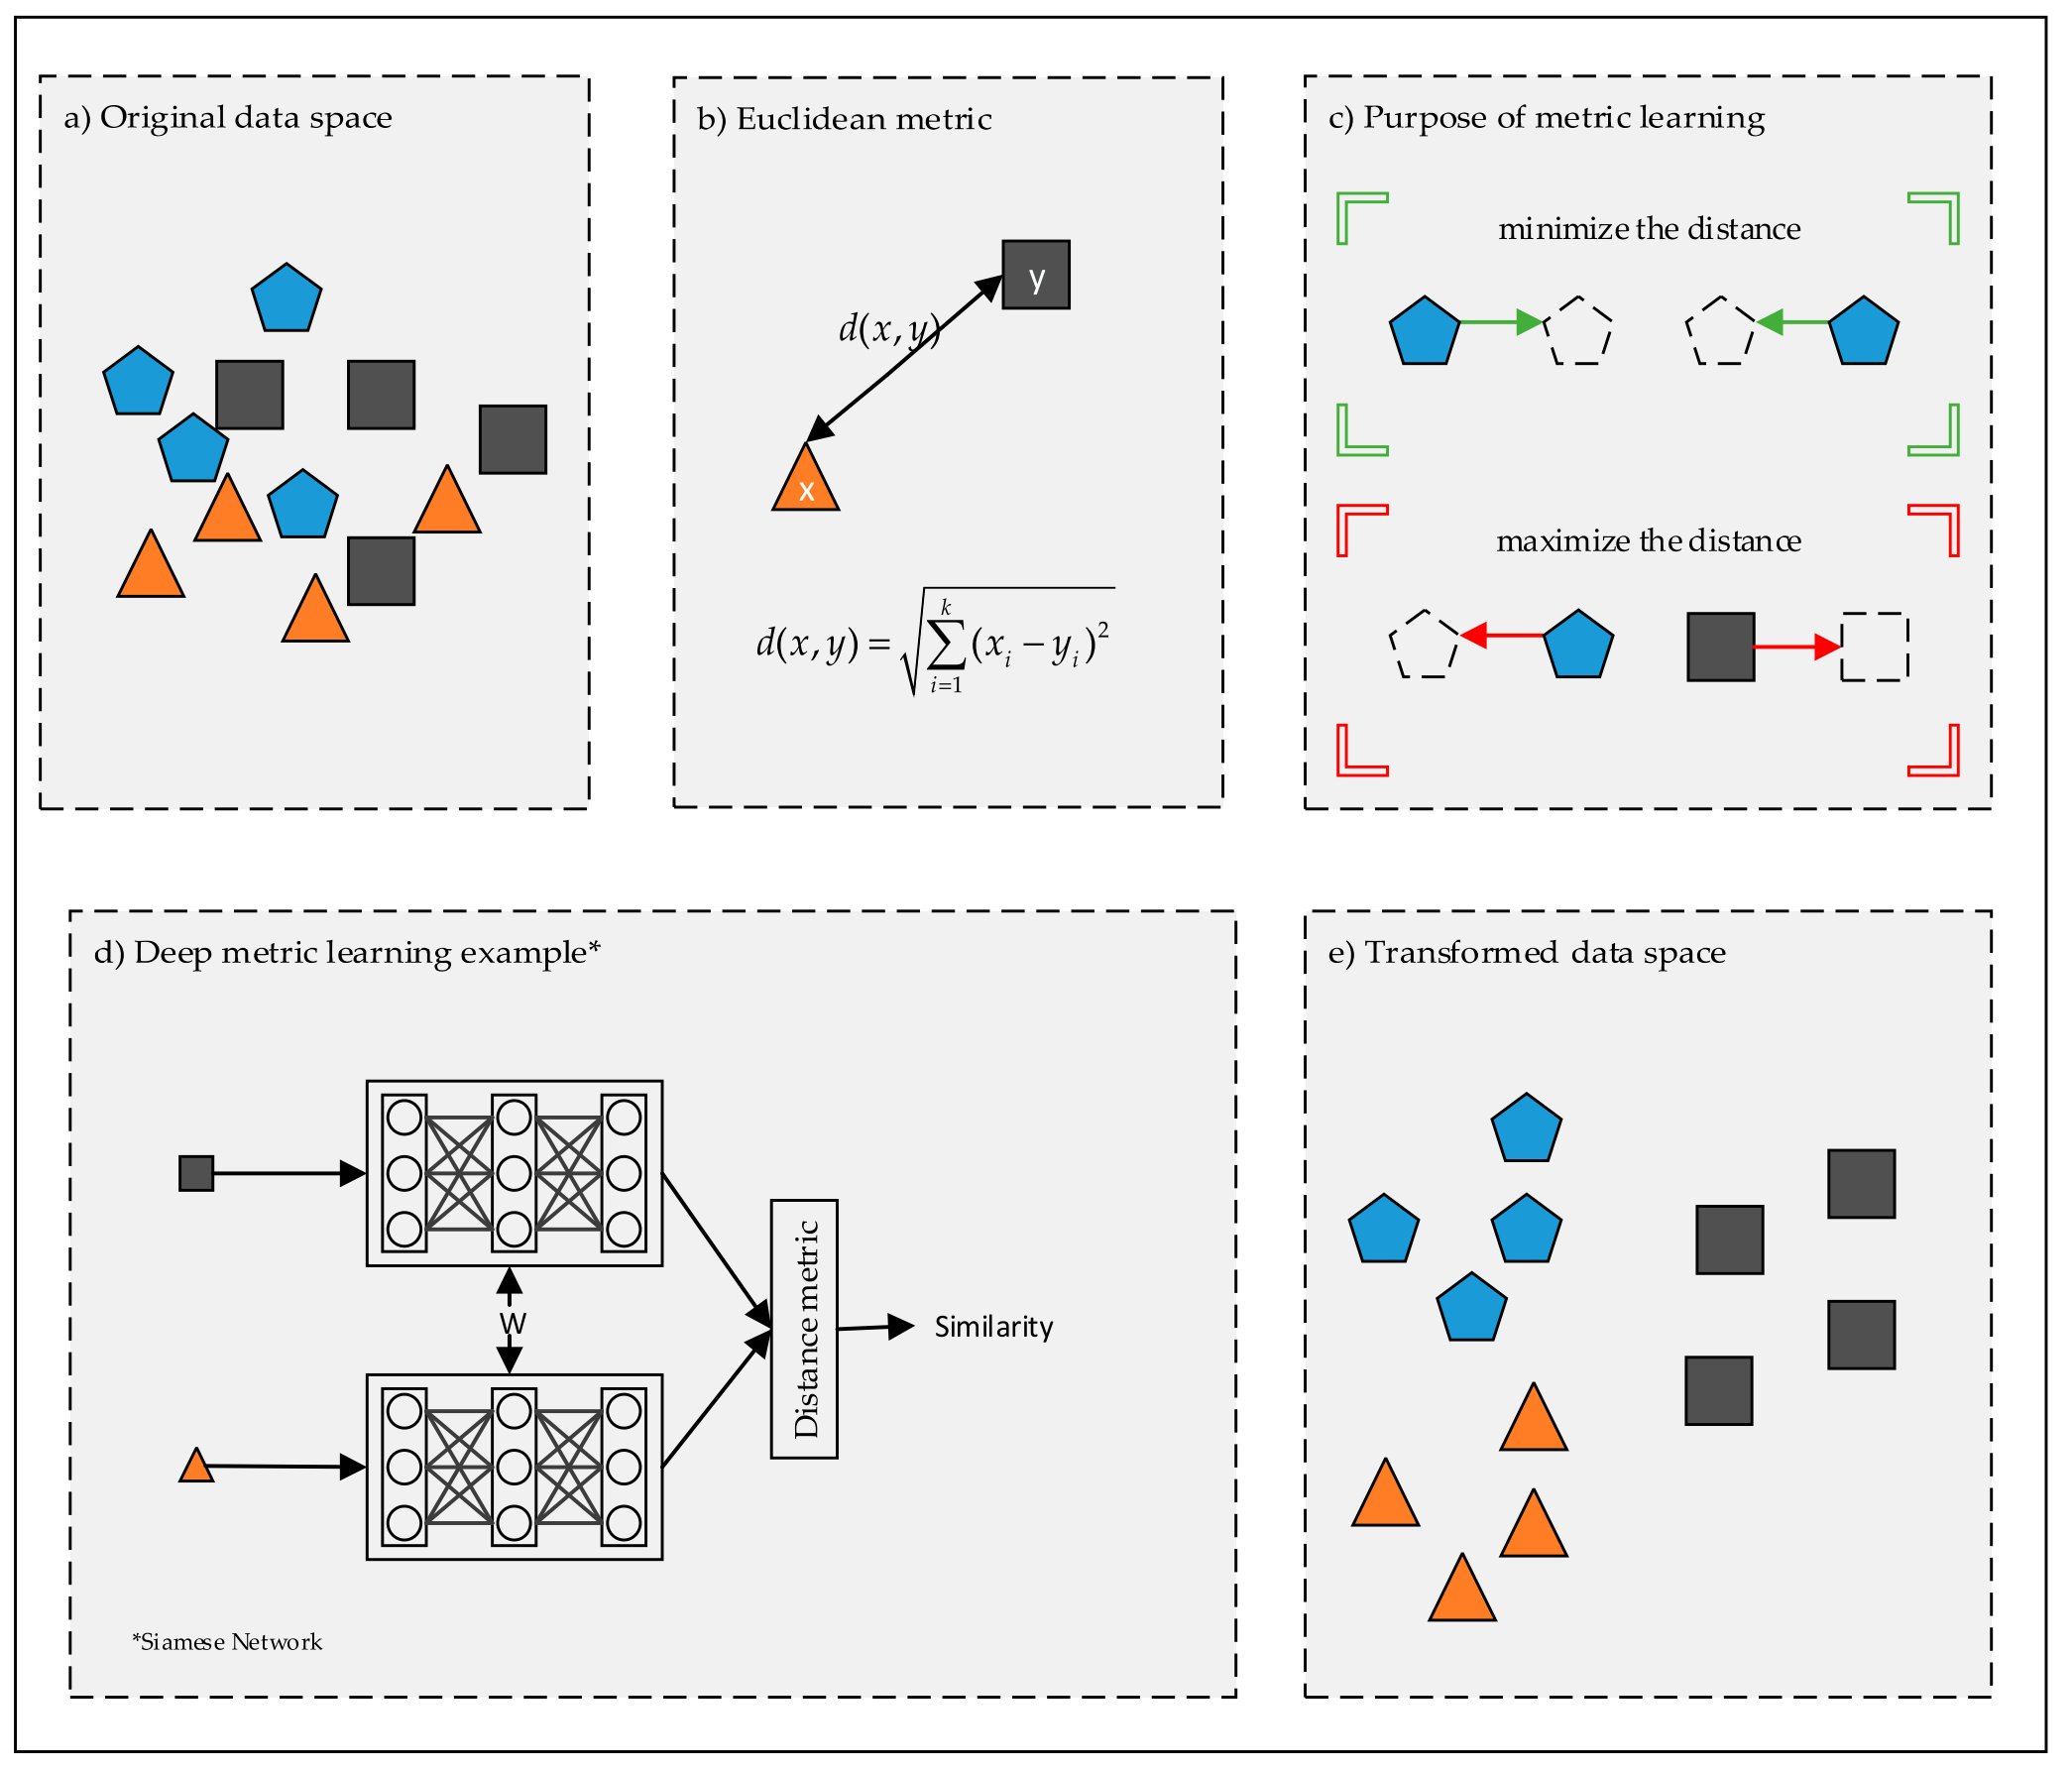
\includegraphics[width=\linewidth]{./assets/relatedwork/metric_learning.png}
  \caption{Taken from \cite{kaya19}. An illustration of deep metric learning. The space is transformed in such a way, that similar object are closer to each other, and dissimilar objects are moved away from each other.}
  \label{fig:muse_translation}
\end{figure}

The most prominent model is the siamese network \cite{bromley94}, \cite{chopra05}, \cite{hadsell06}, where the network consists of two identical sub-networks joined at their outputs. 
We provide an example the architecture looks that looks as follows:

\begin{verbatim}
class Siamese:

    def __init__(input_dim, latent_dim):
        self.fully_connected = nn.Linear(input_dim, latent_dim)
        
    def forward(input1, input2):
        latent_1 = self.fully_connected(input1)
        latent_2 = self.fully_connected(input2)
        
        distance = torch.sqrt(
            torch.sum((latent_1 - latent_2) * (latent_1 - latent_2))
        )
        
        return distance, latent_1, latent_2
\end{verbatim}

Two samples are ingested by the neural network simultaneously.
Both samples are passed through identical weights.
Training occurs by minimizing the contrastive loss.

\begin{equation}
L_{\text {Contrastive }}=(Y) \frac{1}{2}\left(D_{W}\right)^{2}+(1-Y) \frac{1}{2}\left\{\max \left(0, m-D_{W}\right)\right\}^{2}
\end{equation}

where we follow the convention that $Y=1$ whenever the given sample-pairs are of the same class, and $Y=0$ whenever the given sample-pairs are from different classes, and $D_W$ is the output of the above neural network.
Training can be highly unstable, and as such, the learning rate must be properly set, batches must have a balanced amount of both similar, and dissimilar pairs. 
Finally, training can fail if a single batch includes multiple domains of data. \\

For the triplet networks \cite{hoffer14} which makes use of relation triplets, including an input $X$, a point similar to the input $X^p$ and a point dissimilar to the input $X^n$, the following loss can be used for minimization.

\begin{equation}
L_{\text {Triplet}}=\max \left(0,\left\|G_{W}(X)-G_{W}\left(X^{p}\right)\right\|_{2}-\left\|G_{W}(X)-G_{W}\left(X^{n}\right)\right\|_{2}+\alpha\right)
\end{equation} 

where $\alpha$ forms a distance margin, similar to the length of the support vector in SVMs.

As the authors suggest, using a triplet logic results in more stable training and bigger margins between similarity classes.
Analogous logic goes for quadrupel loss etc., but it is unsure to what extend these extensions increase performance.
This general idea can also be extended to angular distance (using cosine distances), and non-euclidean spaces, however, we will not go into further detail on this as this is not the focus of this work.

Although we will not go into further detail, other loss functions include histogram loss \cite{ustinova16}, the structured loss \cite{song16} n-pair loss \cite{sohn16}, magnet loss \cite{rippel16}, angular loss \cite{wang17}, quadruple loss \cite{ni17}, clustering loss \cite{song17}, hierarchical triplet loss \cite{ge18} and the multi-similarity loss \cite{wang19c}.

\subsection{Embeddings for translation}

A lot of work is done in the field of analysing embeddings for translation tasks, to further mitigate the black-box behvaior of neural network.

This includes \cite{kudugunta18} who use singular value canonical correlation analysis to compare hidden representations of language models between different languages.
To arrive at a sentence-representation, they do mean-pooling over the outputted embedding-vectors of a sentence. 
They find interesting behavior in the arrangement of context-embedding in the Transfoerm-Big architecture proposed in the \cite{vaswani17} paper, which is also inherently used in BERT and GPT.
Interestingly, they show that different languages do not project into similar spaces, thus making zero-shot learning tasks between languages difficult.


\begin{figure}[h]
	\center
  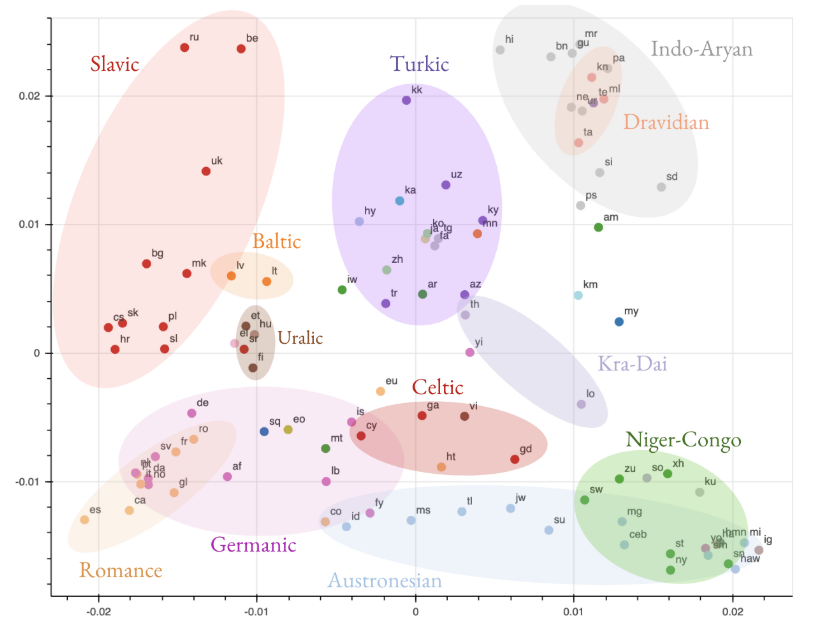
\includegraphics[width=0.6\linewidth]{./assets/relatedwork/embeddings_by_language.png}
  \caption{From \cite{kudugunta18}, visualizing clustering of the encoder representations of all languages, based on ther SVCCA similarity.}
  \label{fig:embeddings_by_language}
\end{figure}


\cite{lample18} uses a cyclic loss to apply unsupervised machine translation suign monolingual corpora only. 
Here, sentence-embeddings are learned over time, which follow the cyclic loss constraint, and minimize the sunsupervised translation loss.

Other work tries to disentangle the different linguisitc, visual and audio-based features by supplying multi-modal input at once \cite{ma19}.
A translation model is learned which can not only translate between different domains, but also between different modalities (i.e. from image to audio, audio to text, and any such combination).


\section{Compressing the non-lexical out}

\subsubsection{Motivation}
\subsubsection{Experiment setup}

We conduct three experiments.

First, we use a simple algorithm to what extent we can disentangle the semantic space within a single sampled word.

The, we use a simple algorithm to what extent we can disentangle the semantic space within multiple sampled words, where we assume that the underlying semantics should again be mutually exclusive (i.e. the sampled words are not independent towards each other.

Finally, we use a simple algorithm to what extent we can disentangle the semantic space within multiple sampled words, where we don't inject any assumptions upon the underlying semantics of the words, i.e. the words are independent towards each other.


\subsubsection{Results}


\chapter{More Results}

\section{Finding the best clustering model}\label{section:more_clustering_results}

\subsubsection{Quantiative Evaluation}

\captionof{table}{The maximum ARI score achieved during hyperparameter optimization for the different models as described by experiment for $k=50$ and $n=500$. }
\begin{table}[htbp]
    \centering
    %\begin{tabularx}{\textwidth}{| X | X |}
    \begin{tabularx}{\textwidth}{b|ss}
    \toprule
      {Clustering Model} & {ARI Score}  \\ \midrule
        Affinity Propagation     & 0.001     \\ \hline
        DBScan                        & 0.000      \\ \hline
        HDBScan                      & \textbf{0.328}     \\ \hline
        MeanShift                    & 0.004      \\ \hline
        Optics                         & 0.000      \\ \hline
    \end{tabularx}
\end{table}

\captionof{table}{The maximum ARI score achieved during hyperparameter optimization for the different models as described by experiment for $k=50$ and $n=1000$. }
\begin{table}[htbp]
    \centering
    \begin{tabularx}{\textwidth}{b | ss}
    \toprule
      {Clustering Model} & {ARI Score}  \\ \midrule
        Affinity Propagation     & 0.000     \\ \hline
        DBScan                        & 0.139      \\ \hline
        HDBScan                      & \textbf{0.271}     \\ \hline
        MeanShift                    & 0.005      \\ \hline
        Optics                         & 0.070      \\ \hline
    \end{tabularx}
\end{table}

\captionof{table}{The maximum ARI score achieved during hyperparameter optimization for the different models as described by experiment for $k=100$ and $n=1000$. }
\begin{table}[htbp]
    \centering
    %\begin{tabularx}{\textwidth}{| X | X |}
    \begin{tabularx}{\textwidth}{b|ss}
    \toprule
      {Clustering Model} & {ARI Score}  \\ \midrule
        Affinity Propagation     & 0.000     \\ \hline
        DBScan                        & \textbf{0.215}      \\ \hline
        HDBScan                      & 0.359     \\ \hline
        MeanShift                    & 0.003      \\ \hline
        Optics                         & 0.000      \\ \hline
    \end{tabularx}
\end{table}


\subsubsection{Qualitative Evaluation}\label{appendix:more_clustering_results_qualitative}


\scalebox{0.7}{
\begin{minipage}{\linewidth}
\begin{align}
\texttt{                                                 } & \texttt{ - -} \nonumber \\
\texttt{heavy withdrawals from the British} & \texttt{ bank Northern Rock reignited concern} \nonumber \\
\texttt{                                                 } & \texttt{ - -} \nonumber \\
\texttt{credit card and other consumer loans, forcing the} & \texttt{ bank to set aside \$3.4 billion} \nonumber \\
\texttt{by a mainland Chinese commercial bank in a U.S.} & \texttt{ bank} \nonumber \\
\texttt{Investors fear the} & \texttt{ bank will be forced to write down} \nonumber \\
\texttt{investors hoped that the} & \texttt{ bank had disclosed the} \nonumber \\
\texttt{                                                 } & \texttt{ - -} \nonumber
\end{align}
\end{minipage}
}
\captionof{figure}{Partition 1 for the word \texttt{bank}. This cluster contains \texttt{bank} in the context of national banks as financial institutions. Notice that the sentiment is usually a negative one.}


\scalebox{0.7}{
\begin{minipage}{\linewidth}
\begin{align}
\texttt{                                              } & \texttt{ - -} \nonumber \\
\texttt{I would expect the} & \texttt{ bank by the trail to the left of the road to have been broken down} \nonumber \\
\texttt{                                              } & \texttt{-  -} \nonumber \\
\texttt{The current slowed and swirled alongside a mud} & \texttt{ bank where cows had trodden to the water} \nonumber \\
\texttt{But the} & \texttt{ bank had positioned itself well} \nonumber \\
\texttt{provide plant scientists and farmers with a} & \texttt{ bank of genes} \nonumber \\
\texttt{Upstairs at the large} & \texttt{ bank of cashiers} \nonumber \\
\texttt{                                              } & \texttt{ - -} \nonumber
\end{align}
\end{minipage}
}
\captionof{figure}{Partition 2 for the word \texttt{bank}. This cluster contains \texttt{bank} as a sequence of objects.}


\scalebox{0.7}{
\begin{minipage}{\linewidth}
\begin{align}
\texttt{                                                 } & \texttt{ - -} \nonumber \\
\texttt{of their family’s naturalization - } & \texttt{ bank deposit by bank deposit} \nonumber \\
\texttt{                                                 } & \texttt{ - -} \nonumber \\
\texttt{12 that the company might suffer a run on the} & \texttt{ bank because of mortgage concerns} \nonumber \\
\texttt{Third, per several} & \texttt{ bank managers of major national banks} \nonumber \\
\texttt{Local party bosses gained broad powers over state} & \texttt{ bank lending, taxes} \nonumber \\
\texttt{government contracts, and a web of} & \texttt{ bank accounts} \nonumber \\
\texttt{Prince Bandar’s Washington} & \texttt{ bank accounts} \nonumber \\
\texttt{                                                 } & \texttt{ - -} \nonumber
\end{align}
\end{minipage}
}
\captionof{figure}{Partition 3 for the word \texttt{bank}. This cluster contains \texttt{bank} as a local, consumer bank (in contrast to institutional, national banks).}


\scalebox{0.7}{
\begin{minipage}{\linewidth}
\begin{align}
\texttt{                                                    } & \texttt{- -} \nonumber \\
 \texttt{to lift some of the mystery surrounding the central} & \texttt{ bank and improve communications with Wall Street} \nonumber \\
\texttt{                                                    } & \texttt{- -} \nonumber \\
\texttt{many economists had predicted that the} & \texttt{ bank would not cut its rate} \nonumber \\
\texttt{expectations that the central} & \texttt{ bank will raise interest} \nonumber \\
\texttt{a hint that the central} & \texttt{ bank plans to hold rates} \nonumber \\
\texttt{China’s central} & \texttt{ bank has stepped up its already huge purchases of dollar-denominated securities} \nonumber \\
\texttt{fertilizer prices in African countries, but that the} & \texttt{ bank itself had often failed to recognize} \nonumber \\
\texttt{                                                    } & \texttt{- -} \nonumber
\end{align}
\end{minipage}
}
\captionof{figure}{Partition 4 for the word \texttt{bank}. This cluster contains \texttt{bank} in the context of national banks as financial institutions. Notice that here, the context is usually about interest rates.}


\scalebox{0.7}{
\begin{minipage}{\linewidth}
\begin{align}
\texttt{                                              } & \texttt{- -} \nonumber \\
\texttt{citing challenges for the investment} & \texttt{ bank and the potential for an above-average credit burden} \nonumber \\
\texttt{                                              } & \texttt{- -} \nonumber \\
\texttt{93 percent drop in profits at its investment} & \texttt{ bank last week} \nonumber \\
\texttt{UBS said it did not expect its investment} & \texttt{ bank to return to profitability} \nonumber \\
\texttt{defrauded by the investment} & \texttt{ bank in 1998 when} \nonumber \\
\texttt{said in an interview that the investment} & \texttt{ bank approached him last month \nonumber} \\
\texttt{said the leaders of Citigroup’s investment} & \texttt{ bank and alternative} \nonumber \\
\texttt{                                            } & \texttt{- -} \nonumber
\end{align}
\end{minipage}
}
\captionof{figure}{Partition 5 for the word \texttt{bank}. This cluster contains \texttt{bank} in the context of investment banks (in contrast to consumer, and institutional banks).}

EXAMPLES FOR KEY CLUSTERING

\scalebox{0.7}{
\begin{minipage}{\linewidth}
\begin{align}
\texttt{                                                 } & \texttt{- -} \nonumber \\
\texttt{Many of the} & \texttt{ key Arab states } \nonumber \\
\texttt{                                                 } & \texttt{- -} \nonumber \\
\texttt{in two months and Australia's} & \texttt{ key S\&P ASX 200 shed 1.9 percent } \nonumber \\
\texttt{Wall Street rebounded Wednesday after} & \texttt{ key earnings reports from JPMorgan Chase \& Co.} \nonumber \\
\texttt{The Democratic candidate hires a} & \texttt{ key strategist} \nonumber \\
\texttt{[CLS] Mr. Jones “quickly established a good rapport with} & \texttt{ key donors” } \nonumber \\
\texttt{able to meet the two} & \texttt{ key officials in the government} \nonumber \\
\texttt{                                                 } & \texttt{- -} \nonumber
\end{align}
\end{minipage}
}
\captionof{figure}{Partition 1 for the word \texttt{key}. This cluster contains \texttt{key} as a synonym for the word \texttt{main}, which characterizes an important subject. The context is one between large institutions in politics and finance. The sentiment is generally positive.}



\scalebox{0.7}{
\begin{minipage}{\linewidth}
\begin{align}
\texttt{                                                 } & \texttt{- -} \nonumber \\
\texttt{former president of Trinity College, who played a} & \texttt{ key role in designing the test} \nonumber \\
\texttt{                                                 } & \texttt{- -} \nonumber \\
\texttt{seen in the West as a} & \texttt{ key yardstick of the fairness of an election} \nonumber \\
\texttt{treat ... as a} & \texttt{ key factor in its decisions about regulatory issues} \nonumber \\
\texttt{which policy makers have called the} & \texttt{ key test for deciding whether to lower interest rates} \nonumber \\
\texttt{9. 11. as a} & \texttt{ key element in pitch meetings} \nonumber \\
\texttt{                                                 } & \texttt{- -} \nonumber
\end{align}
\end{minipage}
}
\captionof{figure}{Partition 2 for the word \texttt{key}. This cluster contains \texttt{key} as a synonym for the word \texttt{main}, which characterizes an important subject. The context is one of regulations and elections. The sentiment is serious.}



\scalebox{0.7}{
\begin{minipage}{\linewidth}
\begin{align}
\texttt{                                                 } & \texttt{- -} \nonumber \\
\texttt{Interstate 5 is a} & \texttt{ key route connecting Southern and Northern California} \nonumber \\
\texttt{                                                 } & \texttt{- -} \nonumber \\
\texttt{ A} & \texttt{ key piece of new functionality for Ops Center } \nonumber \\
\texttt{Youssef Squali at Jefferies \& Co. says two} & \texttt{ key factors are driving the stock up} \nonumber \\
\texttt{transforming connection with believers is a} & \texttt{ key element of evangelical Christianity} \nonumber \\
\texttt{What would you say was the} & \texttt{ key element of your management style that allowed you to stabilize H.P.} \nonumber \\
\texttt{is a} & \texttt{ key indicator of retailer performance} \nonumber \\
\texttt{in the West the} & \texttt{ key players were not a small group of intellectuals reading Greek sources } \nonumber \\
\texttt{                                                 } & \texttt{- -} \nonumber
\end{align}
\end{minipage}
}
\captionof{figure}{Partition 3 for the word \texttt{key}. This cluster contains \texttt{key} as a synonym for the word \texttt{main}, which characterizes an important subject. The context is one of groups of people. The sentiment is neutral to positive.}

\scalebox{0.7}{
\begin{minipage}{\linewidth}
\begin{align}
 \texttt{                                                 } & \texttt{- -} \nonumber \\
\texttt{times change and technology advances, the} & \texttt{ key to the city symbolizes } \nonumber \\
\texttt{                                                 } & \texttt{- -} \nonumber \\
\texttt{And an official, five-and-three-quarters-inch-long gold-plated pewter} & \texttt{ key to prove it} \nonumber \\
\texttt{but it is small enough to fit onto a} & \texttt{ key chain} \nonumber \\
\texttt{In it lay three keys on a} & \texttt{ key chain in the shape of a red speedboat} \nonumber \\
\texttt{                                                 } & \texttt{- -} \nonumber
\end{align}
\end{minipage}
}
\captionof{figure}{Partition 4 for the word \texttt{key}. This cluster contains \texttt{key} as a synonym for the word \texttt{main}, which characterizes an important subject. The context is one of sports and baseball. The sentiment is mixed.}


\scalebox{0.7}{
\begin{minipage}{\linewidth}
\begin{align}
\texttt{                                                 } & \texttt{- -} \nonumber \\
\texttt{The Red Sox will now have all their} & \texttt{ key players from their 2007 championship team} \nonumber \\
\texttt{                                                 } & \texttt{- -} \nonumber \\
\texttt{Mike Green scored 12 points and had a} & \texttt{ key assist in overtime as No. 22 Butler beat Virginia Tech} \nonumber \\
\texttt{or taking the chance of losing a} & \texttt{ key player to injury} \nonumber \\
\texttt{But they never led, could not get a} & \texttt{ key basket at crucial times and played like a team } \nonumber \\
  \texttt{but Cam Long stole the ball near the top of the} & \texttt{ key and ran out the clock} \nonumber \\
\texttt{                                                 } & \texttt{- -} \nonumber
\end{align}
\end{minipage}
}
\captionof{figure}{Partition 5 for the word \texttt{key}. This cluster contains \texttt{key} as a synonym for the word \texttt{main}, which characterizes an important subject. The context is mixed. The sentiment is mixed .}


\scalebox{0.7}{
\begin{minipage}{\linewidth}
\begin{align}
\texttt{                                                 } & \texttt{- -} \nonumber \\
\texttt{Three of their} & \texttt{ key players played more than 40 minutes in Sacramento} \nonumber \\
\texttt{                                                 } & \texttt{- -} \nonumber \\
\texttt{A} & \texttt{ key for the Giants on Sunday} \nonumber \\
\texttt{chemical reactions on solid surfaces, which are} & \texttt{ key to understanding questions like why the ozone layer is thinning} \nonumber \\
\texttt{but is she part of the conspiracy or the} & \texttt{ key to Sim’s salvation?} \nonumber \\
\texttt{whose ability to play on a sprained ankle against the Eagles} & \texttt{ key to that matchup} \nonumber \\
\texttt{Horses have been the lifelong} & \texttt{ key to satisfying the real feminine needs for me and my daughter} \nonumber \\
\texttt{Connecticut cornerback said the} & \texttt{ key to defeating Louisville would be pressuring Brohm} \nonumber \\
\text{                                                 } & \texttt{- -} \nonumber
\end{align}
\end{minipage}
}
\captionof{figure}{Partition 6 for the word \texttt{key}. This cluster contains \texttt{key} as a synonym for the word \texttt{main}, which characterizes an important subject. The context is mixed. The sentiment is mixed.}

\section{Nominalised Verbs}\label{section:frozen_verbs}
The words under investigation include
\Verb#attack#, \Verb#act#, \Verb#die#, \Verb#kick#, \Verb#sand#, \Verb#address#, \Verb#aim#, \Verb#act#, \Verb#address#, \Verb#back#, \Verb#bear#, \Verb#block#, \Verb#catch#, \Verb#charge#, \Verb#crack#, \Verb#double#, \Verb#face#, \Verb#head#, \Verb#march#, \Verb#order#, \Verb#play#, \Verb#roll#, \Verb#saw#, \Verb#tie#, \Verb#train#, \Verb#treat#, \Verb#value#, \Verb#visit#, \Verb#wake#, \Verb#work#, \Verb#zone#, \Verb#act#, \Verb#address#, \Verb#aim#, \Verb#answer#, \Verb#back#, \Verb#balloon#, \Verb#bank#, \Verb#battle#, \Verb#bear#, \Verb#bend#, \Verb#blast#, \Verb#block#, \Verb#break#, \Verb#brush#, \Verb#catch#, \Verb#challenge#, \Verb#charge#, \Verb#cheer#, \Verb#color#, \Verb#cook#, \Verb#crack#, \Verb#curl#, \Verb#cycle#, \Verb#dance#, \Verb#design#, \Verb#die#, \Verb#double#, \Verb#doubt#, \Verb#dust#, \Verb#echo#, \Verb#end#, \Verb#estimate#, \Verb#face#, \Verb#finish#, \Verb#fish#, \Verb#flood#, \Verb#fool#, \Verb#frown#, \Verb#garden#, \Verb#glue#, \Verb#guard#, \Verb#guess#, \Verb#hammer#, \Verb#hand#, \Verb#head#, \Verb#hug#, \Verb#insult#, \Verb#iron#, \Verb#kiss#, \Verb#laugh#, \Verb#loan#, \Verb#love#, \Verb#man#, \Verb#march#, \Verb#milk#, \Verb#object#, \Verb#order#, \Verb#paddle#, \Verb#peel#, \Verb#permit#, \Verb#play#, \Verb#pop#, \Verb#practice#, \Verb#produce#, \Verb#punch#, \Verb#question#, \Verb#quiz#, \Verb#rhyme#, \Verb#rock#, \Verb#roll#, \Verb#run#, \Verb#sand#, \Verb#saw#, \Verb#skate#, \Verb#smell#, \Verb#surprise#, \Verb#thunder#, \Verb#tie#, \Verb#time#, \Verb#toast#, \Verb#trace#, \Verb#train#, \Verb#treat#, \Verb#trick#, \Verb#use#, \Verb#vacuum#, \Verb#value#, \Verb#visit#, \Verb#wake#, \Verb#walk#, \Verb#water#, \Verb#wish#, \Verb#work#, \Verb#x - ray#, \Verb#yawn#, \Verb#zone#, \Verb#cut#, \Verb#break#, \Verb#well#, \Verb#down#, \Verb#run#, \Verb#round#, \Verb#table#, \Verb#bank#, \Verb#cold#, \Verb#good#, \Verb#mouse#, \Verb#was#, \Verb#key#, \Verb#arms#, \Verb#thought#, \Verb#pizza#, \Verb#made#, \Verb#book#, \Verb#damn#.































\chapter{Applications}\label{AppendixApplication}

\section{Using embeddings in other domains}

\cite{tshitoyan19} apply a word2vec type training methodology on chemical publications to encode relationships between chemical compounds.


\section{Using embeddings in translations}


Although word-vectors can be used for a variety of tasks, we will focus on some varieties of how these vectors are used for machine translation (of human languages) tasks.

Amongst the most prominent method is the MUSE model introduced by \cite{conneau17}.
Here, a mapping $W$ is found using either an unsupervised methodology by minimizing the batch-size cosine-distance between sampled word-vectors between two languages $A$ and $B$, or a supervised methodology is devised using the procrustes algorithm.

\begin{figure}[h]
	\center
  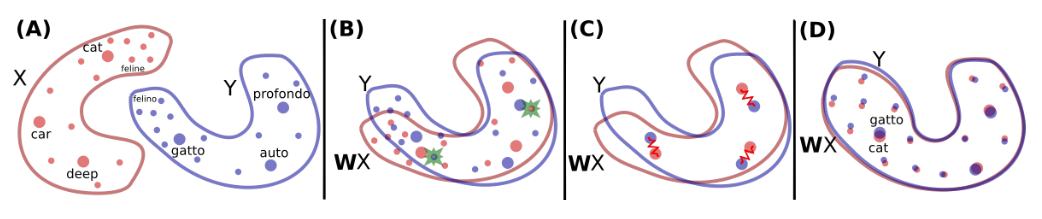
\includegraphics[width=\linewidth]{./assets/relatedwork/muse.png}
  \caption{Taken from \cite{conneau17}. Toy illustration of the embedding matching methodology using the MUSE model.}
  \label{fig:muse_translation}
\end{figure}

Specifically, the following loss-function optimizes over the space of possible mapping matrices $W^*$:

\begin{equation}
W^{\star}=\underset{W \in O_{d}(\mathbb{R})}{\operatorname{argmin}}\|W X-Y\|_{\mathrm{F}}=U V^{T}, \text { with } U \Sigma V^{T}=\operatorname{SVD}\left(Y X^{T}\right)
\end{equation}

Unsupervised training is conducted using a discriminator and a mapping function, where the discriminator's task is to identify the origin-distribution, and the mapping function is supposed to fool the discriminator, resulting in a mapping function which maps all word-emebddings into a common global embedding space.

A generalization of these word vectors to point-vector probability-distributions are captured by \cite{alvarez18}.
Here, the point-vectors are interpreted as point-delta-distributions in the $d+1$ dimensional space.
Common optimal transport methods are coupled with the Gromov-Wasserstein loss to find an orthogonal mapping which maps from vector-space $X$ to vector space $Y$, and thus from the word-token of one language to another.
One way to achieve this is to use the supervised loss-metric and solve the procrustes problem, finding correspondences between the columns of X and columns of Y through:

\begin{equation}
\min _{\mathbf{P} \in O(n)}\|\mathbf{X}-\mathbf{P} \mathbf{Y}\|_{F}^{2}
\end{equation}

with $O(n)=\left\{\mathbf{P} \in \mathbb{R}^{n \times n} | \mathbf{P}^{\top} \mathbf{P}=\mathbf{I}\right\}$.
The resulting algorithm achieves similar performance to MUSE while requiring only a fraction of the computational cost, being able to get competitive results on CPU.

The unsupervised approach deals with finding a transportation map $T$ that fulfills

\begin{equation}
\inf _{T}\left\{\int_{\mathcal{X}} c(\mathbf{x}, T(\mathbf{x})) d \mu(\mathbf{x}) | T_{\#} \mu=\nu\right\}
\end{equation},

where $\mu$ and $\nu$ are the point-delta distributions describing the word-embeddings in the probability space.
The relaxed Kantorovich's formulation is then finally used to reduce this problem to finding a set of transportation plans in a polytopes.

$$
\Pi(\mathbf{p}, \mathbf{q})=\left\{\Gamma \in \mathbb{R}_{+}^{n \times m} | \Gamma \mathbb{1}_{n}=\mathbf{p}, \Gamma^{\top} \mathbf{1}_{n}=\mathbf{q}\right\}
$$

Finally, the cost function

$$
\min _{\Gamma \in \Pi(\mathbf{p}, \mathbf{q})}\langle\Gamma, \mathbf{C}\rangle
$$
is minimized to find an optimal transportation plan.


Another extension is the work by  


\newpage
\subsubsection{Word2Vec}

BERT conditions on the rest of the input sentence.

BERT uses words, subwords and individual characters (in total 30'000) that are then used as tokens.

Idea is to do the following:
Concepts (and thus words), are represented across multiple contexts.
We can create probabilistic word-embeddings by sampling from a corpus the context of a specific word.
From multiple samples of the context-embedding-vector, we take the mean and stddev, or create a GMM if there are multimodal logic (we can check this multimodality by running some sort of rejection sampling algorithm).
Then we have a probability density function (one for each language), and can map one into another.

Perhaps we could split up too high-variance embeddings to multimodal embeddings, depending on their use-cases.

This allows for interpretability in polysemy sentences.

Not using more complex flows implies that the flow itself is not the bottleneck (they probably tried out other flows as well).

Are the individual word-embeddings going to be one big blob with high variance, or is it going to be a multi-modal distribution...?

Another task we may look at is, from a given word-embedding, sample it's context. 
Not entirely sure how to do this with BERT and co.

At what point do we overfit, and at what point do we generalize?


\textbf{Artetxe bilingual token matching through unsupervised machine translation}

- Input is cross-lignual word-embeddings
- Build an unsupervised phrase-based statistical machine translation system
- Derive phrase-based embeddings from input-word-embeddings by taking top 400'000 bigrams and 400'000 trigrams -> take arithmetic mean of word-embedding
- score top 100 close phrases using softmax cosine similarity
- generation of synthetic parallel corpus using this approach
- Then use FastAlign to use parallel corpus to align words
- 

\end{document}
